% Harmonic Information Theory: Foundations
% Foundational Document
% Version 1.0 (2026-03-14)
%
% Compile with: pdflatex main.tex && biber main && pdflatex main.tex && pdflatex main.tex

\documentclass[12pt, a4paper, oneside]{book}

% --- Encoding & language ---
\usepackage[utf8]{inputenc}
\usepackage[T1]{fontenc}
\usepackage[english]{babel}

% --- Typography ---
\usepackage{mathpazo}               % Palatino for text and math
\usepackage[scaled=0.85]{helvet}    % Helvetica for sans-serif
\usepackage{courier}                % Courier for monospace
\usepackage{microtype}              % Microtypographic refinements
\linespread{1.05}                   % Palatino benefits from slightly more leading

% --- Page geometry ---
\usepackage[
  top=3cm,
  bottom=3cm,
  inner=3.5cm,
  outer=2.5cm,
  headheight=15pt
]{geometry}

% --- Math ---
\usepackage{amsmath}
\usepackage{amssymb}

% --- Bibliography ---
\usepackage[
  backend=biber,
  style=apa,
  sortcites=true,
  sorting=nyt,
  uniquename=false
]{biblatex}
\addbibresource{references.bib}

% --- Underscore safety (must load BEFORE hyperref) ---
\usepackage[strings]{underscore}    % _ works in text mode without escaping

% --- Cross-references & hyperlinks ---
\usepackage[
  colorlinks=true,
  linkcolor=darkblue,
  citecolor=darkblue,
  urlcolor=darkblue,
  bookmarks=true,
  bookmarksnumbered=true
]{hyperref}
\usepackage{xcolor}
\definecolor{darkblue}{rgb}{0.0, 0.0, 0.55}

% --- Headers & footers ---
\usepackage{fancyhdr}
\pagestyle{fancy}
\fancyhf{}
\fancyhead[L]{\small\nouppercase{\leftmark}}
\fancyhead[R]{\small\thepage}
\renewcommand{\headrulewidth}{0.4pt}
\fancypagestyle{plain}{%
  \fancyhf{}
  \fancyfoot[C]{\small\thepage}
  \renewcommand{\headrulewidth}{0pt}
}

% --- Chapter & section formatting ---
\usepackage{titlesec}
\titleformat{\chapter}[display]
  {\normalfont\huge\bfseries\centering}
  {\chaptertitlename\ \thechapter}
  {20pt}
  {\Huge}
\titleformat{\section}
  {\normalfont\large\bfseries}
  {\thesection}
  {1em}
  {}
\titleformat{\subsection}
  {\normalfont\large\bfseries}
  {\thesubsection}
  {1em}
  {}

% --- Epigraphs ---
\usepackage{epigraph}
\setlength{\epigraphwidth}{0.7\textwidth}
\renewcommand{\epigraphflush}{center}
\renewcommand{\sourceflush}{center}

% --- Graphics & diagrams ---
\usepackage{tikz}               % Diagrams
\usetikzlibrary{arrows.meta, positioning, shapes.geometric, fit, calc, decorations.pathreplacing}
\usepackage{graphicx}           % External graphics
\graphicspath{{figures/}}       % Image search path
\usepackage{subcaption}         % Subfigures (a), (b)
\usepackage{float}              % [H] placement specifier

% --- Misc ---
\usepackage{booktabs}           % Better tables
\usepackage{tabularx}           % Auto-width columns (X type)
\usepackage{enumitem}           % List customization
\usepackage{csquotes}           % Context-sensitive quotes (for biblatex)

% --- Custom commands ---
\newcommand{\HIT}{\textsc{hit}}
\newcommand{\ratio}[2]{#1\!:\!#2}

% --- Document metadata ---
\title{%
  \textbf{\Huge Harmonic Information Theory}\\[0.6em]
  {\LARGE Foundations}
}
\author{%
  {\normalsize\textsc{Authors}}\\[0.3em]
  {\normalsize Mariano Fern\'andez M\'endez \quad Nicol\'as Ech\'aniz}\\[1.5em]
  {\normalsize\textsc{Compilation and final writing}}\\[0.3em]
  {\normalsize Mariano Fern\'andez M\'endez}\\[1.5em]
  {\normalsize\textsc{Institutional framework}}\\[0.3em]
  {\normalsize Asociaci\'on Civil AlterMundi}\\[1.5em]
  {\normalsize\textsc{Research and development team}}\\[0.3em]
  {\normalsize Anabella Scigliano \quad
  Federico Bonino \quad
  Juli\'an De La Reta}\\
  {\normalsize Mart\'in Fern\'andez M\'endez \quad
  Pablo Bustos \quad
  Saira Asua}\\
  {\normalsize Santiago Cetr\'an \quad
  Sof\'ia Campagnoli}
}
\date{2026}

% ============================================================
\begin{document}

\frontmatter

% --- Title page ---
\maketitle

% --- Legal page ---
% Legal page — Harmonic Information Theory
\clearpage
\thispagestyle{empty}

\begin{footnotesize}
\setlength{\parskip}{0.3em}
\setlength{\parindent}{0pt}

\textbf{\normalsize Harmonic Information Theory}

\textbf{Authors:} Mariano Fern\'andez M\'endez and Nicol\'as Ech\'aniz\\
\textbf{Compilation and final writing:} Mariano Fern\'andez M\'endez\\
\textbf{Institutional framework:} This work was developed and published within the institutional framework of \textbf{Asociaci\'on Civil AlterMundi}.\\
\textbf{Research and development team:} Anabella Scigliano, Federico Bonino, Juli\'an De La Reta, Mart\'in Fern\'andez M\'endez, Pablo Bustos, Saira Asua, Santiago Cetr\'an, Sof\'ia Campagnoli.

\textbf{First digital preliminary edition}\\
\textbf{Place and date of edition:} C\'ordoba, Argentina --- April 2026\\
\textbf{Official source:} [URL OFICIAL]\\
\textbf{Contact:} [MAIL DE CONTACTO]

\copyright\ 2026 Mariano Fern\'andez M\'endez and Nicol\'as Ech\'aniz

Unless expressly indicated otherwise, the original content of this work is distributed under the license \textbf{Creative Commons Attribution 4.0 International (CC BY 4.0)} --- \url{https://creativecommons.org/licenses/by/4.0/}. You are free to copy, redistribute, share, adapt, remix, transform, and build upon this work in any medium or format, including for commercial purposes, provided that you give appropriate credit to the authors, provide a link to the license, indicate if changes were made, and do not suggest that the authors or Asociaci\'on Civil AlterMundi endorse your use or derivative version unless expressly authorized.

\textbf{Suggested attribution:}
Fern\'andez M\'endez, Mariano, and Nicol\'as Ech\'aniz. \emph{Harmonic Information Theory}. 2026. [URL OFICIAL]. Compilation and final writing: Mariano Fern\'andez M\'endez. Institutional framework: Asociaci\'on Civil AlterMundi. License: CC BY 4.0.

\textbf{ISBN:} in process. This version corresponds to an \textbf{official preliminary circulation edition}. Once the corresponding ISBN is assigned, the official PDF bibliographic edition, the website, and the source repository will be updated.

\textbf{Formats and official edition:} The official bibliographic edition of the book is the \textbf{PDF}. The Markdown version and the LaTeX repository are part of the open publication and working ecosystem of the book, but do not constitute by themselves the bibliographic edition with ISBN.

\textbf{Third-party materials:} Images, graphics, photographs, tables, extended quotations, or any other material identified as belonging to third parties are excluded from this license unless expressly indicated otherwise, and retain their respective terms of use.

\textbf{Special permissions, press, and institutional inquiries:} {[MAIL DE CONTACTO]}

\end{footnotesize}


% --- Writing process note ---
% A note on the writing process — Harmonic Information Theory
\clearpage
\thispagestyle{empty}
\vspace*{0.24\textheight}

\begin{center}
\begin{minipage}{0.7\textwidth}
\setlength{\parindent}{0pt}
\setlength{\parskip}{0.95em}
\raggedright

{\Large\bfseries Editorial note on writing and authorship\par}
\vspace{0.4em}
\frontcutdivider[0.09\textwidth]

\vspace{1.2em}

This work was developed by Mariano Fern\'andez M\'endez and Nicol\'as Ech\'aniz, with the assistance of generative artificial intelligence tools ---among them Claude (Anthropic) and Codex/OpenAI--- used as support in tasks of exploration, organization, review, and textual development.

Authorship, conceptual selection, theoretical and editorial decisions, compilation, and final writing belong to the human authors.

\end{minipage}
\end{center}


% --- Table of contents ---
\tableofcontents

% ============================================================
\mainmatter

% --- Introduction ---
% Introduction — Harmonic Information Theory: Foundations

\chapter*{Introduction}
\addcontentsline{toc}{chapter}{Introduction}

Across widely separated domains, patterned relations do more than accompany events; they help stabilize them. Oscillatory systems settle into preferred regimes, coupled processes lock or nearly lock under simple constraints, and signals become more legible when their internal organization is not arbitrary. Ratio, resonance, recurrence, interference, and mode structure keep reappearing where matter, organisms, and interpretive systems must maintain coherence without rigidity. What first looks like a family of local regularities gradually begins to look like a distributed phenomenon: some relations do not merely describe organization after the fact; they participate in making it available.

Physics, neuroscience, psychoacoustics, nonlinear dynamics, ecology, biosemiotics, and computation each encounter that phenomenon under their own vocabularies, scales, and instruments. None of them exhausts it. None can authorize it for all the others. Yet the recurrence becomes difficult to treat as accidental when similar relational patterns keep returning wherever systems must coordinate, discriminate, compress, or remain intelligible under change. The unresolved question is therefore not whether one discipline can annex the rest, but whether an object has been encountered repeatedly without being adequately assembled as an object of inquiry.

The name proposed for that object is Harmonic Information Theory. The proposal does not rest on harmony as ornament, aesthetic residue, or nostalgic metaphysics of proportion. It rests on a narrower and harder claim: some harmonic organizations can function as informational constraints. They make detectable structure more available, reduce descriptive and corrective burden, and produce recurrent functional differences for systems that must register, store, interpret, or respond. In this sense, recurrence is not mere repetition. It is one way in which legibility is stabilized. A field becomes informational here not simply because something happens within it, but because patterned relation changes what can be taken up, retained, and acted upon.

Such a proposal remains serious only if its claims are stratified from the beginning. Some parts of the argument stand on convergences already visible across established literatures. Some move one step further and coordinate those convergences into stronger inferences. Others remain explicitly conjectural, however fertile they may prove for the program that follows. This hierarchy is not a gesture of caution added for appearances. It belongs to the method itself. A field is not founded by declaring its strongest possibilities already demonstrated; it is founded by distinguishing what has been observed, what has been inferred, and what remains open enough that later inquiry could genuinely alter its standing.

The same methodological demand governs the role of instruments. Neural networks, computational models, and acoustic devices appear here neither as ornaments of modernity nor as privileged access points to reality. They are constructed probes. They intervene, register, and expose relations under controlled conditions; they help produce controlled settings within which a claim can become sharper, weaker, or newly testable. Phideus and the Harmonic Beacon belong to the manuscript in exactly this sense. They do not settle the ontology by fiat. They extend the range of inscription through which harmonic organization can be asked explicit questions.

One further figure belongs to the argument, though its full treatment comes later. There are moments when a brief perturbation does not impose order from outside but releases an organization already latent in a medium. The later chapters give that event a name: \emph{Jpsh!} The word is bodily and a little unruly, yet it points to something exact. Certain recognitions arrive neither as deduction nor as revelation, but as constrained release under accumulated pressure. The project gathered itself in that register: not as a finished doctrine seeking examples, but as a pattern that became harder to ignore as convergent evidence kept pressing beyond the vocabularies meant to contain it.

What follows begins with a tendency, enters the problem of dispersion, builds an ontology of relation, turns toward consonance, orders its hypotheses, surveys a convergent state of knowledge, rethinks efficiency and orientation, reaches the activation problem, and only then arrives at the probes through which the proposal submits itself to controlled exposure. The central claim is demanding but bounded: under specifiable conditions, harmonic relations may act as privileged constraints on stability, coupling, interpretability, and informational economy across domains that still lack a common language for them. That is also why Appendix~F can serve as a second entrance to this book. Begin there, let its compression strike once, then return to Chapter~1 and move forward in sequence. Read that way, the appendix can produce an abductive \emph{Jpsh!}: an activation of what lies latent in the structure of the book itself, so that the chapters can be read as the unfolding of a form already struck into legibility.


% --- PART I ---
\part{The Observation and the Problem}
\chapter{The Tendency}

\epigraph{\emph{There is something there that deserves a name.}}{}

This document begins from a deliberately modest observation. Across a set of disciplines that rarely speak to one another in a sustained way, researchers keep returning to a similar family of findings: structured relations among oscillatory, wave-bearing, and resonant processes seem to matter more than a purely arbitrary description of events would predict. Simple ratios, recurrent couplings, phase-locked regimes, interference patterns, and mode structures repeatedly appear as privileged constraints rather than as decorative byproducts. No complete theory yet coordinates these findings, and no single mechanism has been demonstrated everywhere. But a recognizable tendency has emerged across multiple literatures, and that tendency has not yet been named, coordinated, or investigated as a coherent field.

The breadth of that tendency is easiest to see when one begins not with music but with physics. Maxwell's field theory gave one of the decisive modern constructions of physical reality in terms of propagation, coupling, and wave-bearing fields rather than inert corpuscles alone \parencite{maxwell_1865}. De Broglie's wave mechanics and the electron diffraction experiments of Davisson and Germer extended that shift into the domain of matter itself, showing that the language of wavelength, interference, and periodic structure was not restricted to optics or acoustics \parencites{debroglie_1925}{davisson_1927}. More recent physics does not collapse into a single ontology, but it repeatedly preserves the same grammar: gravitational waves become observable events within a scientific construction of spacetime rather than speculative metaphor \parencite{abbott_2016}, and pattern formation in driven media appears across classical and quantum systems alike, from Faraday instabilities to Bose-Einstein condensates \parencites{engels_2007}{nguyen_2019}. Taken together, these developments make intelligible a research program that treats relation, mode structure, and resonance as candidates for explanatory priority.

The tendency is visible with particular clarity in neuroscience. Work on neural resonance has argued that tonal perception is not adequately described as passive registration of isolated frequencies, but rather as the dynamic entrainment of oscillatory systems to structured periodic relations \parencites{large_2012}{large_2005}. Research on cross-frequency coupling likewise suggests that simple phase-amplitude or phase-phase relations can operate as integrative mechanisms in the brain rather than as incidental byproducts of neural activity \parencite{canolty_2010}. More recent work on traveling waves and eigenfrequency structure extends this point: ratios among local frequencies may help coordinate geometric and computational organization across cortex \parencite{jacobs_2025}. These traditions do not converge on a single doctrine, but they repeatedly indicate that patterned relation is computationally and biologically salient.

Psychoacoustics and the study of vocal and musical structure constitute one especially legible branch of this larger tendency. Classical work on roughness and critical-band interaction framed consonance and dissonance in terms of interference patterns and spectral interaction rather than in terms of isolated tones understood atomistically \parencites{plomp_1965}{helmholtz_1863}. Later approaches complicated that picture by showing that auditory preference and tonal organization are also constrained by the statistics of vocal production and by the physiology of hearing \parencites{schwartz_2003}{bowling_2015}{bidelman_2009}. Parallel traditions built formal measures around periodicity, harmonic entropy, and spectral organization in order to explain why some intervallic relations are more stable, more compressible, or more perceptually coherent than others. The specific models differ, but the broader pattern is stable: harmonic relations are repeatedly treated as privileged constraints on perception and organization.

In ecology and biosemiotics, the same pressure reappears under yet another vocabulary. Krause's work on the acoustic niche hypothesis describes ecosystems as organized fields in which organisms partition spectral and temporal resources rather than emitting indiscriminately into noise \parencite{krause_2013}. The result is not simply coexistence, but patterned coexistence: recurrence, spacing, and non-random occupancy become ecologically meaningful. Biosemiotic traditions, meanwhile, have long argued that living systems do not merely exchange matter and energy; they exchange signs, and those signs depend on forms of recurrence and interpretability that can be stabilized across contexts \parencites{hoffmeyer_2008}{barbieri_2008}. What changes from one domain to another is the ontology of the object under study. What persists is the suspicion that patterned relation is not epiphenomenal. It does work.

The tendency is equally visible in nonlinear dynamics. Kuramoto's framework for coupled oscillators showed in paradigmatic form that simple rational relations are not arbitrary curiosities but privileged sites of phase locking and stable coordination \parencites{kuramoto_1984}{pikovsky_2001}. Arnold tongues, devil's staircases, and related synchronization structures make the point even more sharply: simpler ratios often command wider basins of locking and more robust coordination than more complex alternatives \parencite{strogatz_2000}. Similar mode-locking phenomena also appear in biological oscillators, where cardiorespiratory and other coupled rhythms can settle into stable integer relations rather than arbitrary drift \parencite{glass_1988}. Related work on recurrence has shown that what acoustics names as consonance can be formalized more generally as a measurable property of signal organization: simpler harmonic relations tend to generate stronger and more stable recurrence structure in the time domain \parencite{trulla_2018}. Even visualizations such as Lissajous curves make this point accessible in geometric form: ratio simplicity is expressed as topological simplicity and repeatable closure, not merely as aesthetic preference \parencite{gallozzi_2023}. Here again, the vocabulary differs from neuroscience or psychoacoustics, but the structural intuition is strikingly similar.

Comparative and cross-species work extends the question beyond the human case. Surveys of musicality across species, studies of consonance processing in non-human animals, work on pitch perception across species, and classic motivation-structural rules in vocal communication all suggest that sensitivity to intervallic, harmonic, or structurally patterned relations cannot be treated as an exclusively human cultural artifact \parencites{hoeschele_2015}{toro_2017}{walker_2019}{morton_1977}. The evidence is heterogeneous and should not be smoothed into a false consensus. But that heterogeneity is itself informative: once the question survives changes of species, niche, and task, it begins to look less like a local convention and more like a recurring problem in organized signaling.

At the outer edge of this survey, a smaller but increasingly explicit literature pushes the question further toward mind, matter, and consciousness. The Orch OR line developed by Hameroff and Penrose proposes that coherent quantum processes in microtubular structures may participate in conscious episodes, while Stapp's quantum interactive dualism reopens the causal status of conscious agency within quantum description \parencites{hameroff_2014}{stapp_2005}. Conscious realism and analytic idealism radicalize the displacement from another side by treating spacetime and matter as derivative appearances of a deeper field of conscious relation rather than as self-sufficient primitives \parencites{hoffman_2008}{kastrup_2017a}{kastrup_2017b}. HIT enters this frontier from a different side. It begins with cross-domain evidence of relational organization and only later asks how far the ontological consequences may reach. The existence of these peer-reviewed programs matters here because it shows that questions linking wave, field, matter, and consciousness are active sites of inquiry rather than mere cultural residue.

These literatures do not yet agree on a single explanatory center. What matters is that they keep rediscovering, from within their own methods and their own problems, that certain proportional relations and resonant organizations function as privileged sites of coupling, stability, compressibility, or interpretability. One field calls the phenomenon resonance. Another calls it periodicity. Another frames it as mode locking, wave propagation, harmonic entropy, interference structure, or recurrence. The names change because the local problems change. The structural drift does not.

Harmonic Information Theory therefore begins by naming a convergence problem. There appears to be a distributed empirical intuition, recurring across fields, that structured relations among oscillatory and wave-bearing processes carry or constrain information in ways that matter for physical stability, biological coordination, perception, and signal organization. Yet there is no Ariadne thread linking the literatures. Each field largely cites its own canonical authors, defines its own admissible evidence, and treats adjacent traditions as peripheral at best.

HIT is proposed first as an act of coordination. Its opening wager is disciplined: when multiple domains repeatedly discover that structured relations among oscillatory, resonant, and field-like processes matter, it becomes scientifically reasonable to ask whether those discoveries are shadows of a broader problem that has not yet been properly assembled. This wager does not reduce every important pattern in nature to simple ratios, nor flatten reality into a slogan about vibration. The acoustic and musical literatures matter here because they have developed one of the richest vocabularies for describing such relations. If a real pattern of convergence exists, the next problem is no longer merely empirical. It is epistemic.

\chapter{The Problem of Disciplinary Dispersion}

\epigraph{\emph{What converges in the world disperses in the disciplines.}}{}

If the previous chapter identifies a recurring tendency, the present chapter names the obstacle that has prevented that tendency from becoming an explicit field of inquiry. The obstacle is not simply lack of data. It is disciplinary dispersion. The relevant findings are scattered across neuroscience, psychoacoustics, dynamical systems, ecology, biosemiotics, field theory, wave physics, and computational modeling, but the institutions of knowledge production remain organized around local objects, local methods, and local vocabularies. As a result, neighboring discoveries often remain mutually invisible even when they concern formally adjacent patterns of coupling, recurrence, and resonant organization.

The first barrier is lexical. A neuroscientist speaks of cross-frequency coupling, entrainment, or traveling waves. A psychoacoustician speaks of consonance, roughness, periodicity, or harmonicity. A physicist may instead speak of normal modes, field excitations, interference, coherence, or radiation. A complexity researcher speaks of recurrence, synchronization, and attractor structure. An ecologist may speak of niche partitioning, signal occupancy, or soundscape organization. These vocabularies are not merely superficial labels. They carry with them local ontologies, favored instruments, canonical datasets, and implicit criteria of relevance. What one field treats as a central explanatory variable, another may treat as a derivative artifact or ignore altogether. The result is not outright contradiction so much as non-recognition.

The second barrier is methodological localism. Each domain has built its own evidentiary apparatus around different scales and different objects. Neural recording emphasizes coupling statistics and anatomical interpretation. Psychoacoustics privileges controlled perceptual judgments and spectral models. Dynamical systems research focuses on formal stability and recurrence regimes. Wave physics may privilege interferometry, diffraction, spectral decomposition, or detection of propagating disturbances in media and fields. Ecology tracks population-level organization in real environments. These methodological commitments are justified within each field, but they also make cross-domain synthesis difficult. Evidence that is decisive in one literature may not even count as admissible evidence in another. A recurrence plot, an fMRI coupling map, an optical interference pattern, a gravitational-wave trace, and a perceptual consonance curve can all point toward structured relational organization while remaining institutionally non-convertible.

The third barrier is incentive structure. Scientific communities are rewarded for novelty within recognizable disciplinary boundaries, not for patiently assembling bridges across them. Journals, review cultures, citation practices, graduate training, and conference ecologies all reinforce local coherence. The researcher who frames a result in the accepted language of a subfield is legible, citable, and publishable. The researcher who attempts a transdisciplinary synthesis often risks being judged too speculative for one audience and too technical for another. The same formal pattern may be publishable when framed as cross-frequency coupling in neuroscience, legible when framed as recurrence in nonlinear dynamics, and suspect when framed as harmonicity across domains. In that environment, the safest intellectual strategy is partial rediscovery: solve a local problem with local vocabulary, and leave the larger pattern unnamed.

The result is that even disputes internal to one literature rarely propagate cleanly to adjacent ones. Critical debates on consonance have already shown how difficult it is to separate physiological, cultural, and formal explanatory layers without collapsing them into one another \parencite{parncutt_2011}. Cross-cultural work adds a second constraint. Findings such as those reported for the Tsimane do not invalidate the possibility of broad harmonic regularities, but they do block any easy slide from recurrent structure to universal aesthetic law \parencite{mcdermott_2016}. Similar caution is needed when one moves toward the hard sciences: the fact that multiple domains deploy wave and field concepts does not by itself license the claim that one model is structurally isomorphic to reality in any simple or exhaustive sense.

Galison names one part of this situation through trading zones: scientific subcultures can coordinate locally around exchanges, instruments, and partial contact languages without ever sharing a full ontology \parencite{galison_1997}. Star and Griesemer make the point more concrete. Some objects travel across communities precisely because they are plastic enough to be interpreted differently while remaining robust enough to stay recognizable \parencite{star_1989}. Harmonic relations, recurrence structures, constrained oscillatory couplings, and wave-like mode organizations may already function in practice as proto-boundary objects. The problem is that they have not yet been stabilized as such.

Lotman's semiosphere deepens the picture. Boundaries are not only lines of separation; they are also sites of translation, filtering, and productive asymmetry between heterogeneous spaces \parencite{lotman_2005}. If that is right, then disciplinary borders do not merely block circulation. They shape the terms under which circulation becomes possible. The problem for HIT is therefore not only the absence of contact. It is the absence of a sufficiently shared translational space in which adjacent findings can become mutually legible without losing their specificity.

Calvo's critique of structuralist-model isomorphism marks the limit that such a program must respect from the outset. A useful representational structure is not thereby a literal duplication of the world \parencite{calvo_2006}. HIT does not need to say that an acoustic ratio, a cortical eigenmode, and a field excitation are simply the same thing under different names. It needs the more exact claim that these domains may exhibit family resemblances, formal analogies, and partially translatable organizations worth coordinating without being collapsed into a single structural identity.

The epistemic cost of dispersion is high. First, fields repeatedly reinvent one another's partial insights under different names. Second, claims that should be compared remain incomparable because they are embedded in different measurement traditions. Third, overstatement and understatement coexist. One community may localize a phenomenon so tightly that its broader significance disappears from view. Another may generalize too quickly from a narrow context because it lacks contact with adjacent literatures that would impose constraints. The result is a fragmented landscape in which a real convergence can be simultaneously visible in pieces and absent as an articulated object.

HIT should therefore not be introduced as a finished theory that simply waits to be accepted. That would reproduce the very problem it seeks to solve by imposing premature unity on a heterogeneous empirical terrain. At this stage, HIT is better understood as an epistemic category and a research program: it names the possibility that a family of related findings across several domains can be coordinated into a rigorous inquiry about harmonic relations as informational, dynamical, and biological constraints. What it contributes first is not closure, but a shared problem-space.

Lakatos's language of research programmes gives that posture a precise structure. A program acquires shape when a hard core of commitments is named and a protective belt of revisable auxiliary hypotheses is allowed to vary around it \parencite{lakatos_1978}. In the present case, the hard core can be stated minimally: structured harmonic and resonant relations appear repeatedly as privileged constraints in physical, biological, perceptual, and computational organization, and that recurrence is scientifically worth investigating as such. Around that core remains a protective belt that is deliberately open: which mechanisms matter most, in which domains, under which scales, for which forms of information processing, and with what limits.

Kuhn's account of paradigms clarifies the status of the enterprise from another angle. HIT does not yet constitute a paradigm in any strong sense. It is a pre-paradigmatic convergence across several mature fields, and shared objects of inquiry do not automatically create a common research space \parencite{kuhn_1962}. That is why the program must be built neither as an imperial synthesis that seeks to subsume every neighboring language nor as a timid pluralism that refuses integration altogether.

Popper's demarcation problem adds the complementary requirement. If HIT is to become more than a suggestive umbrella, it must remain vulnerable to informative failure rather than insulated by analogy alone \parencite{popper_1959}. The framework therefore has to distinguish observation from mechanism, convergence from proof, analogy from isomorphism, and suggestive correspondence from experimentally supported inference. Part~II begins from that demand for conceptual precision. The next question is no longer whether a distributed convergence exists, but what, exactly, would count as harmonic information.


% --- PART II ---
\part{Ontological Foundations}
\chapter{Ontology of Harmonic Information}

\epigraph{\emph{A single oscillator can oscillate. Two oscillators can enter into relation. From relation comes interference; from interference, pattern; from pattern, the possibility of differential uptake.}}{}


If the previous chapters established why a coordinated field may now be warranted, the present chapter addresses a prior question: what, exactly, is the object that such a field would study? Harmonic Information Theory cannot remain a useful category of coordination unless it specifies, at least provisionally, what it means by \texttt{information}, why harmonic relations might matter ontologically, and under what conditions an interval can be treated as more than a descriptive convenience. The immediate task is therefore conceptual precision: to define the vocabulary without which later claims about consonance, efficiency, or biological significance would remain equivocal.

The central proposal is deliberately minimal. HIT begins from the possibility that information is not exhausted by symbolic encoding, probabilistic distribution, or the properties of isolated substances. Under some conditions, information may also reside in structured relations among oscillatory, resonant, and wave-bearing processes. More specifically, an interval - understood first as a ratio relation between frequencies or modes and only secondarily as a musical interval in the narrow sense - may function as a minimal carrier of organization insofar as it generates recurrent, scale-robust, and differentially interpretable patterns. This is not yet a completed theory. It is an ontological proposal about what kinds of patterns deserve to count as primary in the first place.


\section{Information as pattern, not only as quantity}


Any ontology of harmonic information must begin by resisting a common simplification: the assumption that \texttt{information} already has one settled meaning and that all further uses are metaphorical deviations from it. In fact, the modern concept of information is already stratified. Shannon's theory remains indispensable because it formalized information as reduction of uncertainty over a space of possible messages \parencite{shannon_1948}. That achievement was decisive. It made information measurable, transmissible, and engineerable. But Shannon's abstraction was also intentionally restrictive: it bracketed semantics, embodiment, and function in order to isolate the formal constraints of communication. That move gave us a rigorous measure of informational quantity. It did not, by itself, settle what kinds of patterns deserve ontological priority in natural systems.

Once one leaves the engineering frame, a second layer becomes unavoidable. Information is not only what reduces uncertainty in a channel; it is also what exhibits structure rather than arbitrariness. In algorithmic and compressibility-oriented perspectives, a pattern is informative not because it is maximally random, but because it admits a shorter and more lawful description than an unstructured aggregate would. Put differently, structure matters because it can be compactly represented, predicted, or regenerated. This does not negate Shannon; it supplements it. The point is that not all informative patterns are equally primitive. Some carry lawlike regularities that allow systems to coordinate with lower descriptive or predictive cost. Dubnov's work on information and musical expectation points in that direction by tying salience to structured predictability rather than to raw uncertainty alone \parencite{dubnov_2004}.

Bateson adds a third layer that is essential for HIT. His well-known formulation of information as "a difference which makes a difference" relocates the question from mere formal distribution to operative consequence \parencite{bateson_1972}. In this register, a pattern counts as informational only if it can alter the state, expectation, or behavior of some receiving system. The advantage of this formulation is that it prevents a purely reified ontology of form. A pattern is not informative simply because an observer can describe it elegantly. It is informative when it is capable of differential uptake, constraint, or effect. This point will matter later when HIT moves from formal interval structure to biological and computational interpretation. At the ontological level, however, the lesson is already clear: information is relational not only because it consists of differences, but because it exists through the possibility of system-level response.

The fourth layer is oscillatory and dynamical. In many natural systems, information does not travel only through symbolic tokens or static states; it is enacted through coupling, recurrence, synchronization, phase structure, propagation, and mode organization. Kuramoto's framework made one part of this intuition formally compelling by showing that some relations among oscillators are dynamically privileged: simple ratios can stabilize coordination regimes that would not emerge under arbitrary mismatch \parencite{kuramoto_1984,strogatz_2000}. In neuroscience, cross-frequency coupling extends this point into living systems: oscillatory relations are not incidental decorations on top of information processing, but often part of the very mechanism by which integration occurs across scales \parencite{canolty_2010}. In physics, the modern vocabulary of fields, waves, and excitations preserves the same structural lesson in a different idiom: what matters is often not the isolated bearer but the patterned organization of modes, their couplings, and their interference.

This does not license the crude slogan that everything is simply "wave" in one undifferentiated sense. Different theories retain different ontological commitments, and no single model should be inflated into the whole of what its own discourse constructs as reality. But it does make one claim newly reasonable: across a wide range of domains, some of the most powerful descriptions of organization are descriptions of patterned relation in time and space. Information, in this register, is associated not only with uncertainty reduction or compressibility, but with the emergence of stable, recurrent, and interpretable organizations among coupled processes.

These four layers should not be collapsed into one another. Shannon is not Bateson; compressibility is not biological meaning; dynamic stability is not yet semantic consequence. But they do converge on a common intuition: information is not exhausted by isolated substances or by raw magnitudes taken one at a time. It is tied to patterned difference, lawful relation, and the possibility of repeatable uptake. For the purposes of HIT, this convergence is enough to justify a working definition. We will treat information, in the broad ontological sense relevant to this project, as a structured relation or detectable pattern in a signal or system that, for a given observer, system, or model, can reduce uncertainty, increase compressibility, and produce a functional difference through recurrent interpretability. Under suitable physical conditions, such patterned relation may also participate in local reductions of effective entropy, but that consequence should not be confused with uncertainty reduction in the narrower Shannon sense. What becomes legible as information is therefore not a transparent window onto the Real, but a structured trace through which the Real imposes itself as limit, resistance, or failure of closure within a model. Harmonic information is then a restricted case of this broader category: information carried, constrained, or stabilized by harmonic relations among oscillatory or mode-bearing processes.


\section{Why relation can be ontologically primary}


This definition becomes intelligible only if relation is allowed genuine ontological weight. Much of modern scientific common sense still leans, often implicitly, on a substance-first picture: things are primary, and relations are later properties among already constituted units. HIT requires a different emphasis. The claim is not that substances dissolve into pure relation, but that some of the most durable regularities in the domains under discussion appear first as patterned coupling, interference, and co-constraint. In such cases, relation is not decorative. It is part of what makes the phenomenon legible at all.\footnote{For a recent engineering instance where information appears as physically realized geometry rather than as a detachable abstract layer, see Jelin{\v{c}}i{\v{c}} et al.\ (2025). Their probabilistic hardware formalism treats the accessibility of states as a consequence of energy-landscape geometry and relative transition structure, not as a property of isolated states considered one by one.}

Heidegger's account of being-in-the-world begins to unsettle the inherited picture at exactly this point. Entities do not first present themselves as inert objects and only afterward acquire significance through external linkage. They emerge within a prior field of worldhood, practice, discourse, and being-with, where relevance and articulation are already in play \parencite{heidegger_1927}. Bohm approaches a related displacement from another direction when he argues that what appears as separation may be the unfolding of a deeper implicate order rather than the final truth of the situation \parencite{bohm_1980}. Simondon and Barad push the point into explicitly relational vocabularies. Individuation, transduction, and intra-action all name processes in which units do not simply precede their relations, but take shape through them \parencite{simondon_1958,barad_2007}. Taken together, these traditions do not erase the world of things. They make it harder to assume that things are self-sufficient first terms and that relation arrives only afterward as a secondary predicate.

Contemporary consciousness-first ontologies push this displacement further. Hoffman's conscious realism treats spacetime as an interface generated by conscious agents, while Kastrup's analytic idealism treats matter as the extrinsic appearance of mentation within a wider field of consciousness \parencite{hoffman_2008,kastrup_2017a,kastrup_2017b}. Whether one accepts these inversions or not, they matter here for a narrower reason. They show that the priority of relation, appearance, and experiential articulation over self-sufficient substance is not confined to continental philosophy or systems biology. It has become an active site of formal and ontological experimentation.

Maturana and Varela provide a biological formulation of the same displacement. In the autopoietic account, a living system is not defined first by the inventory of its material parts, but by the organization of relations through which those parts are continuously produced and maintained \parencite{maturana_varela_1980,varela_maturana_uribe_1974}. This is why their distinction between organization and structure matters so much here. Organization names the invariant relational pattern that defines the system as the kind of unity it is; structure names the concrete material realization through which that organization is instantiated at a given moment \parencite{maturana_1970,varela_1979}. Read cautiously, HIT can borrow a narrow analogy from this distinction. A ratio may function like an organizational invariant, while the particular frequencies, amplitudes, and phases that realize it belong to the order of structure. The point is not that harmonic ratios are living systems. It is that Maturana and Varela supply one of the clearest biological precedents for treating relational pattern as prior to the isolated identity of components.

Operational closure sharpens the same lesson. An autopoietic system is materially open yet organizationally closed in the sense that its operations recursively generate the very network that makes those operations possible. This circularity is not self-identity in the static sense, but productive recurrence. HIT can draw a carefully limited comparison from that form of closure to the way some interference patterns or standing-wave organizations preserve a recognizable relational form under changing energetic conditions. The comparison must remain explicitly limited. A standing wave does not regenerate its own material components and is therefore not autopoietic in the strict sense. What it does share with autopoietic description is a focus on relational invariance under structural variation. That is enough to make Maturana and Varela newly relevant to the ontological wager of this chapter without collapsing biological autonomy into harmonic pattern.

The same problem also becomes visible from outside biological theory proper, which matters here because it shows that recursive organization is not a local intuition of one school alone.

An instructive convergence appears here from a different tradition altogether. In \emph{La tecnica digitalizada}, Fern\'andez M\'endez describes a "relational closure" through which a system of know-how achieves enough internal consistency to sustain itself without the continuous intervention of a subject \parencite{fernandez_2021b}. In the manuscript on digital language, he arrives at a closely related problem from yet another route, connecting recursive formal systems, Godelian incompleteness, and operational closure as conditions under which a system can function without ever becoming complete in the strong sense \parencite{fernandez_sf_digital}. HIT does not need to collapse these trajectories into one doctrine. It only needs to register a structurally significant fact: biology, psychoanalytic theories of work and technique, and the epistemology of computation all converge on the intuition that organization is achieved through recursive relation before it is secured by isolated substantial units.

That shift matters for HIT because the framework is interested in phenomena whose explanatory core often lies in organization among terms rather than in the isolated identity of those terms. A ratio does not become significant merely because two frequencies can be listed side by side; it becomes significant when their relation constrains pattern, recurrence, interference, and uptake. This is why the issue is ontological before it is methodological. If relation were only derivative, harmonic information would always risk appearing as a useful descriptive fiction layered over more fundamental realities. If relation can sometimes belong to the order of what first organizes appearance, then harmonic structure becomes a plausible candidate for primitive description rather than an ornamental afterthought.

From the side of signification, a parallel displacement appears in another idiom. Derrida's account of différance interrupts the fantasy of self-present meaning by insisting that what matters in signification is never fully gathered into a term's supposed identity. In the essay by that name, différance is described as what "is never offered to the present" \parencite{derrida_1982}. Sense therefore depends on spacing, deferral, trace, and differential articulation rather than on pure presence or origin. Read in this register, relation is not an accident that later befalls meaning. It belongs to the conditions under which meaning becomes possible. The sign bears the mark of what it is not; it receives force from intervals, delays, and contrasts that prevent it from coinciding transparently with itself.

Lacan radicalizes the point in a way that is especially pertinent here. His formula that a signifier represents a subject for another signifier refuses the idea that the subject could be located intact at either end of an already completed exchange \parencite{lacan_1966}. The subject is not reducible to \texttt{S1} or \texttt{S2}; it appears as a barred effect of the chain, and of the chain's insertion in the field of the Other. Communication, on this view, is not simply the transport of content between fully present interiors. It is a differential process in which position, address, and intelligibility emerge through articulation. That does not convert HIT into psychoanalysis, nor should it. It does, however, sharpen one of the chapter's central points: informational significance need not be thought as a property lying dormant inside isolated units. It may arise at the level of relation, interval, and sequence.

Jung names a comparable organizing tension within psychology, though in a different vocabulary. The Self, in the analytic tradition, is neither identical with the ego nor simply another content hidden somewhere in the psyche. It names an integrating principle that becomes legible through the dynamic relation between conscious and unconscious life rather than through the sovereignty of either pole taken alone \parencite{jung_1959}. Von Franz makes the point more operational when she describes the Self as an orienting factor irreducible to the conscious personality and visible only through processes of individuation rather than through static introspection \parencite{vonfranz_1964}. Read cautiously, this does not import clinical doctrine into ontology. It shows that even in depth psychology, what organizes the field may be neither a fixed substance nor a self-transparent subject, but a process of relation, tension, and gradual integration.

Lotman's semiosphere gives this relationality a broader semiotic topology. No isolated language or code stands first and only later enters relation; the semiosphere functionally precedes its local formations, and meaning takes shape through boundaries, translations, filters, and asymmetric passages between heterogeneous spaces \parencite{lotman_2005}. Peirce and Bateson deepen the same orientation from adjacent directions. If the sign is irreducibly triadic, and if information appears where a difference makes a difference, then relation cannot be treated as residue. It belongs to the conditions under which distinction, transmission, and effect become thinkable at all \parencite{peirce_1931,bateson_1972}. This does not imply that every relation is informative or that every pattern is semiotic. It implies something more precise: some structured relations may be prior to the units later abstracted from them, and the explanatory burden must sometimes begin there.

Nietzsche's "On Truth and Lies in a Nonmoral Sense" introduces a necessary counterpressure into the entire discussion. Concepts appear there as worn metaphors, and truths as stabilized conventions that have forgotten their figurative genesis rather than as transparent mirrors of self-identical essences \parencite{nietzsche_1873}. The warning does not collapse ontology into arbitrariness. It blocks the temptation to mistake classificatory names for the last word on what there is. Wheeler reopens the same question from another side when he proposes that information may not be mere bookkeeping applied to an already complete world, but part of what makes such a world intelligible in the first place \parencite{wheeler_1990}. Read together, Nietzsche and Wheeler mark a narrow passage: one can take information seriously without reifying every formal structure into metaphysical finality.

The ontological wager of this chapter can therefore be stated more carefully. If relation can be primary in existential, semiotic, and relational-physical vocabularies, then it is not conceptually illicit to ask whether harmonic relations among oscillatory or mode-bearing processes might count as primitive informational structures. The task is neither to reduce the world to one acoustic image nor to inflate formal analogy into exhaustive identity. It is to test whether interval, ratio, recurrence, and patterned coupling belong often enough to the order of first intelligibility that a theory of harmonic information becomes worth building. At that point the burden of proof is no longer conceptual permission. It is empirical reach and theoretical precision.


\section{The interval as a minimal informational carrier}


Within that relational ontology, the interval becomes the candidate unit of interest. An interval, in the sense relevant to HIT, is not primarily a named musical object such as a fifth or a third. It is a ratio relation between oscillatory frequencies or, more generally, between modes capable of entering patterned coupling. In acoustics that relation becomes audible as interval. In other domains it may appear as a ratio between frequencies, periodicities, eigenmodes, or recurrent scales of organization. Given two frequencies, \texttt{f1} and \texttt{f2}, the interval may be written as \texttt{r = f1:f2}. What matters about this relation is not only that two magnitudes stand in comparison, but that their coupling generates an interference pattern with distinctive structural properties.

The first of those properties is scale robustness. If both frequencies are multiplied by the same constant \texttt{k}, the absolute frequencies change but the ratio does not. More carefully stated, the interval's relational organization is preserved up to temporal rescaling. This does not mean that every physical system will respond identically across all scales. Media, thresholds, and receptor dynamics still matter. It means something weaker and crucial: the interval is not defined by absolute pitch, but by proportional relation. That alone makes it a stronger candidate for cross-domain description than any frequency taken in isolation.

The second property is pattern generation. Intervals are not abstract ratios floating above the material world; they generate concrete interference organizations. In visual form, Lissajous figures make this especially intuitive. When perpendicular oscillations stand in simple relations, the resulting curves exhibit repeatable closure, symmetry, and topological economy; when the relations become more complex, the curves become correspondingly less simple and less recurrent \parencite{lissajous_1857,gallozzi_2023}. In driven media, related phenomena appear in standing-wave and Faraday-like pattern formation, where periodic forcing organizes matter into stable spatial regimes \parencite{engels_2007,nguyen_2019}. The visual case does not prove the ontological thesis, but it reveals something important: relation can become visible as form. Cymatic traditions, though often rhetorically overstated, are useful at minimum as reminders that oscillatory relations can leave stable traces in matter and geometry \parencite{jenny_1967}.

The third property is dynamical privilege. In models of coupled oscillation, some ratios are more likely than others to anchor stable mode-locking or recurrence structure, especially once one looks at Arnold tongues, locking regimes, and the broader synchronization literature rather than at isolated equations alone \parencite{kuramoto_1984,strogatz_2000}. Reviews such as Acebron and colleagues help situate this broader terrain of synchronization and partial locking without themselves carrying the entire argument about ratio privilege \parencite{acebron_2005}. In neural and cortical systems, ratios likewise appear not merely as incidental numerical coincidences but as organizing constraints within coupling architectures \parencite{canolty_2010,jacobs_2025}. This does not license the naive claim that "simple ratios are always better." It does support a more exact claim: certain intervallic relations are repeatedly recruited by systems because they afford recurrent and stable coordination. That is exactly the sort of condition under which an informational role becomes plausible.

The fourth property is differential interpretability. An interval functions as an informational carrier only if a system can distinguish it from alternative relations in a stable way. This point returns us to Bateson. A ratio is not informative simply because it can be written. It becomes informative when it constrains behavior, coupling, prediction, or response differently than another ratio would. In this sense, the interval is a candidate minimal carrier because it is the smallest relational unit capable of generating a non-trivial difference in oscillatory organization. A single oscillator can oscillate. Two oscillators can enter into relation. From relation comes interference; from interference, pattern; from pattern, the possibility of differential uptake.

At this point, the central proposal can be formulated more precisely. HIT treats the interval as a minimal informational carrier not because it is musically familiar, but because it satisfies four conditions at once: it is relational rather than substantial, robust under common scaling, generative of recurrent structure, and in principle capable of differential interpretation by receiving systems. None of these conditions alone is sufficient. Together they make the interval the strongest initial candidate for the ontological primitive that this program requires.


\section{A minimal ontological proposition for HIT}


The argument of this chapter can now be compressed into a minimal proposition. Information, in the sense relevant to HIT, should be understood as structured relation with the capacity to generate repeatable difference for a system. Harmonic information is the subset of such information that arises through patterned relations among oscillatory, wave-bearing, or mode-organized processes. An interval is the minimal candidate carrier of that information because it specifies a ratio relation whose organization is preserved beyond any single absolute instantiation and whose interference pattern can, under suitable conditions, be stabilized, distinguished, and acted upon.

This formulation remains deliberately narrower than the broader ambitions often attached to harmonic discourse. It does not yet imply that consonance is universally valued, that harmonic simplicity is always biologically optimal, or that every domain we organize as reality is governed by the same ratio laws. Those are later questions. The present chapter has only secured the weaker but necessary claim that a relational ontology of information is coherent, that oscillatory relations offer a plausible site for such an ontology, and that the interval can be treated as the minimal conceptual unit around which the rest of the framework may be organized.

It is useful, finally, to separate three levels of commitment. The observation is that multiple literatures repeatedly assign explanatory weight to structured harmonic relations. The hypothesis is that intervals can function as minimal informational carriers across heterogeneous systems. The inference, more cautious than a doctrine but stronger than a metaphor, is that HIT should be built on a relational ontology rather than on a substance-first model of information. Everything that follows depends on preserving that distinction.

If this is correct, then consonance cannot be defined as the intrinsic property of a ratio taken in abstraction from medium, timbre, body, and context. Once information is treated as relational, consonance must be treated relationally as well. That is the task of the next chapter.

\chapter{Consonance as a Relational Function}

\epigraph{\emph{Consonance does not belong to the isolated ratio alone.}}{}


If the previous chapter argued that harmonic information is best understood in relational terms, then consonance can no longer be treated as a self-sufficient essence lodged inside a ratio taken in abstraction from every medium, body, and context. The ratio remains indispensable. It would be pointless to deny that simple proportional relations recur across acoustics, dynamical systems, and wave-bearing systems of many kinds with unusual explanatory force. Yet that force is not adequately described by saying that consonance simply inheres in numerical simplicity itself. A ratio does not sound, radiate, interfere, stabilize, or become salient in a vacuum. It does so only within a concrete field composed of modal constitution, physical transmission, coupling regime, receptive organization, and contextual framing. For that reason, the present chapter proposes a stricter formulation: consonance should be understood as a relational function rather than as an intrinsic property of the interval considered in isolation.

This shift is not a denial of structure but a correction of emphasis. HIT does not dissolve consonance into pure relativism, nor does it reduce it to arbitrary taste. It instead claims that the ratio names a privileged relational constraint whose consequences depend on the system in which it appears. One may summarize the point provisionally as \emph{Consonance = F(ratio, modal or spectral constitution, medium, coupling regime, receiver, context).} In the acoustic case, that modal constitution appears as timbre and overtone profile; elsewhere, it may appear as mode structure, propagation condition, or resonant topology. Such a formula should not be read as a finished equation, but as a disciplinary warning. It reminds us that no account of consonance is conceptually complete if it abstracts away from the constitution of the interacting modes, the resonant properties of the medium, the dynamics of the receiving system, and the practical or perceptual horizon in which the relation is encountered.

The term \emph{consonance} is retained here because the acoustic and musical traditions gave this family of problems one of its richest and most durable vocabularies. But the concept, as HIT develops it, should be read more broadly. It names a kind of resonant fit, mode compatibility, or low-conflict coordination that becomes especially legible in the sonic domain without being exhausted by it. The task of this chapter is therefore double: to preserve what the sound-focused traditions discovered, and to prevent those discoveries from being mistaken for the limits of the field itself.


\section{Against the isolated essence of the ratio}


The strongest traditional intuition about consonance is easy to state: simple ratios tend to generate more stable, more coherent, or more easily integrated organizations than complex ones. In acoustics this often appears first as a matter of sounding intervals, but the intuition is not reducible to the auditory case alone. It is grounded in a long history of observation about periodic coincidence, spectral overlap, recurrence, and perceptual organization. From classical acoustics through later psychoacoustics, relations such as $2{:}1$, $3{:}2$, and $4{:}3$ have repeatedly appeared as privileged structures rather than as arbitrary mathematical curiosities \parencite{helmholtz_1863,plomp_1965}. Even when the explanatory models differ, the recurrence of these ratios is too persistent to be dismissed. The problem lies elsewhere. The problem begins when one mistakes this recurrent privilege for a complete ontology of consonance.

The insufficiency of that move becomes clear as soon as constitution enters the picture. Sethares showed with unusual clarity, in the sonic case, that consonance is not fixed by interval alone, but by the relation between intervallic structure and the spectral organization of the sounding bodies involved \parencite{sethares_2005}. The same numerical ratio can behave differently under different timbral conditions because what matters is not merely proportional abstraction, but the alignment or conflict of partials, beating structure, and spectral fit. The broader lesson extends beyond acoustics: a relation acquires its effective character only through the modes that realize it and the medium in which those modes interact. This does not abolish the importance of the ratio. It relocates it. The ratio becomes a structural organizer whose perceptual and dynamical consequences depend on the ecology in which it is instantiated. In that sense, the ratio remains necessary but ceases to be sufficient.

Classical roughness theory already pointed in this direction. Plomp and Levelt's critical-band model explained much of consonance and dissonance not through number mysticism but through interference among partials falling within or outside sensitive auditory bandwidths \parencite{plomp_1965}. Helmholtz likewise rooted consonance in the physiology of hearing and in the interaction of overtones rather than in arithmetic purity alone \parencite{helmholtz_1863}. These traditions are sometimes read as dismantling the older ratio-centered view. A better reading is that they complicate it. They show that consonance emerges where proportional relation, spectral constitution, and reception intersect. If one keeps only the ratio, the phenomenon becomes abstract to the point of distortion. If one keeps only local physiology, one loses the structural persistence that made the phenomenon visible in the first place. The acoustic archive is therefore best read as a particularly articulate instance of a more general problem of relational fit.

The deeper conceptual issue is that an isolated ratio easily becomes a metaphysics of presence. Once detached from medium and receiver, it begins to appear as though its significance were fully present in itself, prior to any field of manifestation. This is precisely the kind of simplification that the broader philosophical background of the project resists. Heidegger's emphasis on disclosed worldhood suggests that significance appears within a horizon rather than as an intrinsic content of detached objects \parencite{heidegger_1927}. Derrida's critique of self-presence presses the same problem from another side: what seems self-identical often depends on a field of difference and articulation that it cannot contain within itself \parencite{derrida_1967}. Nietzsche's suspicion toward reified concepts adds a final caution: once a category hardens into a supposedly transparent truth, its historical and interpretive scaffolding tends to disappear from view \parencite{nietzsche_1873}. In the present context, these lines of thought converge on a simple warning: one should not mistake the privileged status of harmonic ratios for the claim that consonance is exhausted by numerical simplicity alone.

For HIT, then, the ratio must be retained without being absolutized. It is best understood as an attractor of structured coordination, not as an autonomous essence. The question is no longer whether certain ratios matter. They plainly do. The question is how they matter, through what material and perceptual mediations, and under what conditions they become more or less consonant for a given system. Once posed in that way, consonance ceases to look like a timeless property of intervals and begins to look like a dynamic outcome of relation.


\section{Consonance as dynamic stability rather than rigid perfection}


The relational reformulation of consonance becomes sharper when one replaces the image of mathematical purity with that of dynamic stability. In many domains, harmonic simplicity matters not because it imposes rigid identity, but because it opens wider basins of coordination. Kuramoto-style models make this especially clear: simple rational relations tend to support more robust phase-locking regimes and wider Arnold tongues than more complex relations do \parencite{kuramoto_1984,pikovsky_2001,strogatz_2000}. Recent work on the forced Kuramoto model with matrix coupling strengthens this point by showing that the architecture of coupling itself can open multiple resonant regimes beyond the standard $1{:}1$ case, yielding Arnold tongues and devil's staircases whose structure depends on the coupling matrix rather than on scalar forcing alone \parencite{costa_deaguiar_2026}. What is privileged in such systems is not immobility, but coordinated persistence under perturbation. A stable ratio is therefore not best imagined as a frozen number. It is better understood as a dynamically favored regime toward which interacting oscillators can be drawn and within which they can remain coherent without becoming identical.

This distinction matters because a great deal of intuitive discourse around harmony still carries the residue of a perfectionist picture. On that picture, the closer a relation approaches an ideal numerical purity, the more consonant it must be, as if the goal of harmonic organization were the elimination of deviation altogether. But dynamical systems rarely reward that kind of rigidity. Biological, acoustic, and ecological coordination often depend on a margin of tolerance, flexibility, and adaptive response. Partial synchronization, metastability, and robust recurrence are frequently more informative than exact repetition. Acebron and colleagues made this plain in their review of Kuramoto-class systems, where partial coherence and clustered coordination appear not as failures of order but as characteristic forms of it \parencite{acebron_2005}. Glass and Mackey showed something similar in physiological systems, where rhythmic order is often preserved through flexible locking rather than strict identity \parencite{glass_1988}. Driven media and condensates show a comparable lesson in another idiom: periodic forcing does not yield order by abolishing fluctuation, but by producing stable patterning regimes within it \parencite{engels_2007,nguyen_2019}.

Maturana and Varela's concept of structural coupling gives this dynamic picture a biological generalization. Structural coupling names a history of recurrent interactions through which system and environment become mutually congruent without ever becoming identical or exchanging information in the naive transmissive sense \parencite{maturana_varela_1980}. Arnold tongues can be read as one formal image of that problem for oscillatory systems: some relations offer wider and more stable basins of capture than others, which means that certain couplings are easier to enter and sustain. In that restricted sense, consonance can be reformulated as successful coupling rather than as static intervallic purity. A consonant relation is one that recurrently supports coordinated persistence under the material conditions of the system in question.

This reformulation also clarifies what earlier sections called stability without rigidity. Structural coupling does not require perfect sameness; it requires a recurrent compatibility between the organization of the system and the perturbations it encounters. That makes room for drift, tolerance, and adaptive variation without forfeiting the ratio-like regularities that make coordination possible in the first place. Di Paolo's later account of precarious autonomy helps sharpen the point further: when an organized system is fragile, the regimes that better sustain congruent interaction matter normatively, not just descriptively \parencite{dipaolo_2005}. The analogy should not be overdriven. Kuramoto oscillators are not organisms, and biological coupling includes memory, plasticity, and history in ways generic mode-locking models do not. But the formal convergence is strong enough to justify a conceptual shift: consonance is best treated as a relational achievement of successful coupling rather than as an intrinsic jewel hidden inside isolated numerical ratios.

From this perspective, the ratio should be treated as an attractor rather than a destiny. A consonant regime is not one in which all variation has been suppressed, but one in which the relevant relations can maintain coherent organization across time despite local fluctuations. That is why recurrence-based approaches are so suggestive here. Trulla and colleagues frame consonance not only as a matter of cultural naming or auditory preference, but as a property of time-domain organization: simpler relations tend to produce stronger and more legible recurrence structure \parencite{trulla_2018}. Recurrence does not reward absolute stasis. It rewards patterned return. This is exactly the kind of criterion that allows HIT to speak of natural harmony without collapsing into geometrical fetishism.

One can therefore formulate the chapter's central correction as follows: consonance is not the same thing as exactness. A relation may be consonant because it is sufficiently stable to sustain coordinated organization and sufficiently flexible to absorb perturbation without disintegrating. That is a stronger and more plausible thesis than the idea that consonance belongs to the perfectly rigid realization of an abstract ratio. It also helps explain why living and material systems can exhibit harmonic organization without ever instantiating ideal mathematical purity. The relevant question is not whether a system has achieved a pristine ratio in the abstract. The question is whether the relation organizes interaction in a way that remains coherent, recurrent, and low-conflict within the concrete dynamics of the system.

This also clarifies the role of deviation. Deviation from an ideal ratio is not automatically evidence against natural harmony. Under many conditions, a bounded deviation may express the adaptive capacity of the system rather than its failure. To say that harmony is \enquote{sufficiently stable, sufficiently dynamic} is therefore not a rhetorical compromise. It is an ontological claim about the kind of order consonance names. The aim is not perfect rigidity, which in many natural contexts would amount to fragility or even functional death. The aim is a regime of relation within which stability and responsiveness are co-sustained. Once framed this way, consonance begins to look less like an arithmetic relic and more like a dynamical achievement.


\section{Natural harmony and tempered harmony}


The distinction between natural harmony and tempered harmony can now be restated more carefully. Here the musical domain remains central, because it is one of the historical laboratories in which these problems were named with exceptional density. The first term names a family of relations that arise from the resonant organization of physical systems, especially from overtone structure and the patterned constraints of coupled oscillation. The second names a historically elaborated cultural technology that redistributes intervallic space in order to secure transpositional flexibility, modulatory reach, and instrumental compatibility. Both belong to the history of music and sound. They should not be confused, and they should not be turned into caricatures of one another.

The harmonic series is the most familiar index of natural harmonic organization. When a resonant body vibrates, it does not generally produce only a fundamental frequency; it also produces a hierarchy of partials whose proportional relations are far from arbitrary. Those relations make available intervallic neighborhoods that recur across instruments, voices, and material media. Partch's \emph{Genesis of a Music}, first published in 1949 and reissued in its second edition in 1974, built much of its critique of equal temperament on the conviction that these relations were not merely historical curiosities but traces of a deeper acoustic order that Western musical standardization had partly obscured \parencite{partch_1949_1974}. Tenney's historical work likewise makes clear that the concepts of consonance and dissonance have always moved within a tension between acoustic inheritance and cultural systematization rather than belonging wholly to one side or the other \parencite{tenney_1988}. HIT enters that tension neither to abolish culture nor to canonize raw acoustics, but to keep the distinction conceptually visible.

Temperament, and especially twelve-tone equal temperament, should be understood in this light as an ingenious compromise rather than as a falsification of nature. It regularizes intervallic space by distributing deviation across the octave so that modulation and key mobility become practicable within a standardized grid. Its power is historical, technical, and expressive. But that power is purchased through a transformation of the underlying relation between number and resonance. The equal-tempered system does not preserve all natural proportional relations exactly; it replaces them with a more uniform architecture optimized for other purposes. What one gains is portability across tonal centers. What one loses is strict fidelity to the local resonant logic of particular simple ratios. As Nicol\'as Ech\'aniz, president of Asociaci\'on Civil AlterMundi and a collaborator in this program, has observed in conversation, much of the music we make remains slightly out of tune with how the universe sounds. Taken carefully, the phrase should not be heard as cosmological grandiosity. It names the gap between a physical regime of resonance and a culturally useful regime of intervallic standardization.

Seen from this angle, modulation itself acquires two distinct meanings. In a natural-harmonic register, modulation may be understood as a change of center, perspective, or resonant anchoring within an already structured field of relations. In the tempered register, by contrast, modulation is made possible by the relative uniformity of the grid; one moves across key centers because the system has deliberately flattened local differences in interval quality. Neither regime is illegitimate. They simply solve different problems. The first remains closer to the uneven texture of resonance. The second privileges combinatorial freedom and transportability. HIT needs this distinction because it cannot claim that every musically successful organization is an expression of natural harmonic structure. Nor can it pretend that the physical organization of resonant systems is reducible to a cultural lattice designed for convenience and expressive expansion.

This distinction also helps prevent a familiar mistake. Once natural harmony is opposed too simplistically to tempered harmony, the former starts to look like authenticity and the latter like corruption. The stronger claim is more specific: natural harmony names a set of physically grounded relational tendencies; tempered harmony names a historically constructed strategy for redistributing and managing those tendencies. The question for HIT is not which one is morally superior. The question is what kinds of informational, perceptual, and dynamical consequences follow from each mode of organization.


\section{Each physical system has its own natural harmony}


If consonance is relational and dynamically situated, then natural harmony cannot be treated as a single universal template imposed identically across all systems. The very phrase must be localized. A resonant cavity, a photonic medium, a Bose-Einstein condensate, a wooden instrument, a vocal tract, a thoracic cavity, and a forest soundscape do not expose precisely the same affordances even when some proportional regularities recur across them. Their material constraints differ; their coupling possibilities differ; the receivers that interact with them differ as well. What counts as stable, legible, or low-conflict relation in one system may not transfer cleanly to another without qualification.

This localized view is entirely compatible with the idea that simple harmonic relations often remain privileged. What changes is the meaning of \enquote{privileged.} It no longer means universally sovereign in the same form everywhere. It means that within a given physical ecology, certain relations become recurrently favored because they fit the resonant and organizational properties of that ecology. Sethares's timbre-sensitive account already points in this direction in acoustics, since the consonance of an interval depends on the spectra that realize it \parencite{sethares_2005}. The same proportional relation may become more or less consonant as the material and modal constitution of the system changes. To speak of a system's natural harmony is therefore to speak of the relation between its structural tendencies and the concrete way those tendencies are materially instantiated.

This formulation protects HIT from a naive universalism. It allows one to say that natural harmonic organization is real without claiming that one fixed scale or one fixed set of ratios governs every meaningful case in an identical way. It also preserves the relevance of embodiment. A receiving system does not encounter harmonic relations from nowhere. It encounters them through a body, a medium, and a history of coupling. In that sense, natural harmony is always local twice over: local to the sounding system and local to the receiving system. The consonance of a relation emerges where these localities can meet in a sufficiently coherent way.

The consequence reaches beyond this chapter. Once natural harmony is understood as situated, the task of HIT becomes to identify, describe, and compare the resonant regimes through which concrete systems achieve relative coherence. Whether the system is an instrument, a body, an ecosystem, or an artificial device, harmony must be sought in the relations that its material organization can actually sustain. This orientation gives unity to the chapters that follow: they ask how different systems organize, register, and respond to patterns of resonant order, and how those patterns might be measured, modeled, and eventually designed with greater precision.


\section{A minimal relational proposition about consonance}


The chapter's argument may now be condensed into a minimal proposition. Consonance is not the intrinsic property of a ratio considered apart from its realization. It is the capacity of a relation among oscillatory, wave-bearing, or mode-organized processes to sustain a coherent, low-conflict, and differentially interpretable organization within a concrete system. The ratio remains central because it names a structural constraint with unusual power to organize recurrence and coordination. But that power is actualized only through constitution, medium, coupling regime, receptor, and context. Consonance, in other words, belongs neither to number alone nor to arbitrary judgment alone. It belongs to the relational achievement of stability within a situated field.

This proposition should be read with the same distinctions introduced at the end of the previous chapter. The observation is that simple harmonic relations repeatedly appear as privileged sites of recurrence, locking, and perceptual coherence. The hypothesis is that consonance is best understood as a relational function whose value depends on the organization of the system in which the relation appears. The inference is that HIT must reject both naive Pythagorean essentialism and flat cultural conventionalism. The former mistakes ratios for complete causes. The latter risks obscuring the non-arbitrary regularities that keep returning across physical and biological domains.

Once framed this way, the next step becomes unavoidable. If consonance is a relational function rather than a self-sufficient property, then the central claims of HIT can no longer remain implicit. They must be stated explicitly, ranked by evidential status, and exposed to possible failure. That is the task of the next chapter, which turns from conceptual clarification to the formal enumeration of the program's central hypotheses.

\chapter{Central Hypotheses of HIT}

\epigraph{\emph{A program becomes legible when its strongest claims stop hiding among its weakest ones.}}{}

The previous chapters defined the conceptual field within which HIT operates. Chapter 3 argued that harmonic information should be approached relationally rather than as a property of isolated substances, and Chapter 4 reformulated consonance as a situated function of ratio, constitution, medium, coupling regime, receptor, and context. Once those moves are in place, the framework can no longer proceed by implication alone. Its central claims must be stated explicitly, arranged by evidential status, and exposed to possible failure. This chapter therefore does not attempt to prove the whole framework in a single stroke. Its task is more exacting. It specifies what HIT currently affirms, what it treats as an open but structured hypothesis, and what remains a larger conjectural horizon.

This stratification is not rhetorical caution for its own sake. It is part of the intellectual form of the project. A framework that spans acoustics, nonlinear dynamics, neuroscience, ecology, and computational modeling cannot remain coherent if every sentence carries the same epistemic weight. Some propositions rest on relatively robust empirical footholds. Others depend on cross-domain inferences that are promising but not closed. Still others name the more ambitious consequences that would follow if the earlier layers continue to hold under stronger tests. HIT becomes more legible, not less, when those levels are distinguished rather than compressed. The aim of the present chapter is therefore to order the program without weakening it: to say clearly what kind of claim each hypothesis is, what presently supports it, and what sort of result would materially alter its standing.

\section{Why the framework requires a hierarchy of claims}

HIT requires a hierarchy of claims because the object it studies is distributed, relational, and unevenly visible across domains. Harmonic organization does not appear everywhere in the same form, at the same scale, or with the same explanatory force: what is heard as interval in one setting may appear elsewhere as a relation among modes, frequencies, couplings, or recurrent dynamical regimes. For that reason, the framework cannot be written as though one observation immediately entitled its most ambitious conclusion. The passage from structured ratio distributions to claims about cross-modal transport, informational efficiency, or biological function must be articulated in layers. This is not a sign of weakness in the framework, but part of its proper scientific form. A program that moves across acoustics, neuroscience, nonlinear dynamics, ecology, and computation becomes clearer when it distinguishes its observational footholds, its central structural hypotheses, and its larger conjectural horizon rather than compressing them into a single undifferentiated thesis.

This layered structure also protects HIT from a mistake that becomes especially likely in transdisciplinary work: treating a powerful model as though it were a literal duplicate of the world rather than one more constructed reality among others. Formal analogies across fields matter, but they do not by themselves establish that all such fields instantiate one and the same mechanism in a simple or exhaustive way \parencite{calvo_2006}. HIT therefore proceeds neither by claiming that acoustics, cortical oscillation, ecological signaling, and field dynamics are secretly identical, nor by abandoning the possibility of coordination among them. It proceeds by asking whether partially translatable patterns of ratio, recurrence, and resonant organization recur often enough, and with enough explanatory significance, to justify a common research program. Once that question is posed in a disciplined way, the architecture of the framework becomes legible: some hypotheses name empirical footholds, others define the core structural wager of the theory, and others indicate its more ambitious consequences. This makes progress easier to judge, because different parts of the program can be strengthened, limited, or revised without forcing the whole framework into either premature closure or shapeless generality.

The six hypotheses can now be stated in their basic order before being developed one by one: \textbf{H1}, natural signals contain structured ratio distributions; \textbf{H2}, these distributions are learnable by computational systems; \textbf{H3}, ratio structure is shared cross-modally; \textbf{H4}, simple harmonic ratios correspond to lower processing cost or greater informational efficiency; \textbf{H5}, biological systems possess a functional sensitivity to consonant organization; and \textbf{H6}, the interval or ratio can function as a scale-invariant carrier of information.

\section{H1 and H2: the empirical footholds}

The first two hypotheses provide the framework's most stable empirical footing. \textbf{H1} states that natural signals contain structured ratio distributions that are not well described as random residue. \textbf{H2} states that such distributions are learnable by computational systems. These are modest claims relative to the larger ambitions of HIT, but they are indispensable. Without them, harmonic information would remain a suggestive vocabulary in search of an object.

\textbf{H1} belongs to the observational level. The point is not that every signal displays obvious low-order harmonic regularity at every scale. The point is that, across many natural regimes, ratio structure departs from arbitrariness strongly enough to support lawful description. Recurrence-based work already points in that direction. Trulla and colleagues showed that simpler harmonic relations leave measurable signatures in temporal organization, suggesting that ratio structure has dynamical consequence rather than retrospective descriptive convenience \parencite{trulla_2018}. The wider literatures surveyed earlier push in the same direction from other angles: neural entrainment, cross-frequency coupling, harmonicity models, ecological partitioning, and mode organization all imply that structured proportional relations recur where systems sustain coordinated behavior.

\textbf{H2} adds a computational test. Within Phideus (the project's computational probe, developed to test harmonic descriptors and cross-domain learning, and discussed more fully in Chapter 11), ratio-structured descriptors and ratio-sensitive representations have repeatedly proved learnable in ways that affect signal organization and, under some conditions, downstream alignment. That is stronger than the generic observation that flexible models can fit data. Learnability does not settle ontology, but it is a strong filter against empty projection. A structure that cannot be learned at all is unlikely to support the kind of explanatory program HIT requires.

Taken together, \textbf{H1} and \textbf{H2} justify a dedicated research program while leaving the harder questions open. They do not yet specify which ratio organizations matter most, how far the structuredness extends beyond the cases studied so far, or whether the learned structure is causally privileged. They establish something more basic and more important at this stage: there is a tractable object here, and it is patterned enough to deserve systematic investigation.

\section{H3 and H6: shared structure and invariant carriers}

The next layer contains the hypotheses that give HIT its distinct conceptual profile. \textbf{H3} states that ratio structure is shared cross-modally. \textbf{H6} states that the interval, or ratio more generally, can function as a scale-invariant carrier of information. The two are linked but not interchangeable. \textbf{H3} concerns the recurrence of relational structure across domains. \textbf{H6} concerns the status of the ratio itself as a candidate informational primitive.

The formal core of \textbf{H6} can be stated very simply. Given two frequencies or modes, the relevant interval may be written as $r = f_2 / f_1$. When the relation is reduced to lowest integers, one may write $r_{\mathrm{red}} = p / q$. If both terms are rescaled by a common constant $k$, so that $f'_1 = k f_1$ and $f'_2 = k f_2$, then $r' = f'_2 / f'_1 = r$. This does not imply that every medium or receptor will respond identically across scales. It isolates a narrower point: the proportional relation survives absolute rescaling, which is precisely why the ratio is a plausible candidate carrier of structure rather than a local accident of pitch or magnitude.

\textbf{H3} remains under active test, but it is no longer a purely speculative proposition. The strongest support currently comes from the computational side of the program, where cross-modal descriptor-guided learning has shown that ratio-sensitive structure can reorganize latent geometry and improve retrieval under controlled conditions. That is not a universal theorem of modality-sharing. It is enough, however, to show that harmonic organization need not remain confined to a single representational substrate. Neuroscientific work on cross-frequency coupling points in a compatible direction, since relations among oscillatory scales already operate there as integrative rather than merely local features \parencite{canolty_2010}. The experimental burden now is comparative: the transfer must survive matched controls and interventions, not just descriptive fit.

\textbf{H6} reaches deeper because it asks what kind of thing could travel in the first place. In Shannon's framework, information is defined over possible messages rather than over one privileged material realization \parencite{shannon_1948}. HIT extends that intuition into a relational register: under some conditions, a ratio may carry organization because what matters is the proportional relation itself. Kuramoto-class dynamics make the idea concrete. Simple ratios repeatedly emerge as privileged loci of locking, coordination, and stability across systems with very different material realizations \parencite{kuramoto_1984}. Work on traveling waves and cortical geometry suggests a comparable possibility: eigenfrequency relations may encode organizational properties that are not reducible to one local measurement alone \parencite{jacobs_2025}.

At this point the trans-physical framing becomes decisive. The interval is not being proposed as a mystical token hidden inside all phenomena. It is being proposed as a particularly promising relational form. In acoustics, that form appears as an audible interval. In neural dynamics, it may appear as coupling among oscillatory bands. In other physical settings, it may appear as a relation among modes, resonant frequencies, or recurring scales of organization. What matters is not literal sameness across those cases, but whether the ratio preserves enough structural identity to function as a common analytic object. That is the wager shared by \textbf{H3} and \textbf{H6}: structured proportional relations may be more portable, and more explanatory, than standard domain partitions have allowed.

\section{H4 and H5: the major conjectures}

The last layer contains the framework's most ambitious claims. \textbf{H4} states that simple harmonic ratios minimize processing cost, or at least correspond to regimes of greater informational efficiency. \textbf{H5} states that biological systems possess a functional sense of consonance. These propositions reach beyond structure, learnability, and cross-modal organization toward economy, viability, and adaptive significance.

\textbf{H4} is best understood as a structured conjecture. Landauer's principle established that information is not free from physical cost \parencite{landauer_1961}. Later work on the thermodynamics of prediction argued that structured regularities can reduce the burden of inference when they are effectively exploited \parencite{still_2012}. Friston's free-energy framework extends a related intuition into adaptive systems, where viability depends in part on attunement to lawful environmental structure \parencite{friston_2010}. Taken together, these lines make it reasonable to ask whether regular, recurrent, low-conflict relations are often cheaper to predict, encode, or stabilize than irregular alternatives. What would strengthen the hypothesis is an operational link among ratio simplicity, recurrence profile, prediction cost, and energetic or computational expenditure. That link is still being built.

\textbf{H5} is ambitious in a different register. It proposes that living systems may possess a functional sensitivity to consonant organization, where consonance names stable, interpretable, low-conflict coordination rather than a merely aesthetic preference. Neural resonance research suggests that the nervous system is not indifferent to patterned harmonic relation \parencite{large_2012}. Reward-related studies indicate that pleasurable musical experience can couple to affective and reward-related neural processes under some conditions \parencite{blood_2001}. Krause's acoustic ecology and Glass and Mackey's work on physiological ratio-locking widen the frame beyond human listening, while Levin's work on bioelectric organization shows that living form can depend on patterned ratios and gradients rather than only on local molecular identity \parencite{glass_1988, krause_2013, levin_2021}.

Recent work sharpens this conjecture from a more literal physiological side. Kawai reports slow harmonic cross-frequency coupling among respiratory, cardiac, and brainstem oscillators in vivo, while Zheng and colleagues show that near-harmonic alpha-theta relations track attentional organization in human EEG \parencite{kawai_2023, zheng_2025}. Bahuguna and colleagues extend the point into high-dimensional oscillatory portraits whose interdependence patterns predict visuomotor behavior, and Medvedev and Lehmann show that cross-frequency coupling matrices can support high-performance classification of absence seizures under deep learning pipelines \parencite{bahuguna_2025, medvedev_2025}. In all four cases, what becomes informative is not one band or one signal alone, but the patterned relation among bands or rhythms.

The critical point is one of scope. A functional sense of consonance, if it exists, need not appear as conscious musical preference. It may emerge instead as sensitivity to coherent relational organization, to regimes of coupling that preserve viability, interpretability, or coordinated action. This makes the conjecture both broader and more testable. The question is not whether every organism \enquote{likes} consonance. It is whether biological systems detect, exploit, or depend on low-conflict harmonic organization in ways that materially affect function.

Together, \textbf{H4} and \textbf{H5} define the horizon toward which HIT is moving. They are the reason the framework does not stop at description, learning, and transfer. For now, they are best held as informed conjectures with a growing conceptual and empirical perimeter rather than as established laws. Their value lies partly in the fact that they can be sharpened, limited, or rejected by the right experiments.

\section{Status, falsifiers, and the next decisive tests}

Table~\ref{tab:hypotheses} gathers the six hypotheses into a compact view that situates each claim within the program's evidential architecture.

\begin{table}[ht]
\centering
\caption{Central hypotheses of HIT, ordered by evidential status.}
\label{tab:hypotheses}
\footnotesize
\begin{tabular}{@{}cp{4.2cm}lp{3.0cm}@{}}
\toprule
 & Hypothesis & Status & Strongest evidence \\
\midrule
H1 & Structured ratio distributions exist & Empirical foothold & Learnable by NNs \\
H2 & Ratio distributions are learnable & Empirical foothold & Phideus: $\text{val\_loss} < 0.5$ \\
H3 & Ratio structure is shared cross-modally & Central wager & Escalon~1: $S = 84.1\%$ \\
H4 & Simple ratios minimize processing cost & Conjecture & Recurrence analysis \\
H5 & Biological systems sense consonance & Conjecture & Neural resonance lit. \\
H6 & Ratio is a scale-invariant carrier & Central wager & Kuramoto dynamics \\
\bottomrule
\end{tabular}
\end{table}

The architecture of the chapter can now be gathered into a more compact view. \textbf{H1} and \textbf{H2} are the program's footholds: they state that structured ratio distributions exist in natural signals and can be computationally learned. \textbf{H3} and \textbf{H6} define its central structural wager: ratio relations may travel across modalities and operate as scale-robust carriers of organization. \textbf{H4} and \textbf{H5} mark the framework's larger consequences: harmonic simplicity may be tied to informational efficiency, and living systems may exhibit functional sensitivity to consonant regimes. These hypotheses differ in strength, but they also depend on one another asymmetrically. If the lower layers fail, the upper ones lose support. If the upper ones contract, the lower ones may still remain intact.

Each hypothesis also has a distinct exposure to falsation or revision. \textbf{H1} would be weakened if structured ratio distributions consistently dissolved under better controls or broader datasets. \textbf{H2} would lose force if ratio-sensitive learning repeatedly failed in settings where the structure is supposed to matter. \textbf{H3} depends on strict comparative protocols: if cross-modal sharing disappears under causal controls, its strongest formulations cannot survive. \textbf{H6} would be pressured if interval-like relations turned out to be far less portable than the framework assumes, or if scale invariance repeatedly collapsed outside narrow acoustic cases. \textbf{H4} stands or falls with operational links among structure, predictability, and cost. \textbf{H5} depends on whether biological systems can be shown to register harmonic organization functionally rather than only aesthetically or retrospectively.

This means that the experimental and theoretical future of HIT is not vague. It is already structured by the hypotheses themselves. Some tests belong to representation learning and causal comparison. Others belong to dynamical modeling, recurrence analysis, psychophysics, neurophysiology, or embodied interaction. Still others belong to theory construction, where the relation among information, resonance, and efficiency must be stated more sharply than it currently is. What makes the framework viable is precisely that these tests are not interchangeable. Different outcomes would reshape different parts of the map. A null result for one conjecture would not automatically invalidate the whole program; a strong positive result in one domain would not automatically settle every other.

The advantage of this architecture is therefore twofold. It preserves ambition where ambition is warranted, and it preserves discipline where discipline is indispensable. HIT is not a single declaration that the world is harmonic in some undifferentiated sense. It is a structured proposal about patterned relation, learnability, shared organization, efficiency, and function. Some of these elements now stand on firmer ground than others. That is as it should be. A serious research program is defined not by flattening those differences, but by making them explicit.

The next task follows from this directly. Once the hypotheses have been stated and ranked, they must be set against the actual state of knowledge. We need to know which domains have already uncovered relevant parts of the picture, which vocabularies they use, and what remains invisible from within their local frames. That broader map belongs to the next part of the manuscript.


% --- PART III ---
\part{State of Knowledge}
\chapter{Empirical Convergence: A Map of the State of the Art}

\epigraph{\emph{The evidence does not yet form a theory, but it does form a pattern.}}{}

The previous part of this manuscript defined the conceptual object of HIT and stated the hierarchy of hypotheses that organize the framework. The present chapter changes register. Its task is not to introduce new ontological claims, nor to defend the experimental program in detail, but to map the state of knowledge that already surrounds the problem from several directions at once. The basic contention is simple. A substantial portion of what HIT seeks to name has already been discovered in fragments. The difficulty is not that the literatures are empty. The difficulty is that they are distributed across different disciplines, scales, methods, and vocabularies. What one field describes as resonance, another describes as periodicity, coupling, roughness, entrainment, harmonicity, recurrence, niche partitioning, code, or prediction. The objects are not identical, and the mechanisms are not always the same, but the family resemblance is too strong to ignore.

This chapter therefore reads the state of the art as a problem of convergence rather than as a single settled doctrine. It asks four questions of each domain it surveys: what has this field discovered, what vocabulary does it use to describe those discoveries, what remains outside its normal frame, and how does its local insight bear on the broader problem of harmonic information? That is the level at which the literature becomes illuminating for HIT. The chapter is not exhaustive in the archival sense; no single review of reasonable length could be. It is selective in a more demanding way. It assembles the strands most relevant to the central claims of the framework while preserving their disciplinary specificity. That preservation matters. The chapter does not collapse the fields into one another, and it does not mistake analogy for identity. Its purpose is to show that there is already enough empirical and conceptual material on the table to justify a coordinated research program.

\section{Neuroscience: resonance, coupling, and neural organization}

The neuroscientific literature provides one of the clearest indications that structured relations among frequencies are more than descriptive conveniences, which is why this field matters so much for HIT. Within one of the best-instrumented empirical domains available, the issue first becomes visible through work on neural resonance and tonal processing. Large and colleagues argued that tonal organization is not best understood as passive response to isolated frequencies, but as the dynamic entrainment of oscillatory systems to patterned temporal relations \parencite{large_2005, large_2012}. That shift matters because it displaces a stimulus-centered account in favor of a relation-centered one. Tonality, in this view, is not merely a label applied after the fact to a collection of notes. It emerges from how neural systems lock onto periodic structure across time. Even when the specific models remain debated, the broader lesson is stable: the nervous system appears to treat some temporal and harmonic organizations as privileged constraints rather than neutral inputs.

This line of work is reinforced by studies of subcortical and cortical sensitivity to consonance and harmonic structure. Bidelman and collaborators showed that consonant relations can be reflected in early auditory processing and in hierarchical neural organization, suggesting that the discrimination of harmonic order is not exhausted by late cultural interpretation alone \parencite{bidelman_2009, bidelman_2011}. The force of these findings lies less in any final claim about universality than in the fact that the nervous system appears able to register patterned intervallic organization before one reaches the level of explicit musical judgment. Other neural studies, including intracranial and EEG-based work on tonal discrimination and consonance processing, move in the same direction: harmonic organization is repeatedly treated as a measurable feature of neural response rather than as a purely symbolic overlay.

Cross-frequency coupling broadens this picture beyond music in the narrow sense. Canolty and Knight showed that relations among oscillatory bands can operate as mechanisms of large-scale integration in the brain rather than as incidental correlations \parencite{canolty_2010}. Here the vocabulary changes, but the structural problem is familiar. What matters is not only the existence of oscillation, but the patterned coordination among oscillations at different scales. This is one of the reasons the neuroscientific literature remains so important for HIT. It shows that the question of harmonic information does not begin and end with heard intervals. It extends into the way nervous systems organize communication among their own rhythmic processes. Ratios, couplings, and phase relations become relevant because they modulate integration, not because they satisfy an aesthetic preference.

The work associated with Varela extends this point from local coupling to large-scale neural integration. In the Brainweb synthesis and related studies, distributed neural ensembles are described as transiently coordinated through phase synchronization rather than by means of a single central controller \parencite{varela_2001_brainweb, rodriguez_1999}. That picture matters for HIT because it treats resonance as a mechanism of integration and not as a decorative metaphor. Coherence emerges when distributed populations converge on temporally compatible relations, often with strikingly musical language but explicitly without a conductor. Singer's work on neuronal synchrony reinforces the same lesson from a nearby angle: relations of timing can define what belongs together and what does not within ongoing neural organization \parencite{singer_1999}. None of these studies proves HIT. They do show that the nervous system already uses relation, phase, and resonant coupling as explanatory primitives in one of the best-instrumented empirical domains available.

Recent work on traveling waves sharpens the point further. Jacobs and colleagues argued that eigenfrequency relations and wave geometry help structure cortical organization in ways that are neither purely local nor purely metaphorical \parencite{jacobs_2025}. The significance of this work for HIT lies not in proving that the brain \enquote{is musical,} but in demonstrating that relations among frequencies can bear on geometry, communication, and organization at once. Neural systems do not merely host oscillations; they appear to exploit patterned relations among them. What neuroscience often leaves less developed is the broader comparative horizon. The field excels at showing how frequency relations participate in neural integration, but it usually stops short of connecting those findings to analogous structures in ecology, dynamical systems, or informational theory. It sees one essential part of the picture with unusual clarity, but it does not yet provide the whole map.

\section{Psychoacoustics and tonal perception}

If neuroscience shows that frequency relations matter for neural organization, psychoacoustics shows how richly the sonic domain has already elaborated the problem at the perceptual level; without it, the map would lose its most precise historical vocabulary, even if the field often treats the auditory case as the natural border of the problem. The classic starting point remains Helmholtz, whose work on tonal sensation displaced purely arithmetic accounts of consonance by grounding the phenomenon in the interaction of overtones and the physiology of hearing \parencite{helmholtz_1863}. Plomp and Levelt later gave this intuition one of its canonical formulations through critical-band theory, showing that roughness and interference among partials are central to why some intervals are experienced as more consonant than others \parencite{plomp_1965}. These traditions remain decisive because they refuse both naive numerology and purely cultural arbitrariness. They insist that consonance is a structured phenomenon arising from the interaction of ratios, spectra, and auditory mechanisms.

Later work complicated the picture in productive ways. Roederer and Oxenham both emphasized that pitch perception, harmonicity, and tonal organization cannot be reduced to one simple cue or one simple model \parencite{roederer_2008, oxenham_2012}. The auditory system does not infer organization from a single fixed principle; it integrates temporal, spectral, and contextual information under changing conditions. This complication does not weaken the field's importance for HIT. On the contrary, it helps clarify why harmonic information should be treated relationally rather than as a property of bare number. The psychoacoustic archive shows, again and again, that structured proportional relations matter, but always in concert with the modal constitution of the signal and the constraints of the receiver.

Another important branch of this literature connects tonal preference to the statistics of vocal production and the biology of communication. Schwartz and colleagues argued that some intervallic regularities in music reflect the statistical structure of voiced speech, while Bowling and Purves developed related arguments linking consonance to biologically familiar harmonic organization \parencite{schwartz_2003, bowling_2015}. These lines of work remain contested, and they should remain contested. The relevant point here is not that they settle the origin of consonance, but that they frame harmonic organization as something more than a local cultural accident. In this respect the psychoacoustic literature becomes one of the main historical laboratories for HIT. It gives the problem an unusually rich vocabulary, even where its dominant framing remains largely auditory.

That auditory concentration is both the field's strength and its limit. Psychoacoustics often sees the phenomenon with remarkable precision when the signal is sonic, the task is perceptual, and the subject is human or near-human. But the same precision can narrow the horizon. The literature tends to localize the question within hearing rather than ask whether the structures it studies might belong to a larger family of resonant or informational constraints. HIT does not erase the field's local specificity; it depends on it. At the same time, the project must read psychoacoustics as revealing a particularly legible case of a broader problem rather than as defining the borders of that problem once and for all.

\section{Acoustic ecology and biosemiotics}

The ecological and biosemiotic literatures shift attention from isolated perceptual judgments to organized environments and living systems, and they matter because HIT would remain too narrow if harmonic organization were framed only as laboratory perception rather than also as patterned coexistence, signaling, and interpretation in living environments. Krause's work on biophony and the acoustic niche hypothesis is central here because it treats soundscapes as structured ecologies rather than undifferentiated acoustic mass \parencite{krause_2013}. In such environments, organisms do not simply emit signals into a neutral background. They occupy, avoid, and negotiate spectral and temporal space in patterned ways. This is important for HIT because it introduces a form of order that is neither purely musical nor reducible to laboratory psychophysics. The key fact is patterned coexistence. Some bands, intervals, and temporal windows become functionally significant because they support coexistence, communication, or avoidance under ecological constraints.

Buxton and colleagues extended part of this ecological insight into the domain of human well-being, showing that exposure to natural soundscapes can have measurable benefits for health and restoration \parencite{buxton_2021}. Snowdon's work on animal signaling and welfare broadens the point further by treating patterned acoustic environments as biologically consequential rather than ornamentally pleasant \parencite{snowdon_2021}. These traditions do not yet formulate a theory of harmonic information, but they do reveal something decisive for its plausibility: living systems are often embedded in non-random signal ecologies where patterned organization matters for function, not only for representation.

Autopoiesis enters fruitfully at this point because it supplies a vocabulary for the living unity that produces, interprets, and is transformed by such patterned fields. Hoffmeyer and Barbieri describe signs, codes, and semiotic organization with great force, but Maturana and Varela describe the kind of system for which any such code can matter in the first place: a unity whose continued organization depends on the maintenance of a relational network of processes \parencite{maturana_varela_1980}. Read through that lens, ecological patterning is not only a matter of better signaling. It is part of the ongoing conditions under which a living system preserves congruence with its environment. Di Paolo's notion of precarious autonomy makes the normative edge of the problem explicit. A living system is not merely organized; it is vulnerable, and the loss of viable organization matters because the system can disintegrate \parencite{dipaolo_2005}. This is one reason harmony becomes theoretically important here. Its value need not be aesthetic before it is organizational.

Biosemiotics articulates this problem from another direction. Hoffmeyer and Barbieri both insist, in different ways, that living systems cannot be adequately described as mere exchanges of matter and energy; they are also systems of sign, code, and interpretive organization \parencite{hoffmeyer_2008, barbieri_2008}. This does not mean that every harmonic pattern is automatically semiotic. It means that when recurring relational forms become functionally efficacious for living systems, the language of sign and interpretation becomes relevant. The affinity with HIT is clear. A patterned ratio or recurrence structure matters only if it can make a difference for some system. That insistence brings the ecological and biosemiotic literatures into a productive relation with the more formal accounts of information discussed later in the chapter.

Ethnographic work such as Feld's study of Kaluli acoustemology adds a final dimension. In such work, forest sound, social life, orientation, and musical form are not separable layers but mutually informing structures \parencite{feld_1982}. This does not provide a universal theory, nor should it be made to do so. What it shows is that patterned environments can be lived as organized worlds rather than merely measured as spectra. Acoustic ecology and biosemiotics therefore illuminate aspects of the problem that both psychoacoustics and nonlinear dynamics often underemphasize: that patterned organization can be ecological, semiotic, and embodied at once. What these literatures often lack is a sharper formal vocabulary for recurrence, ratio structure, and dynamic stability. They see living organization vividly, but they do not always possess the mathematical language needed to connect that organization to the rest of the convergent map.

\section{Dynamical systems, recurrence, and synchronization}

If acoustic ecology gives the problem an environmental and living form, nonlinear dynamics enters the map at a specific juncture because it provides the formal skeleton that many neighboring literatures presuppose without fully stating. Kuramoto's model of coupled oscillators remains foundational because it shows, with unusual economy, that some relations among oscillatory systems are dynamically privileged \parencite{kuramoto_1984}. Phase locking does not emerge under arbitrary conditions with equal ease; simple rational relations often define wider and more stable coordination regimes. The later literature on synchronization, from Strogatz to Pikovsky and Acebron, made this point central to the understanding of complex systems more broadly \parencite{strogatz_2000, pikovsky_2001, acebron_2005}. In this literature, ratio simplicity is not treated as a mystical property. It is treated as a recurring structural condition under which coordination becomes more stable, more robust, or more widespread.

The importance of recurrence analysis lies in the way it translates these intuitions into observable structure. Eckmann and colleagues introduced recurrence plots as a way of visualizing returns in dynamical systems, and Marwan later consolidated recurrence quantification analysis into a substantial analytical framework \parencite{eckmann_1987, marwan_2007}. For HIT, Trulla and collaborators are especially important because they connect recurrence structure directly to consonance-like organization, showing that simpler harmonic relations produce more stable and legible recurrence patterns in the time domain \parencite{trulla_2018}. This matters not because it solves the whole problem of consonance, but because it gives one strong answer to a narrower question: what kind of measurable dynamical profile tends to accompany simple harmonic relations? The answer is not aesthetic approval, but patterned return.

The literature on biological oscillators strengthens this bridge between formal dynamics and living organization. Glass and Mackey showed that physiological systems often exhibit ratio-structured coordination and mode-locking behavior that is neither accidental nor confined to the laboratory \parencite{glass_1988}. Schroeder's work on devil's staircases and Cartwright's work on pitch as mode-locking point in a similar direction from different angles: stable step-like structures, locking regimes, and perceptual organization can emerge from common dynamical principles \parencite{schroeder_1991, cartwright_2001}. What this family of work contributes is a vocabulary for discussing harmonic privilege without immediately invoking cultural tradition, auditory preference, or metaphysical language. It shows that the problem can be formalized as one of recurrent stability, locking, and attractor structure.

Even geometric visualizations such as Lissajous figures belong to this formal family. Gallozzi and Strollo's work makes clear that simple ratios generate topologically cleaner and more easily closed trajectories than more complex relations do \parencite{gallozzi_2023}. Once again, the point is not that visual simplicity settles the ontology of consonance. It is that different domains keep discovering that simple proportional relations produce a recognizable economy of recurrence and organization. This is one of the places where the trans-physical framing of HIT becomes especially persuasive. Nonlinear dynamics does not need to speak the language of music for its findings to matter to the same problem.

The same point becomes even sharper when one shifts from curve shape alone to nodal and singular structures in interference fields. From the older archive of Chladni plates and cymatic visualization to Berry and Dennis's work on phase singularities in monochromatic waves, one finds repeated evidence that interference does not merely generate pretty images but physically constrained topologies with stable structural features \parencite{berry_2001}. This matters for HIT because it widens the empirical meaning of harmonic organization. A simple ratio can manifest not only as a sounding interval or a recurrent trajectory, but also as a visible field organization with its own nodes, closures, dislocations, and transformations. The geometry does not replace the dynamics. It makes part of the dynamics legible.

Controlled interference media sharpen this point further because they allow one to observe not only pattern formation but transitions between pattern regimes. When harmonic, rational, and incommensurable relations are swept under stable boundary conditions, what becomes visible is not a binary opposition between order and disorder, but a family of differences in closure, drift, and topological stability. This is one of the reasons such systems matter to HIT. They make it possible to ask, in a disciplined way, which aspects of a pattern belong to the excitatory input, which belong to the resonant structure of the medium, and which emerge only from their interaction. In that sense, controlled interference belongs to the same empirical map as recurrence analysis: it renders relational organization measurable rather than merely suggestive.

The limit of this literature is equally clear. It often sees the formal organization with extraordinary sharpness while remaining comparatively silent about meaning, embodiment, ecology, or perception. It can show that some relations are dynamically privileged without yet telling us why organisms, nervous systems, or cultures care about them in the ways they do. That is not a flaw in the field; it is simply the boundary of its normal questions. For HIT, however, the lesson is decisive. The dynamical systems literature provides the strongest formal argument that simple harmonic relations are not arbitrary conveniences, but real candidates for explanatory priority.

\section{Comparative, cross-cultural, and historical evidence}

Comparative and cross-cultural work complicates the picture in ways that are essential rather than inconvenient, because any account of harmonic information must be constrained at once by variation and by persistence. Studies of non-human animals suggest that some sensitivity to consonance-like or interval-structured organization may not be uniquely human, though the evidence is heterogeneous and should not be smoothed into a false consensus. Hoeschele and colleagues, Walker and colleagues, and related comparative work show that patterned sensitivity to harmonic organization can appear outside the human case, but also that such sensitivity varies by species, task, and ecological niche. These results are valuable precisely because they resist simplistic conclusions. They neither prove a universal biological law nor support the idea that harmonic organization is only a local artifact of Western music.

Cross-cultural work imposes an equally important discipline. The findings on the Tsimane have become especially important because they block any easy slide from recurring structure to universal aesthetic preference \parencite{mcdermott_2016}. The lesson is not that harmonic regularities disappear cross-culturally, but that familiarity, enculturation, and listening practice matter. This is one of the reasons HIT must keep distinguishing structural recurrence from evaluative judgment. A system may exhibit harmonic organization without every culture or listener assigning it the same aesthetic value. Cross-cultural evidence therefore does not invalidate the search for harmonic information; it forces the search to become more precise about what kind of universality is being claimed, and at what level.

Historical, ethnomusicological, and archaeological materials widen the frame further. Work on Aka and Mbuti polyphony, Tuvan throat singing, and other traditions grounded in overtone-rich or cyclic organization suggests that natural harmonic structures have been explored in multiple musical worlds, even when the local conceptual language differs from that of modern acoustics \parencite{arom_1991, turnbull_1961, levin_2006}. Archaeological and archaeoacoustic work, including discussions of prehistoric flutes and resonant spaces, likewise suggests that simple intervallic relations and resonant affordances are not late or marginal features of human culture \parencite{conard_2009, reznikoff_dauvois, morley}. None of this should be romanticized. The historical record does not authorize a fantasy of pristine universal harmony. It does show, however, that human engagement with structured resonant order is deep, diverse, and persistent.

What this comparative block contributes to HIT is therefore a double constraint. On one side, it keeps the framework from collapsing into a narrow Western theory of consonance. On the other, it keeps the critique of universalism from flattening every structured recurrence into pure contingency. Comparative and historical evidence belongs in the map because it shows that the problem of harmonic organization is neither culturally uniform nor culturally arbitrary. It is structured variation, and that is a more demanding object of inquiry than either universal harmony or radical relativism would allow.

\section{Information, prediction, and process organization}

The theory-of-information literature enters the map from a different angle, and without it patterned relation would remain descriptively interesting but conceptually underdetermined. It does not begin with consonance or resonance in the acoustic sense, yet it provides some of the clearest resources for understanding why patterned relations might matter informationally at all. Shannon's theory formalized information as reduction of uncertainty across a space of possible messages, giving modern science and engineering a rigorous way to measure communicative structure \parencite{shannon_1948}. That framework was deliberately abstract with respect to meaning, embodiment, and biological uptake. For HIT, this abstraction remains invaluable, but it is not sufficient by itself. It tells us how information can be measured, not yet why some relational patterns might have special organizational force.

Dubnov's work on information and musical expectation becomes important at exactly this point because it links structured predictability to informational salience in temporally organized patterns \parencite{dubnov_2004}. What matters in such cases is not randomness alone, but the relation between structure, surprise, and expectation. Friston's free-energy framework pushes this problem further into the domain of adaptive systems, suggesting that organisms remain viable in part by reducing uncertainty through better attunement to the structured regularities of their environment \parencite{friston_2010}. Even if one does not treat free energy as a universal master key, the convergence is evident: systems that track lawful structure effectively gain a predictive and organizational advantage over systems that do not.

Peirce adds a semeiotic dimension to this picture. If a sign is not simply an object but a triadic relation among sign, object, and interpretant, then information already appears as something irreducibly relational rather than merely additive or material \parencite{peirce_1931}. In this respect, the informational literature helps explain why HIT cannot be confined to bare acoustics or bare number. Ratios and recurrent couplings become relevant not because they are intrinsically sacred, but because they may support structured difference, prediction, and interpretation across systems. The strength of this literature lies in its ability to explain how patterned structure becomes informationally consequential. Its limit is that it often abstracts too far from the material regimes through which such structure is actually realized.

This is why the informational and predictive literatures belong in Chapter 6 rather than only in later theoretical chapters. They already participate in the convergence. They tell us that systems exploit structure, that prediction depends on lawful organization, and that information becomes meaningful through differential consequence. What they do not yet tell us, at least not on their own, is why simple harmonic relations so often reappear as the relevant kind of structure. That is the point at which they need the neighboring literatures on resonance, recurrence, and embodied coupling.

\section{Bioelectricity and biological organization beyond hearing}

One of the most important expansions of the map comes from biological organization outside the narrow auditory frame, because HIT weakens if it quietly collapses back into a theory of hearing. Levin's work on bioelectricity is exemplary here because it treats living pattern formation as sensitive to structured gradients, conductance ratios, and distributed electrical organization rather than only to local molecular identity \parencite{levin_2021}. The relevance of this work to HIT lies in its insistence that biological form can depend on relational electrical states and not merely on discrete material parts. This does not yet amount to a theory of harmonic information, but it places the question of ratio-like organization inside developmental and physiological regulation rather than restricting it to hearing or music.

Other literatures on coherence and resonance in biological or molecular systems widen the frame further, though with varying degrees of stability and controversy. Work on quantum coherence in photosynthetic systems, for example, suggests that living systems may exploit structured dynamical organization in ways that are not exhausted by classical local descriptions \parencite{scholes_2010}. More recent discussions of resonance-like behavior in microtubules and related molecular structures move in a similarly suggestive direction, though here caution is especially necessary because the field is heterogeneous and the interpretations are still in motion \parencite{celardo_2023}. These literatures should not be overread. They do not prove that life is organized by harmony in any simple sense. They do, however, broaden the empirical horizon in a way that matters for HIT: they show that questions of coherence, patterned coupling, and distributed relational organization already reach well beyond the sensory domain.

The main contribution of this literature is therefore strategic and substantive at once. It prevents the manuscript from quietly collapsing back into a theory about auditory consonance alone, and it shows that relational organization in living systems can become relevant at scales ranging from development to cellular dynamics. Its main limitation is that it does not yet provide a unified vocabulary compatible with the more formal accounts of recurrence and mode-locking discussed earlier. But that limitation is precisely why it belongs in a convergent map. HIT becomes stronger, not weaker, when it can show that the relevant clues already extend beyond the familiar auditory case.

\section{What each field knows, and what each field misses}

Table~\ref{tab:convergence-fields} summarizes the seven domains surveyed, the vocabulary each uses, and the kind of evidence each produces.

\begin{table}[ht]
\centering
\caption{Seven domains of empirical convergence.}
\label{tab:convergence-fields}
\small
\begin{tabular}{@{}lp{3.3cm}p{2.8cm}l@{}}
\toprule
Domain & Key finding & Local vocabulary & Mechanism \\
\midrule
Neuroscience & Neural resonance, CFC & Entrainment, coupling & Phase locking \\
Psychoacoustics & Consonance hierarchies & Roughness, harmonicity & Spectral interaction \\
Acoustic ecology & Niche partitioning & Soundscape & Spectral avoidance \\
Nonlinear dynamics & Mode locking at simple ratios & Synchronization & Arnold tongues \\
Comparative & Cross-species preferences & Perception & Template matching \\
Information theory & Prediction via structure & Compression, entropy & Redundancy reduction \\
Bioelectricity & Voltage pattern organization & Bioelectric code & Gap junctions \\
\bottomrule
\end{tabular}
\end{table}

The convergent picture can now be stated more clearly. Neuroscience shows that relations among frequencies and oscillatory bands are implicated in integration, entrainment, and cortical organization, but it often keeps those findings within the horizon of neural mechanism. Psychoacoustics and tonal perception show with unusual precision how consonance, roughness, harmonicity, and pitch depend on structured relations, yet they often treat the auditory case as the natural border of the problem. Acoustic ecology and biosemiotics show that patterned organization can be ecological, embodied, and semiotic, though they often lack the formal tools needed to describe recurrence and locking with mathematical sharpness. Nonlinear dynamics provides that formal sharpness in abundance, but usually without a commensurate account of perception, meaning, or living significance.

Comparative and historical evidence adds a crucial corrective by showing that harmonic organization is neither a simple universal taste nor a purely local fabrication. Cross-cultural findings restrain grandiosity; ethnomusicological and archaeological findings restrain relativistic flattening. The informational and predictive literatures clarify why structured relation matters at all, but they often abstract away from the concrete resonant media through which such structure becomes operative. Bioelectric and broader biological literatures extend the field of relevance beyond hearing, while still lacking a settled common language with the other domains. Each literature, then, sees a real part of the problem. None sees the whole.

This is the central conclusion of the chapter. The empirical convergence required by HIT is already present, but it is present in distributed form. The fields do not fail because they are weak. They fail only if one asks them, one by one, to articulate a common research object that was never their local mandate. Once they are read together, a more coherent picture emerges. Structured relations among oscillatory, resonant, recurrent, and mode-organized processes matter across physical, neural, ecological, perceptual, and biological domains. The meanings, mechanisms, and scales differ. The recurrence of the problem does not.

That recurrence is sufficient to justify the next step, but not to settle it. A convergent map is not yet a method. The fact that many literatures point toward a common object does not tell us how to compare descriptors, how to define evidence, how to distinguish natural-harmonic structure from perceptual or cultural transforms, or how to test claims causally and cross-modally. Those are methodological questions, and they require a more explicit framework than the literature itself can provide. That is the work of the next chapter.

\chapter{Epistemological and Methodological Framework}

\epigraph{\emph{Knowledge begins where translation becomes explicit.}}{}

The previous chapter assembled a distributed convergence. It showed that multiple literatures already encounter structured relations among frequencies, modes, recurrences, and resonant organizations, even when they name them differently and study them at different scales. That map, however, remains incomplete until one asks a harder question: what kind of knowledge could legitimately be produced about such an object? A convergent literature does not automatically yield a convergent method. It does not by itself tell us how to compare evidence across domains, how to organize claims of unequal strength, or how to decide what counts as support, limitation, or falsification when the object under study is partly physical, partly biological, partly experiential, and partly computational.

This chapter addresses that problem directly. Its task is to define the epistemological and methodological framework through which HIT proposes to transform convergence into evidence. The argument proceeds from broad positioning to operational structure. It first clarifies what kind of knowledge HIT seeks to produce and why that knowledge cannot be reduced either to laboratory science alone or to unconstrained experiential testimony. It then examines the institutional and representational limits that shape formalization, before turning to the specific roles played by computational modeling, the distinction between natural and perceptual harmony, Beacon (the program's experiential branch, developed more fully in Chapter 12), and the architecture of evidence itself. The chapter therefore functions as a hinge. It does not replace the empirical map with a manifesto about knowledge, nor does it collapse into a technical protocol manual. It establishes the conditions under which the claims of this manuscript can be made, tested, and revised with discipline.

\section{What kind of knowledge HIT produces}

HIT operates at the intersection of three traditions that are often kept apart: the natural sciences, practice-based research, and critical epistemology. From the sciences it inherits measurement, comparison, falsification, and the obligation to distinguish observation from inference. From practice-based inquiry it inherits the recognition that some phenomena first become legible through situated action, bodily adjustment, and disciplined attention rather than through prior formal theory alone \parencite{borgdorff_2012, smith_dean_2009}. From critical epistemology it inherits reflexivity about perspective, institution, and the conditions under which some forms of evidence become legible while others remain marginal \parencite{haraway_1988, harding_1991}. HIT is not a compromise among these traditions so much as an attempt to take seriously the fact that its object already exceeds the jurisdiction of any one of them taken alone.

This is why the question of truth must be handled with some care at the outset. Nietzsche's account of truth in \emph{The Gay Science} is useful here, not because it dissolves rigor, but because it reminds us that knowledge is never produced from nowhere and that human concepts have historically been shaped by forms of practical and vital orientation rather than by pure contemplative transparency \parencite{nietzsche_1882}. From the perspective adopted in this manuscript, scientific truth is not access to the Real. It is a highly disciplined way of constructing reality within the symbolic procedures of science: measurement, formalization, comparison, and controlled inscription. The Real, in the stronger sense that becomes clearer through Lacan and Derrida, is precisely what exceeds complete symbolic capture and returns only as resistance, bodily event, remainder, or rupture. HIT therefore does not oppose science to truth, but it refuses to treat scientific discourse as a transparent passage to what lies outside discourse. Different investigative regimes construct different realities, and a mature research program must learn how to compare and articulate those constructions without mistaking any one of them for final possession of the Real.

Maturana's reflexive formulation sharpens this point from within biology itself. If everything said is said by an observer, then knowledge can never be separated from the living system that produces the distinctions through which its world becomes articulate \parencite{maturana_1970, maturana_1988}. This is not an anti-scientific claim. It is a biologically grounded version of the same refusal of view-from-nowhere that animates Haraway's situated knowledges. Varela's neurophenomenology extends the consequence methodologically by arguing that first-person experience is not a contaminant to be purged from inquiry, but a domain of disciplined data that must be placed in rigorous relation with neurobiological description \parencite{varela_1996_neuro}. For HIT this convergence matters because it protects the framework from a false choice between formal science and lived evidence. Reflexivity is not a concession to subjectivism. It is part of the epistemic honesty demanded by any program that studies embodied, resonant, and partially self-interpreting systems.

The practical importance of this position becomes clear in the case of Beacon, the program's experiential and physiological probe, treated more fully in Chapter 12. If participants repeatedly report shifts in regulation, resonance, or bodily organization during sessions, those reports are not made methodologically irrelevant by the absence of a fully stabilized mechanism. They are not the last word, but neither are they mere noise awaiting dismissal. Practice-based research exists precisely because some phenomena are encountered first as disciplined experience, effect, or transformation before they can be adequately formalized in third-person terms \parencite{borgdorff_2012, kindon_2007}. Dejours's work on the gap between prescribed work and real work is illuminating in this respect: bodies often know more than the official language of the task can capture, and the gap between codified procedure and enacted practice is not an anomaly but a structural feature of human activity \parencite{dejours_1980}. Beacon enters the program at that level. It produces experiential and physiological material that must be investigated, not protected from investigation and not erased by the demand that only already-formalized phenomena count as legitimate data.

This does not leave all forms of knowledge on the same plane. HIT does not treat testimony, statistical modeling, physiological measurement, historical reconstruction, and computational inference as equivalent simply because they all matter. The framework is plural without being indiscriminate. It treats different forms of construction, inscription, and evidentiary articulation as differently powerful for different questions and expects them to be held in tension rather than fused into a single homogenized language. That plural structure is not a weakness in the program. It is the form demanded by an object that appears as ratio, recurrence, resonance, embodiment, interpretation, and control across multiple domains at once. The epistemic wager of HIT is therefore neither that every field already knows the same thing, nor that one privileged field can absorb all the others, but that these partial knowledges can be assembled into a more disciplined and more adequate picture than any one of them could produce alone.

\section{Science, power, and the limits of formalization}

If HIT asks different regimes of inquiry to coexist within a single framework, it must also be explicit about the institutions that regulate what counts as legitimate knowledge. Scientific institutions are not neutral windows onto truth. They are historically situated arrangements of prestige, discipline, funding, publication, and gatekeeping that shape which objects become visible, which vocabularies are tolerated, and which questions are treated as serious in the first place \parencite{foucault_1980, foucault_1990}. This matters especially for a framework such as HIT, whose central terms, including vibration, resonance, and harmony, circulate simultaneously in physics, music, medicine, spirituality, engineering, and popular discourse. The same vocabulary that can name a technically precise problem can also trigger institutional suspicion because of its proximity to diffuse or unrigorous uses. This is not a hypothetical risk. Terms such as harmony or vibration often encounter reflex dismissal in technical settings before their formal content has even been examined, precisely because the same words circulate in poorly delimited therapeutic or spiritual registers. A manuscript in this space cannot afford innocence about those conditions.

The point, however, is not to denounce science from outside. It is to describe the conditions under which formalization becomes both necessary and partial. Every act of formalization translates. It moves from bodily process to report, from report to concept, from concept to metric, from metric to data structure, and from there to model or device. Fern\'andez M\'endez and San Emeterio's account of the progressive externalization of technique provides a useful language for this chain because it shows that formalization is never simple extraction; it is reconfiguration through successive material and symbolic interfaces \parencite{fernandez_2021b}. Something is gained at each step: stability, comparability, transmissibility, repeatability. Something is also altered: texture, situational density, first-person thickness, tacit know-how. That dual movement is not a defect of method. It is the condition of method.

Seen from a Foucauldian angle, this also means that no concept is exhausted by the discipline that first stabilized it. Disciplines are historical arrangements of objects, methods, and permissions rather than eternal jurisdictions over words. A term such as entropy therefore cannot be borrowed loosely, but neither must it remain imprisoned within one canonical field of use. HIT uses such concepts only under explicit reformulation, preserving their technical histories while allowing them to illuminate broader problems of order, transformation, and constraint across domains.

HIT therefore treats formalization neither as betrayal nor as salvation. A session report translated into physiological time series becomes more measurable and more comparable, but it does not remain identical to the lived event from which it was abstracted. A harmonic descriptor translated into tensorized input for a neural model becomes experimentally tractable, but it ceases to be the phenomenon in its original setting. This is why the program needs both critical sobriety and methodological confidence at once. Without formalization there is no cumulative science; without reflexivity about formalization there is no honest account of what scientific artifacts do and do not preserve. The methodological task of HIT begins precisely there: in the disciplined handling of translation under conditions of unavoidable loss and equally unavoidable gain.

\section{An epistemology of inconsistency}

The previous section established that formalization always translates. The present section adds a more difficult point: no regime of representation, including scientific language itself, ever captures its object without remainder. HIT therefore requires what may be called an epistemology of inconsistency, by which is meant not incoherence in the pejorative sense but a disciplined recognition that knowledge is always produced across heterogeneous registers whose relations are imperfect, partial, and often unstable. Bodies, habits, speech, diagrams, models, and instruments do not simply duplicate one another. They disclose overlapping but non-identical slices of a process that exceeds any one register of capture. This is also where HIT's realism must be stated with care. Models do not gain access to the Real by fully succeeding. They become answerable to it precisely where their own explanatory aims encounter contradiction, remainder, or failure of closure. What they secure is not the Real itself delivered intact to knowledge, but the patterned trace left by resistant constraints within and across registers.

This broader view is already visible in Fern\'andez M\'endez's work on bodily automatisms, malabarism, and digitized technique, and in the work with San Emeterio on technology, language, and labor, where knowledge appears as distributed across corporal, designed, machinic, organizational, and digital forms rather than concentrated in explicit verbal articulation alone \parencite{fernandez_2021a, fernandez_2021b, fernandez_2015, sanemeterio_2017a}. Le Bret\'on and Dejours reinforce this point from different directions by insisting that the body is not merely an instrument that carries knowledge but one of the conditions through which knowledge becomes possible at all \parencite{dejours_1980, le_breton_1995, le_breton_2002}. Within HIT this matters immediately. Resonant regulation, perceptual attunement, therapeutic effect, and computational salience may be linked, but they do not become interchangeable just because they coexist. Each register preserves something the others cannot fully absorb.

Maturana's rejection of information transfer offers a biological counterpart to this same limit. In the biology of cognition, organisms do not receive information from the environment in the Shannonian sense; they are perturbed, and the significance of that perturbation depends on their own structure and history of coupling \parencite{maturana_1970, maturana_varela_1987}. This does not make communication unreal. It means that the transmissive model is insufficient once living systems are at issue. A signal does not specify its effect from the outside; the receiving system enacts that effect according to its own organization. The convergence with the present chapter is exact enough to matter. Lacan formulates the inadequacy of transparent transmission from the side of language and subjectivity; Maturana formulates it from the side of biological organization. Both interrupt the fantasy that messages pass unchanged from source to destination.

Lacan sharpens the issue further by showing that the problem is not just practical but structural. If a signifier represents a subject for another signifier, then the speaking subject is never fully present to itself in what it says; it emerges within a differential chain that exceeds intentional mastery \parencite{lacan_1966, lacan_1973, lacan_1975}. The subject is split not because language sometimes fails, but because language operates through displacement, substitution, and the circulation of desire. The formulation from Seminar XI regarding the \emph{d\'efil\'es of the signifier} is especially relevant here: language is not a neutral conduit through which pure information passes unchanged, but a constrained terrain in which what can be said is already shaped by the relation between body, drive, jouissance, and symbolic form \parencite{lacan_1973}. In this sense the Real is not an object waiting behind the symbol to be seized by more exact discourse. It is what remains outside complete symbolization and returns only as limit, insistence, shock, or bodily encounter. Formal thought can organize realities; it cannot capture the Real itself.

Derrida and Nietzsche, read at this point, do not dissolve the possibility of knowledge; they intensify the need for precision about what knowledge can be. Derrida's insistence that meaning is constituted through differential spacing rather than through simple presence makes it difficult to imagine any representational system as self-grounding or complete \parencite{derrida_1968}. Nietzsche's claim that there are no uninterpreted facts in the naive sense works similarly as a warning against mistaking inherited conceptual schemas for transparent access to the world \parencite{nietzsche_1873}. In that restricted but decisive sense, inquiry never steps outside text, mediation, or symbolization into a pure object. It constructs realities through inscriptions, translations, and interpretive cuts. Within HIT this does not cancel the distinction between better and worse inquiry, but it does prevent the framework from pretending that one language, one metric, or one institution can close the object once and for all. An epistemology of inconsistency is therefore not a retreat from rigor. It is the condition under which a plural, transdisciplinary object can be studied without forcing its heterogeneous manifestations into premature equivalence.

Once that limit has been acknowledged, the methodological question shifts. If no discourse captures its object transparently, then HIT needs instruments capable of producing structured evidence that is not reducible to natural-language self-description alone. Computational models enter at precisely that juncture: not as an escape from mediation, but as a different regime of inscription in which controlled transformations can expose relations that ordinary discourse cannot stabilize by itself.

\section{Neural networks as scientific instruments}

Once the problem of representation has been made explicit, the role of computational models can be defined more sharply. Phideus, the program's computational probe, developed more fully in Chapter 11, does not treat neural networks only as optimization targets whose value lies in surpassing a benchmark. Within HIT they also function as scientific instruments. This means that their epistemic role is closer to that of a spectrometer than to that of a black-box classifier. They receive transduced traces of physical or biological phenomena, transform those traces under controlled architectural and descriptor conditions, and produce embeddings, alignments, and retrieval geometries that can be read as evidence about structured organization within the object as it has been symbolically and technically constructed by the pipeline. The goal is not to anthropomorphize the network or to confuse representation with reality. The goal is to use controlled variation in representational space as a way of observing what kinds of structure survive, reorganize, or disappear under explicit interventions.

The atoms-to-bits-to-atoms bridge is central here. A physical event is captured through a chain of sensing and preprocessing, converted into digital form, transformed by a model, and then interpreted back into claims about the constructed object that this chain makes available. Every stage in that bridge introduces its own assumptions and possible distortions. This is why Phideus cannot justify its conclusions simply by pointing to performance numbers. The epistemic question is more demanding: what kind of claim is licensed when a descriptor systematically reorganizes latent geometry, improves retrieval under adversarial controls, or leaves causal signatures under matched conditions? The spectrometer analogy clarifies the answer. A prism does not create the wavelengths it displays, but neither does it display them without imposing an optical apparatus of its own. Likewise, a network does not invent every invariant it exposes, but it also does not expose invariants without the mediation of architecture, loss function, and transduction.

For that reason HIT distinguishes among levels of computational claim. The strongest claims are structural: recurrent invariants that survive changes of architecture, domain, and instrumentation. The next level is geometric: reproducible reorganizations of representational space that suggest systematic structure without yet fixing mechanism. The weakest level is mechanistic: precise attributions about why a given descriptor works, which usually require stronger causal contrast than a single model family can provide. Phideus operates most securely at the structural and geometric levels, and only conditionally at the mechanistic one. This tiered reading is not a concession. It is what makes a modest structural realism possible inside the program's own constructed objects. If an invariant survives changes in instrument, modality, and configuration, it earns provisional epistemic weight as a candidate invariant of the scientific object rather than as a quirk of one specific model \parencite{lakatos_1978, pearl_2009, popper_1959, kornblith_2019}.

\section{The rectification: natural harmony and perceptual harmony}

The central methodological rectification of the program follows directly from the ontological and epistemological arguments developed so far. If HIT wishes to test whether harmonic ratios have privileged explanatory status, it cannot collapse physically natural organization into perceptual or cultural transforms by default. The distinction between natural and perceptual harmony therefore becomes methodologically decisive. This rectification did not arise from abstraction alone. It became necessary because early positive effects within the program already showed that changing the representation of the same phenomenon could change what became learnable, retrievable, or experientially salient without yet deciding what kind of harmonic order had actually been privileged. A useful representation is not automatically a physically natural one. Without a prior distinction between natural and perceptual harmony, experimental success could too easily be mistaken for confirmation of the stronger theoretical claim. Natural harmony refers here to ratio structure expressed in physically linear terms, including the series relations and proportional organizations that arise from the phenomenon itself. Perceptual harmony refers to transforms that are psychophysically or musically meaningful, such as logarithmic spacing, equal temperament, or semitone-based organization. Both may matter. The methodological point is that they must not be conflated at the moment of hypothesis testing.

This distinction must first be understood at the level of HIT as a whole and only afterward at the level of each experimental implementation taken in its singularity. The program cannot allow physically natural organization and perceptually normalized organization to blur into one another under a single harmonic vocabulary, because they answer different questions. Natural harmony concerns the resonant organization that emerges from the phenomenon or medium itself. Perceptual harmony concerns the transformations through which organisms, cultures, or technical systems render that organization intelligible, usable, or musically commensurable. Both belong to the program, but they do not belong to it in the same way. The first names a claim about structured relation as it is constructed from the phenomenon under a given symbolic and instrumental regime; the second names a claim about how that organization is received, transformed, and stabilized within perceptual or cultural regimes.

Once this distinction has been stated at the general level, it can take different experimental forms without changing its methodological meaning. In Phideus, discussed more fully in Chapter 11, it appears as a controlled comparison among alternative ways of constructing the same phenomenon, so that physically grounded descriptions can be distinguished from perceptually normalized or otherwise nearby codings under comparable computational conditions. In Beacon, discussed more fully in Chapter 12, the same distinction operates first as an orientation of the setting itself: resonant devices, synthetic sound, bodily calibration, interference fields, and Lissajous-based exploration may be organized from the side of natural harmony before any explicit comparison with tempered or otherwise perceptual codings is introduced. The point is not that both branches must proceed identically, but that both must state clearly which sense of harmony is being investigated and why.

Methodological discipline begins there. Whenever the distinction can be tested through direct comparison, the comparison should be made explicit and its criteria stated in advance. Whenever the work begins instead from the design of instruments, sessions, or interpretive protocols, that orientation should also be declared without pretending that a contrast has already been performed. What must remain stable is the principle itself: natural harmony and perceptual harmony are not interchangeable simply because both can be musically, culturally, or experimentally productive. HIT only becomes legible as a coherent program if that distinction is maintained at the level of method while allowing each experimental implementation to develop its own appropriate form of evidence.

\section{Beacon's methodological arsenal}

If Phideus is the program's computational probe, Beacon, developed more fully in Chapter 12, is its experiential and physiological probe. Its methodological role is not to duplicate what computation already does, but to address classes of evidence that cannot be reduced to cross-modal retrieval or descriptor ablation. This includes qualitative reports, interviews, bodily regulation, physiological synchrony, and the structured use of sound, resonance, and calibration within live sessions. Beacon therefore belongs to the manuscript not as an illustrative side project, but as one half of the program's dual experimental architecture. It asks what forms of organization become visible when one starts from lived response and bio-signal change rather than from representational learning.

The methodological repertoire of Beacon is correspondingly plural. It includes qualitative methods such as semi-structured interviews, participant testimony, and session narratives; physiological measures such as EEG, ECG or HRV, respiration, and skin conductance; and devices such as the corazofono, which attempt to register a participant's own center of resonance in a situated way \parencite{porges_2011, porges_2017}. Cymatic calibration belongs here as well, but only if stated carefully. In Beacon, visible interference patterns are not decorative metaphors for \enquote{vibration.} They function as practical instruments for calibrating or verifying harmonic organization under controlled conditions, in continuity with the longer physical archive running from Chladni to Jenny \parencite{chladni_1787, jenny_1967}. The methodological lesson is that Beacon produces evidence in registers that are irreducible to those of Phideus while remaining comparable at the level of convergent inquiry.

This plurality does not eliminate the need for caution. Beacon remains an early-stage program. Sample sizes may be small, protocols may still be evolving, and therapeutic interpretations must remain more modest than the intensity of some observed effects might tempt one to claim. But that caution is compatible with methodological seriousness. Practice-based inquiry does not treat reports as self-validating proof; it treats them as data whose form of validity differs from randomized intervention trials and from computational retrieval benchmarks. Beacon therefore enlarges the evidence architecture of HIT by bringing first-person and bio-signal regimes into disciplined relation with the rest of the program rather than leaving them outside it.

\section{The architecture of evidence}

The methodological commitments of HIT can now be stated at their most operational level. Its architecture of evidence rests on three linked requirements: convergence, controls, and adversarial testing. No isolated result settles a claim. A computational gain, a physiological shift, a qualitative report, or a single experimental run can at most contribute one line of support, but stronger conclusions require recurrence across conditions, instruments, analytical views, and registers of evidence. This architecture is not hypothetical. Across the program, changes in representation, instrument design, and protocol already alter what becomes visible, which is precisely why cumulative standards matter. For the same reason, results matter only insofar as they survive comparison with viable alternatives rather than appearing large in isolation. Those alternatives will not always take the same form: in some settings they are matched computational baselines, non-natural transforms, or shuffled conditions; in others they are baseline sessions, protocol contrasts, rival interpretations, or counter-conditions that preserve the same surface effect while altering the setup. The common rule is that a result becomes informative when it can be situated against the strongest nearby explanation short of the target hypothesis.

The adversarial principle names the final consequence of that rule. HIT does not ask only whether a pattern appears, but whether it remains legible once the best available counter-hypothesis has been allowed to contest it. This is why pre-registered expectations matter when prediction is possible, why repeated evaluation matters when seeds or sessions can drift, and why the program maintains a tiered language of claims instead of allowing every positive result to bear the same theoretical weight. Some findings support structural plausibility, others justify geometric or mechanistic readings, and only a smaller subset begin to inform the stronger claims of the framework. The chapter ends, then, not with a result but with a discipline: theory can advance only under conditions in which unlike forms of evidence are neither collapsed into one register nor treated as incommensurable by default. Once that architecture is in place, the next question can be posed with greater precision: whether natural harmonic organization can be understood as a form of informational efficiency, and under what conditions.


% --- PART IV ---
\part{The Theory: Efficiency, Life, Meaning}
\chapter{Natural Harmony as Informational Efficiency}

\epigraph{\emph{Recurrence conserves intelligibility.}}{}

The previous chapters established three conditions for the present argument. Harmonic information was defined in relational rather than substantial terms, consonance was reformulated as a situated achievement of coordinated stability, and the program's architecture of evidence made clear that strong claims require explicit warrants rather than intuitive continuity alone. Chapter 8 begins from that prepared ground. Its task is to ask whether natural harmonic organization can be understood not only as recurrent structure, but as a candidate regime of informational efficiency.

That question must be stated with care at the outset, because the direction of the argument remains open. The chapter does not assume that harmony has already been proven to cause efficiency, nor that efficiency has already been shown to generate harmonic organization. The working hypothesis is narrower: under conditions where systems must coordinate, stabilize, interpret, or predict patterned relations, some harmonic regimes may reduce corrective burden relative to nearby alternatives. Whether harmonic organization drives that economy, whether pressures for economy recruit harmonic organization, or whether both co-emerge under shared constraints remains an open problem. The chapter therefore advances a directional hypothesis, not a closed mechanism.

\section{From ratio to recurrence}

The first step in the argument is formal and comparatively modest. If two oscillatory components stand in the relation $r = f_2 / f_1$, then the question is whether some values of $r$ are more likely than others to generate recurrent organization. HIT begins from the observation that simple proportional relations often yield more legible periodic return, more stable interference structure, and wider basins of coordinated behavior than more complex or incommensurable alternatives. This is visible in multiple empirical and formal archives at once: in Lissajous figures, in recurrence analysis, in mode-locking, and in coupled-oscillator dynamics. None of these literatures alone establishes the larger theory, but together they justify treating recurrence as the first operational bridge between harmonic simplicity and efficiency.

Kuramoto-style models make the point in a language of coupled phases rather than musical intervals. In their standard form, they describe the dynamics of interacting oscillators as:

\begin{equation}
\frac{d\theta_i}{dt} = \omega_i + \frac{K}{N} \sum_j \sin(\theta_j - \theta_i)
\end{equation}

where $\omega_i$ denotes the natural frequency of oscillator $i$, $K$ the coupling strength, and the sine term the phase interaction among oscillators \parencite{kuramoto_1984}. What matters for HIT is not the full mathematical machinery of the model, but the general lesson that some relational regimes support more robust locking than others. Rational relations with smaller integer structure often permit more stable coordination, wider tongues of capture, and more persistent patterned behavior than highly complex or effectively incommensurable relations do \parencite{acebron_2005, cartwright_2001}. This does not show that simple ratios are efficient in themselves. It shows that they are recurrently available to systems seeking coordinated persistence.

Recurrence quantification analysis provides a second formulation of the same tendency in state-space terms. A recurrence matrix can be written as:

\begin{equation}
R_{ij} = \Theta(\varepsilon - \| \mathbf{x}_i - \mathbf{x}_j \|)
\end{equation}

where $\Theta$ is the Heaviside step function and $\varepsilon$ sets the neighborhood threshold. A minimal recurrence-rate measure then takes the form:

\begin{equation}
RR = \frac{1}{N^2} \sum_i \sum_j R_{ij}
\end{equation}

The important point is conceptual before it is technical. Recurrence measures do not ask whether a system looks numerically elegant in the abstract; they ask how often trajectories return near prior states and how legible that return becomes over time. Trulla and colleagues showed that simpler intervallic relations in auditory contexts correlate with stronger and cleaner recurrence structure than more complex alternatives \parencite{trulla_2018}. Gallozzi and Strollo show a related tendency in Lissajous configurations, where simple relations tend toward closure and topological economy, whereas more complex relations produce increasingly elaborate and less recurrent figures \parencite{gallozzi_2023}. In driven media, pattern formation under periodic forcing likewise demonstrates that some relational regimes stabilize faster and more legibly than others, even when the medium itself remains noisy or nonlinear \parencite{engels_2007, nguyen_2019}.

At this point, however, the argument must introduce a distinction it will need for everything that follows. Not every recurrence is informative. A trivially repetitive regime may be perfectly regular while remaining functionally empty for the system under consideration. What matters to HIT is not recurrence as mere return, but recurrence that preserves discriminability, supports uptake, and stabilizes a difference capable of making a difference. The question is not whether $2{:}1$ returns more neatly than $\sqrt{2}{:}1$ in a mathematical sense. It is whether some recurrent relations organize the field in ways that another system can use, track, or remain coupled to. That narrower notion of informative recurrence is the real bridge to efficiency.

\section{Informative recurrence and reduced corrective burden}

Recurrence becomes theoretically important for HIT when it is read not only as pattern, but as a constraint on the amount of correction a system must perform in order to remain organized. A highly recurrent regime does not need to invent its order afresh at every moment. It can return to nearby states, exploit already available regularities, and stabilize expectation over time. Yet the relevant regime is not one of perfect rigidity. A system with no variation left to register would be orderly in a dead sense: maximally repetitive and minimally informative. The chapter's target is different. It is the intermediate regime in which there is enough recurrence to economize correction and enough variation to preserve discriminability, responsiveness, and use. In that sense the phrase \enquote{organized chaos} names a real theoretical problem rather than a literary flourish.

Landauer's principle provides a minimal lower-bound intuition for why this matters. In its most famous form, it states that erasing one bit of information requires at least $kT \ln 2$ of dissipated energy \parencite{landauer_1961}. Bennett's later work clarified the same terrain by showing that reversible computation can in principle eliminate thermodynamic dissipation entirely, localizing the unavoidable cost specifically to logically irreversible operations such as erasure \parencite{bennett_1982}. These results do not demonstrate that harmonic relations are cheap in organisms, brains, or ecosystems. They do establish that information processing is not free in principle and that any theory of organization must eventually face the cost of state transformation. The word entropy must therefore be handled carefully in what follows. Sometimes it refers to thermodynamic cost in the strict sense that makes Landauer's bound meaningful; sometimes HIT uses it in a broader, explicitly reformulated sense to name changes in order, legibility, and constraint across domains. These senses are related but not interchangeable, and neither should be collapsed into Shannon's narrower question of uncertainty reduction, even when the three terrains partially overlap.

Still and colleagues provide the bridge closest to HIT's actual concern by connecting predictive structure to thermodynamic efficiency. Their work suggests that systems able to capture regularities in their environments can reduce wasted dissipation relative to systems burdened by weakly structured or weakly predictable inputs \parencite{still_2012}. Friston's free-energy framework points in a related direction: systems persist by minimizing the discrepancy between expected and incoming states, thereby lowering the corrective work needed to maintain viable organization \parencite{friston_2010}. The present claim remains conditional. Where systems must track, predict, integrate, or stabilize patterned relations, informative recurrence often implies less corrective work than weaker or noisier organization. Harmonic simplicity matters here because it is one common generator of such recurrence, not because numerical simplicity by itself settles the argument.

Recent work on probabilistic hardware architectures sharpens the same problem from a different engineering frontier. Jelin{\v{c}}i{\v{c}} and colleagues describe a system in which the cost of sampling depends not only on how expressive a target distribution is, but on the geometry of the energy landscape itself: basin depth, barrier height, and traversability all become computationally decisive \parencite{jelincic_2025}. In the Boltzmann formalism underneath that architecture, what matters are relative probabilities among states, $P(x_1)/P(x_2)=e^{-(E_1-E_2)/kT}$, rather than isolated states considered one by one. Read at that scale, the paper reinforces a point central to HIT: organization can alter cost because access is governed by relations within a field rather than by the isolated inventory of possible states.

The same paper suggests a second bridge best stated as a conjecture. Its diffusion-thermodynamic chain decomposes a multimodal landscape into a sequence of locally simpler denoising steps. The harmonic series likewise presents a complex organization through a hierarchy in which each level refines the previous one through comparatively simple local constraints. The two constructions belong to different formalisms, but the structural resemblance is worth naming. If that analogy later proves formalizable, it would strengthen the idea that some efficiencies arise by staging complexity rather than by flattening it.

This makes the chapter's chain more exact than it first appears. Simple ratios tend, under suitable conditions, to generate recurrent structure. Only some of that recurrence is informative in the relevant sense. Where it is informative, it can reduce the need for continual large-scale correction. Reduced corrective burden is one defensible sense of informational efficiency. That is a stronger claim than saying that periodic return looks elegant, and a weaker one than saying that harmony has already been demonstrated as the universal optimum of natural systems.

\section{Informational efficiency and living organization}

The argument becomes more consequential when it moves from abstract dynamics to living organization. Biological systems do not merely oscillate. They must coordinate under noisy conditions, preserve viability, and respond without disintegrating. In such settings, efficiency is never just a matter of saving energy in the narrow engineering sense. It is also a matter of preserving coherent organization while minimizing destabilizing correction. Three readings therefore need to remain distinct. One is that harmonic organization helps produce efficiency. Another is that efficient systems tend to recruit harmonic organization. A third is that both arise together under shared dynamic constraints. The present chapter can motivate all three possibilities, but it cannot yet decide among them.

Neural dynamics offer one of the clearest domains in which this ambiguity becomes productive rather than paralyzing. Canolty and Knight showed that cross-frequency coupling is not random clutter layered over neural activity, but a structured mechanism through which different temporal scales can be coordinated within the brain \parencite{canolty_2010}. Jacobs and colleagues, working on traveling waves and cortical geometry, suggest a related lesson: local and global coordination often depend on orderly relations among oscillatory processes rather than on isolated point events alone \parencite{jacobs_2025}. These results support the idea that ratio-structured coordination can accompany efficient integration across scales. They do not by themselves establish whether harmonicity is the cause, the consequence, or one manifestation of a broader economy of organization.

Physiological oscillators point in the same direction. Glass and Mackey's work on biological rhythms demonstrates that viable living systems often preserve order not through rigid uniformity, but through flexible locking among interacting cycles \parencite{glass_1988}. Cardiorespiratory coordination, endocrine timing, and other rhythmic regimes do not remain healthy by eliminating difference, but by stabilizing it into low-conflict relation. Here again the interesting regime is neither perfect regularity nor uncontrolled noise. It is an intermediate one: enough recurrent structure to reduce destabilizing correction, enough plasticity to remain adaptive. Harmonic relations become theoretically interesting in that context because they may mark families of regimes within which such economy is easier to sustain.

The ecological case is similar. Krause's work on the acoustic niche shows that biophonic organization is not a chaotic pile-up of signals, but often a partitioned spectral and temporal arrangement in which organisms reduce destructive overlap while preserving communicative salience \parencite{krause_2013}. An ecology that lowers masking while preserving legible difference has solved a problem of coordination under constraint. Whether one interprets that as harmony producing efficiency or efficiency selecting harmonic spacing is precisely the kind of directionality question the chapter must leave open. The literature is enough to justify the convergence. It is not yet enough to close the mechanism.

An autopoietic reading can sharpen the stakes of that convergence without pretending to settle it. If a living system is organizationally precarious, then efficiency matters because organization can fail. Di Paolo's extension of autopoiesis is helpful here: autonomy becomes normatively charged precisely because the system must continually preserve itself under conditions that can dissolve its viability \parencite{dipaolo_2005}. In that light, the chain developed in this chapter can be reread more cautiously. Ratios that support informative recurrence may reduce corrective burden not only in an abstract informational sense, but because they help sustain organization under conditions of vulnerability. This remains an interpretive bridge, not a formal derivation. Autopoiesis still lacks a metric directly comparable to recurrence quantification or variational free energy. But the bridge is conceptually important because it translates efficiency into the biological language of maintaining organization under precarious conditions.

\section{The biosphere and semiosphere of recurrence}

Chapter 8 becomes most distinctive when recurrence is read not only as dynamical stabilizer, but also as semiotic economy. A recurrent pattern matters because it can be recognized again. Recognition lowers interpretive burden. It allows a receiving system to anticipate, classify, remember, and coordinate without treating each event as wholly novel. In this sense, recurrence does not merely conserve motion. It conserves intelligibility. The same structured return that lowers corrective burden at the level of dynamics can lower ambiguity at the level of interpretation.

Bateson's formulation is decisive here and should enter before the argument drifts into thermodynamic abstraction. A relation becomes informative when it changes what another system can do, anticipate, or sustain. From that perspective, the distinction introduced earlier between trivial and informative recurrence acquires its full force. A perfectly repetitive regime with no differential consequence may be orderly but informationally thin. By contrast, a regime that returns with enough stability to be expected and enough variation to remain discriminable becomes semiotically economical. It can be taken up without being reduced to noise, and it can preserve difference without requiring total reinterpretation at every step.

This is why recurrence can be understood as a compression device across levels of organization. A recurrent structure is easier to store, easier to detect, and easier to coordinate around than a continually novel one, provided that the receiving system is tuned to the relevant regularity. Compression here should not be heard only in the narrow algorithmic sense. It also names a reduction in interpretive labor. Fewer ambiguities need to be resolved, fewer possible states need to be entertained at once, and fewer contextual repairs are needed to keep the signal usable. In that sense, the same regime can operate simultaneously as dynamical economy and semiotic economy.

Krause's acoustic ecologies can be reread fruitfully through this lens. Spectral partitioning does not merely reduce collision; it also makes signals more discriminable within a crowded field. A bird call, insect rhythm, or environmental signal becomes easier to separate, track, and respond to when the field itself is recurrently organized rather than maximally congested. The same logic applies more broadly wherever repeated structure coordinates action across scales: lower overlap, more stable cues, fewer interpretive dead ends. HIT does not need to claim that all biospheric order is harmonic in a strict ratio-theoretic sense. It needs only the more disciplined point that recurrent relational pattern can serve at once as a stabilizer of organization and as an economy of meaning.

The ecological and biosemiotic extension should therefore end on restraint rather than inflation. Natural harmony is not being elevated into a total explanation of life, nor into a secret code of the biosphere. It is being proposed as one family of recurrent organizations that may reduce both corrective and interpretive burden under conditions of complexity. That proposal is narrower than metaphysics and stronger than metaphor. It is also the point at which HIT differs most clearly from a merely acoustic or purely physical theory of order.

\section{A minimal proposition for HIT}

The chapter can now compress its argument into a minimal proposition. Under suitable material and interpretive conditions, simpler harmonic relations tend to generate more recurrent organization than more complex or weakly commensurable alternatives. Where that recurrence remains informative rather than trivial, it can reduce the need for continual large-scale correction in systems that must stabilize, predict, or coordinate patterned behavior. When that happens, natural harmony may be treated as an attractor of informational efficiency. The phrase does not mean that harmony is free, perfect, or universally privileged. It means that some harmonic regimes can support coherent organization at lower corrective and interpretive cost than nearby alternatives.

This proposition remains explicitly tiered. At the level of observation, the literature supports the association between harmonic simplicity and stronger recurrence in multiple domains. At the level of hypothesis, HIT proposes that informative recurrence can often imply reduced corrective burden. At the level of inference, the chapter argues that natural harmony may therefore be understood as a candidate regime of informational efficiency. The direction of causality remains open: efficiency may recruit harmonic organization, harmonic organization may support efficiency, or both may emerge together under shared constraints. The steps are linked but not collapsed.

The leanest formulation is therefore also the safest one. Natural harmony is theoretically important not only because it is recurrent, but because informative recurrence may be one of the most basic ways in which systems economize the work of staying organized while preserving legible difference. If that is right, then harmony is not just pleasant structure, not just stable ratio, and not just cultural artifact. It becomes one candidate answer to a deeper question: how does a system hold coherence without paying the highest possible cost for every correction?

The next step follows directly. If some forms of harmonic organization function as efficiency attractors, then a biological question immediately arises: can living systems detect, prefer, or orient toward such regimes in their own operation? Chapter 9 takes up that question by asking how consonance becomes not only a formal property, but a sense.

\chapter{The Sense of Consonance}

\epigraph{\emph{Spiritual homeostasis.}}{}

Chapter 8 proposed that some forms of natural harmonic organization can function as attractors of informational efficiency. That proposal remains incomplete unless it can also explain why such organization should matter to living systems as something more than an abstract formal convenience. If efficient recurrent regimes lower corrective burden while preserving usable difference, then the next question is biological before it is aesthetic: can such regimes become detectable, preferable, or regulatory for organisms that must remain viable under conditions of noise, variation, and constraint? Chapter 9 takes up that question by asking how consonance can begin to operate as a sense.

The chapter therefore moves one step away from abstract dynamics and one step closer to embodied orientation. Its argument is not that consonance has already been proven to heal, to calm, or to reveal some hidden truth of the subject. Nor does it claim that any pleasant sonic experience should be re-described as harmony in the strong HIT sense. The narrower proposal is that under some conditions consonant organization may function as a candidate orientation regime: a way in which living systems register lower-friction coordination, reduced overload, or greater coherent relation among ongoing processes. That proposal will remain conditional throughout. The chapter is concerned with plausibility, articulation, and convergence, not with a completed therapeutic or mechanistic proof.

\section{From efficiency to living orientation}

The transition from efficiency to orientation becomes possible once efficiency is understood in biological rather than merely engineering terms. Organisms do not persist by minimizing expenditure in the abstract. They persist by maintaining viable organization while continuously negotiating perturbation. In that setting, a regime that lowers corrective burden may matter because it helps preserve coherence without requiring constant large-scale readjustment. Consonance becomes theoretically relevant here not as a musical category alone, but as one candidate family of relations through which such low-conflict coordination can be sensed, sustained, or re-entered.

This is why the chapter prefers the expression homeostatic orientation to the stronger claim of homeostasis already achieved. A living system rarely inhabits perfect equilibrium. It continually approaches, loses, and partially regains coordinated states across multiple timescales. Oscillatory physiology provides a natural archive for this point. Glass and Mackey show that biological rhythms remain viable through flexible coordination among partially independent cycles rather than through rigid uniformity \parencite{glass_1988}. Acebron and colleagues make an analogous point in coupled-oscillator language: partial synchronization, chimera-like distributions, and selective locking are not failures of order but common regimes of organized persistence \parencite{acebron_2005}. Consonance matters in that context because it can be read as one class of relations that tends to support return, re-entry, and lower-conflict coupling without abolishing difference.

Recent neurophysiological work gives this intuition a more literal anchor. Kawai found slow harmonic couplings among cardiorespiratory and brainstem rhythms in vivo, and Zheng and colleagues showed that near-harmonic alpha-theta relations modulate attentional steadiness in humans \parencite{kawai_2023, zheng_2025}. In both cases, orientation is not a metaphor added afterward. The operative state of the system changes with the quality of the relation it can sustain.

Porges's polyvagal work sharpens the regulatory dimension of that claim. If autonomic organization is sensitive to patterns of safety, modulation, and environmental predictability, then structured sensory input may matter not only because it is detected, but because it participates in the conditions under which a system shifts among defensive, mobilized, and socially regulated states \parencite{porges_2011, porges_2017}. Levin's work on bioelectric organization extends the same intuition beyond the nervous system narrowly conceived: living form depends on coordinated ratios, gradients, and patterned signaling rather than on isolated local events alone \parencite{levin_2021}. Taken together, these literatures do not establish that harmonic structure directly causes well-being. They support the more disciplined inference that some relational environments may function as orienting conditions for biological regulation, and that consonant patterning is a plausible candidate among them.

Under this reading, the value of consonance is not exhausted by pleasantness. A relation can matter because it furnishes a recoverable reference. The relevant image is not mystical harmony but reorientable coherence: the possibility that a system drifting across perturbation can regain organization more readily when the field it encounters is structured by legible, low-conflict relations. Later chapters will ask whether the Harmonic Beacon, the experiential and acoustic-physiological branch developed in Chapter 12, can operationalize something like that reference in practice. At the present stage the claim remains more general. If natural harmonic regimes can lower corrective burden, then organisms may be able to register them as conditions of easier coordination rather than as neutral stimuli among others.

\section{Consonance, affect, and predictive ease}

Once consonance is treated as a candidate orienting regime, its affective dimension becomes easier to describe without romanticizing it. What a system senses as ease, relief, or attraction need not be interpreted as mere subjective decoration added after the fact to a formally efficient arrangement. Affective valence may be one way in which a system registers the difference between higher-friction and lower-friction states of organization. In humans, the relevant archive includes reward, expectancy, tension, release, and autonomic modulation rather than musical preference in the narrow cultural sense alone.

Blood and Zatorre's work on intensely pleasurable musical experience provides an early and still powerful anchor for this point. Their results show that peak responses to music involve circuitry also implicated in reward and motivation, including the nucleus accumbens and related dopaminergic pathways \parencite{blood_2001}. Ferreri and colleagues strengthen the bridge by demonstrating that pharmacological modulation of dopamine alters musical pleasure in measurable ways \parencite{ferreri_2019}. Chanda and Levitin, Koelsch, and Panksepp and Bernatzky each contribute to the same picture from slightly different angles: musical patterning is capable of modulating affect, reward, and emotion-laden processing in ways that are neither trivial nor reducible to cultural convention alone \parencite{chanda_2013, koelsch_2014, panksepp_2002}. None of this yet isolates natural harmonicity as the decisive variable, but it does show that patterned sonic organization can penetrate deeply into systems of valuation and regulation.

Predictive frameworks clarify why that penetration may matter. If the brain persistently anticipates the structure of incoming signals, then patterns that stabilize expectation without eliminating discriminability may be experienced as easier to inhabit than patterns that impose continual corrective work. Friston's framework is useful here not because it turns consonance into a solved equation, but because it provides a disciplined vocabulary for saying that lower surprise and lower corrective burden can be affectively legible \parencite{friston_2010}. The lesson carried forward from Chapter 8 remains decisive: the target regime is not total order. A perfectly repetitive tone with no usable variation would be predictively simple and experientially thin. The plausible sweet spot is narrower and more interesting: enough recurrence to reduce friction, enough variation to preserve attention, difference, and response.

Large and Almonte's resonance-based account of tonal perception helps bridge the formal and affective sides of the problem \parencite{large_2012}. Tonal relations are not simply decoded as abstract ratios; they recruit dynamic resonance in the perceiving system. In that sense, consonance may be felt because it is not only represented but enacted as easier coordination within the listener. Restorative and stress-related literatures gesture toward similar possibilities at the edge of the argument. Thoma and colleagues, de Witte and colleagues, and Bradt and colleagues all indicate that patterned musical exposure can in some contexts reduce stress markers or support better regulation, even though those findings concern heterogeneous interventions and do not isolate natural harmony in the strict sense \parencite{thoma, de_witte, bradt_2021}. The prudent conclusion is therefore not that consonance has been shown to heal, but that affect may be one way living systems register relative predictive ease and reduced corrective demand.

\section{Disharmony, overload, and estrangement}

If consonance can be approached as orientation, then dissonance or inharmonicity cannot be treated merely as its aesthetic opposite. They must also be considered as possible names for states of overload, unresolved competition, masking, or estrangement between a system's current organization and the field in which it moves. That claim, however, requires restraint. HIT should not collapse into a moralized contrast between pure nature and corrupt city, nor into the fantasy that all technological environments are intrinsically pathological because they are dense, amplified, or noisy. The relevant distinction is not rural virtue versus urban vice. It is legible coordination versus sustained overload under given conditions.

Acoustic ecology offers one disciplined way to formulate the problem. Krause's work on the acoustic niche and Buxton and colleagues' work on the restorative value of natural soundscapes suggest that environments differ not only in loudness, but in how signals are distributed, masked, and made available for interpretation \parencite{krause_2013, buxton_2021}. A field saturated by poorly differentiated or relentlessly competing signals can force a receiving system into continual filtering, defensive gating, or missed discrimination. In that sense, estrangement may be understood less as alienation in the purely philosophical register and more as a mismatch between the organism's capacities for coordination and the structure of the environment it must inhabit. The cost is then not merely annoyance. It is sustained corrective labor.

Koelsch's work on emotionally salient auditory processing helps keep this point tied to physiology rather than cultural lament \parencite{koelsch_2014}. Environments that overtax discrimination, regulation, or anticipation can recruit stress, vigilance, and defensive organization. HIT does not need to claim that all inharmonic or noisy environments are harmful, because that would both overstate the case and erase the productive uses of tension, rupture, and novelty. The narrower proposal is that chronically overloaded environments may distance a system from lower-conflict regimes of coordination, while consonant patterning may sometimes provide one route of reorientation. In that precise sense, disharmony names not a moral impurity but a relative increase in friction between ongoing organization and the conditions required to sustain it.

This distinction also prevents a conceptual mistake. If consonance is always identified with comfort and dissonance with damage, the theory becomes sentimental. Many living systems need perturbation, challenge, and contrast in order to remain adaptive. What matters is whether tension can be metabolized into a new coherence or whether it accumulates as unresolved burden. The chapter's use of estrangement should therefore be read as structural rather than moral: a condition in which legible relation becomes harder to sustain, not a universal diagnosis of the modern world.

\section{Harmonic pareidolia and human polyphony}

The argument becomes more recognizably human when it turns from regulation alone to the search for pattern. Perception is not a passive reception of finished objects. It is an active organization of signals into structures that can be recognized, anticipated, and acted upon. In that setting, pareidolia is not a curiosity at the margins of cognition. It is a reminder that living systems prefer interpretable organization to undifferentiated flux. The question for HIT is whether some forms of harmonic patterning participate in that search more deeply than others.

Nees and Phillips show that listeners often impose meaningful organization on ambiguous auditory material, revealing that auditory perception is structured by expectation, grouping, and pattern completion rather than by bare stimulus registration alone \parencite{nees_phillips}. Nikolsky's historical and comparative work on scales and sonic organization suggests that human tonal systems repeatedly stabilize around relations that are cognitively tractable, socially iterable, and perceptually salient rather than arbitrarily distributed across the possible frequency continuum \parencite{nikolsky}. Schwartz and colleagues add an ecological layer by showing that speech itself contains non-random statistical regularities that connect vocal production, perception, and harmonic structure in ways that are unlikely to be accidental \parencite{schwartz_2003}. These literatures do not imply that the brain simply \enquote{finds} natural harmony waiting fully formed in the world. They suggest instead that systems of perception are biased toward extracting recurrent, usable structure from complex signals, and that harmonic organization may be one privileged case of such extraction.

This is one place where the intuition that humans are polyrhythmic and polyphonic can be translated into academic prose without being flattened into banality. Human vocalization is never a single abstract note. The voice emits harmonic complexes whose prosodic contour, overtone structure, timbral grain, breath pattern, and bodily tension all participate in how affect and intention are heard. Koelsch and related work on emotional prosody indicate that the sonic envelope of a voice carries structured information about state, disposition, and interpersonal orientation \parencite{koelsch_2014}. Panksepp and Bernatzky similarly help frame music and vocal patterning as routes into deep affective organization rather than superficial ornament \parencite{panksepp_2002}. To say that humans are polyphonic, then, is not to indulge metaphor. It is to say that emotional life is continuously emitted, perceived, and coordinated through multilayered sonic constellations rather than through isolated tones alone.

This matters for HIT because consonance may operate not only as a property of external sound, but as one schema through which internal and interpersonal organization is read. A stable interval, a coherent timbral field, or a voice whose overtones and rhythm remain legible can all become cues for relation. Conversely, ambiguous or unstable patterning can intensify interpretive labor. Harmonic pareidolia is therefore not just a tendency to hear order where none exists. It is also a sign that organisms live by constructing actionable pattern from noisy fields. That observation prepares the chapter's next step, where consonance is reformulated more precisely as a biologically enacted relation of structural coupling. Only from that bridge can the final step toward psychic orientation be taken without equivocation.

\section{Consonance as structural coupling}

At this point the chapter can name the biological mechanism it has so far approached only indirectly. From an autopoietic and enactive perspective, the sense of consonance is not best described as the passive registration of an external ratio that later acquires value. It is better described as a relation of structural coupling in which a living system encounters perturbations that are more or less compatible with its own organization. Maturana's rejection of information transfer is decisive here. Organisms do not receive information from the environment as if messages entered a neutral channel. They are perturbed, and the significance of the perturbation depends on the structure and history of the receiving system \parencite{maturana_1970, maturana_varela_1980}. Under that description, consonance becomes legible as a regime in which the perturbing field can be integrated with lower conflict than nearby alternatives. The relevant point is not that harmony is injected into the organism from outside, but that some relations prove more compatible with ongoing organization than others.

This is one reason the enactive vocabulary is so useful at this juncture. In \emph{The Embodied Mind}, cognition is not defined as internal representation of a pregiven world, but as effective action within a domain of coupling \parencite{varela_thompson_rosch_1991}. The sense of consonance can therefore be redescribed as enacted compatibility rather than as contemplative recognition alone. A system does not first decode an external relation and only afterward respond to it. It finds itself more or less able to continue coherently within a field of perturbation. That is also why the chapter's earlier appeal to homeostatic orientation can now be stated more precisely. The issue is not whether consonance is always pleasant. The issue is whether some patterned relations allow a precarious system to preserve organization with less unresolved correction than others do.

Di Paolo's notion of precarious autonomy gives this account its normative edge. The consonant matters because a living system can fail, fatigue, overload, or disintegrate in its coordination with the environment \parencite{dipaolo_2005}. In that sense, inharmonicity threatens organization not simply because it sounds unpleasant, but because it may require more filtering, more compensation, or more unresolved adaptive labor. The claim should remain narrow. HIT is not saying that organisms need harmonic environments in order to survive in every case, nor that urban or noisy contexts are biologically illegitimate. It is saying that the language of structural coupling provides a more precise biological vocabulary for the difference between supportive and burdensome perturbation than the looser language of preference alone. Even the Harmonic Beacon, introduced fully in Chapter 12 as the program's experiential and acoustic-physiological branch, should be described in those terms: not as a device that transmits harmony into the body, but as a controlled field of perturbation to which differently structured bodies may couple differently.

In \emph{La tecnica digitalizada}, Fern\'andez M\'endez describes the pilot--all-terrain-vehicle relation as a striking example of what such coupling can look like outside abstract system language. There, successful operation depends on the subjective incorporation of the vehicle into the body's own functional schema, such that machine and operator no longer confront one another as merely external terms \parencite{fernandez_2021b}. Something structurally similar is at stake in the present account of consonance. The relevant issue is not identity or fusion, but a form of enacted compatibility in which the system can extend its organized action through a field that would otherwise remain external, noisy, or resistant.

Varela's work on large-scale neural integration suggests one further, still hypothetical bridge. If distributed neural coherence is indeed achieved in part through transient phase synchronization among resonant ensembles, as the Brainweb literature argues, then a perceptual field with stronger harmonic coherence may facilitate rather than hinder the formation of integrative neural relations \parencite{varela_2001_brainweb, rodriguez_1999}. That stronger reading remains open and must stay open. The chapter is not entitled to claim that Beacon already produces such integration or that consonance has been shown to optimize neural coupling in vivo. What it can say is more modest and more important: these traditions help explain why consonance might matter as an enacted sense of compatibility rather than only as an acoustic or cultural category.

At that point the stronger expression \emph{spiritual homeostasis} becomes available. By spiritual homeostasis, HIT refers to the recurrent capacity of a living system to recover and sustain patterns of resonance, orientation, and coherence across biological, affective, symbolic, and ecological levels. It does not name final equilibrium. It names a livable order regained through reorganization, one in which dispersion, overload, or dissonant pressure are brought back into a form the system can inhabit without losing differentiation. In that sense, consonance matters not only as an acoustic relation or a regulatory aid, but as a possible operator of reorientation across coupled layers of experience.

That account, however, does not exhaust the problem of orientation. Structural coupling explains how a living system preserves or loses congruence with its environment, but it does not yet describe the specifically psychic forms through which tension, symbolization, conflict, and reorganization are lived in human experience. If HIT is to move from enacted compatibility to psychic orientation without collapsing one register into the other, it needs a second vocabulary. This is the point at which Jung becomes useful.

\section{Consonance as orienting reference}

The chapter's final step requires a change of register, but not a break with the earlier argument. If consonance can function as an orienting condition at biological and affective levels, then psychology offers a plausible next question: can it also serve as a figure for how the psyche is guided toward greater coherence without ever being fully transparent to itself? The analytic tradition of Jung is useful here because it names an organizing factor that is neither reducible to the conscious ego nor exhausted by the unconscious taken as a mere reservoir. The Self is presented instead as a principle of orientation that becomes legible through the process of individuation and through the tensions that gradually organize the relation between conscious and unconscious life \parencite{jung_1959, vonfranz_1964}.

This matters to HIT because the Self, read cautiously, resembles the kind of orienting reference the theory has been describing elsewhere without sharing its ontology or substrate. It is not a fixed entity hidden behind appearances. It is a relational center that manifests through processes of integration, conflict, symbolic emergence, and partial reorganization. Jung's account of the transcendent function sharpens the analogy. The function does not abolish opposition by choosing one pole over another. It produces a third position in which tension is worked through into a form that neither side could generate alone \parencite{jung_1916}. HIT can therefore borrow a disciplined analogy: natural harmonic reference may orient a system toward coherence not by erasing complexity, but by giving conflicting tendencies a relation in which they can be partially integrated.

Campbell's monomyth gives the same logic a narrative morphology \parencite{campbell_1949}. Departure, descent, confrontation, and return are not relevant here because the manuscript wishes to mythologize consonance, but because they name a repeatable structure in which disorientation and reorientation are inseparable. A system loses its previous equilibrium, enters a zone of intensified tension, and re-emerges with a reorganized relation to itself and its world. In that narrow sense, the hero's path resembles the movement already described in biological and affective terms: not permanent equilibrium, but recurrent passage through instability toward renewed coherence. Later, Chapter 12 will ask whether the Harmonic Beacon, introduced there as the experiential branch of the program, can help stage or support conditions under which such reorientation becomes experientially investigable. At this stage the claim is smaller. The consonant may name not only lower-friction patterning, but also an orienting function for psychic life.

The epistemic caution here must remain explicit. HIT is not claiming that the Self is literally a harmonic ratio, that individuation can be reduced to acoustics, or that psychic life is transparently measurable by consonance alone. The analogy is programmatic and methodological, not ontological. It extends the argument of Chapter 7 rather than contradicting it. The psyche, like any object that matters to this project, exceeds complete formal capture and appears through mediated effects, symbolic formations, and bodily events rather than through direct possession of the Real. That is precisely why the Jungian reference is useful. It provides a way to think orientation without demanding full transparency. Consonance can therefore be proposed as a possible psychic sense not because it reveals essence, but because it may help describe how systems grope toward coherence across registers that remain partially opaque to formalization.

Chapter 9 has moved the argument as far as it can go without confronting a missing problem in the theory itself. If consonance can be understood as a candidate orientation function across regulation, affective ease, environmental fit, and psychic reorganization, then one question remains before the program can turn to its probes: how does a harmonically organized system become readable without having its organization destroyed by the very act of reading? The next chapter takes up that question as a problem of activation and retrieval. Only after that does the book turn to Phideus and the Harmonic Beacon as distinct experimental branches of the same program.

\chapter{The Activation Problem}

\epigraph{\emph{A system does not only store. It must be asked.}}{}

Chapter~9 ended by treating consonance as an orienting function: a regime in which a living system can recover coherence with less unresolved corrective burden than nearby alternatives impose. That argument, however, still leaves one structural question unanswered. A system may preserve organization, and it may even tend toward it, without yet explaining how that organization becomes available to a query. If a harmonic manifold stores information in the topology of its interference relations, by what kind of perturbation can that topology be read without being overwritten? HIT therefore has to treat that problem as part of its own object.

The immediate occasion is a recurrent observation from the cymatic archive and related harmonic experiments. When a simple integer-ratio perturbation is introduced into an already stabilized harmonic field, the result is familiar: selective reinforcement, scaling, rotation, or local capture. When a perturbation offset by the golden ratio is introduced, the field behaves differently. Motion propagates through the whole pattern without settling into the same kind of lock. The observation is not yet a proof of anything general. But it is precise enough to force a new theoretical question. Perhaps storage and retrieval are not governed by the same harmonic logic. Perhaps a system stores through recurrence and is read through a different, maximally non-locking relation.

The conjecture can therefore be stated simply. If a harmonic system stores organization through recurrent rational relations, its readout may require a different kind of relation: one structured enough to traverse the field, and resistant enough to avoid immediate relocking. Phi enters here as the clearest one-dimensional candidate for that query function.

\section{The problem of reading without writing}

Chapter~8 gave HIT a vocabulary for storage. Chapter~9 gave it a vocabulary for orientation. Neither chapter, by itself, settled the problem of retrieval. A system can be exquisitely organized and still prove difficult to query without corruption. This is the activation problem in its most general form: given a medium that stores structure in the arrangement of resonant relations, what kind of perturbation can illuminate that arrangement without entering into permanent capture by it?

The physical analogy is specific. When a bell is struck, the strike does not impose the bell's organization on the metal. It provides energy. The bell supplies the information through its own resonant structure: material, geometry, thickness, and boundary conditions. What rings out is the bell's organization rather than the hammer's content. In linear systems language, the strike approximates an impulse and the response of the bell is governed by its Green's function. The impulse does not write the system. It asks it.

This distinction matters because the conditions that favor storage are not automatically the conditions that favor readout. A regime organized by simple integer ratios is efficient precisely because it returns stably to a limited family of recurrent states. That is what makes it good at storing coordinated organization. But the same recurrence can become a problem at the moment of query. If the perturbation itself is easily assimilated to the same family of simple rational relations, it is likely to be captured by the structure it is trying to illuminate. In that case the probe does not traverse the field. It locks into one part of it.

The activation problem can therefore be stated more sharply. A readout perturbation must do two things at once. It must overlap enough with the stored system to excite it globally, and it must avoid commensurability strong enough to collapse into one locally preferred locking regime. Readout requires contact without capture. It requires a perturbation that can propagate through a structure of rational recurrences without itself becoming one more rational recurrence inside that structure.

This is the complement of the storage problem rather than its negation. Storage asks which relations recur stably enough to conserve structure. Retrieval asks which relation can move through that stored structure without overwriting it. The initial theoretical build did not need this distinction because the question of storage dominated it. Once the program moves toward probes, however, the distinction becomes unavoidable. A theory of harmonic information that explains only how organization is conserved but not how it is read remains incomplete.

\section{The mathematical character of phi}

Phi matters here for a number-theoretic reason rather than for its familiar geometric or biological symbolism. In Diophantine approximation, the golden ratio
$$\varphi = \frac{1 + \sqrt{5}}{2}$$
occupies an extremal position. It is the irrational number most resistant to rational approximation in the precise Hurwitz sense: among irrational numbers, it is the hardest to approximate well by fractions of small denominator \parencite{hurwitz_1891}. Its continued fraction expansion,
$$\varphi = [1;1,1,1,\dots]$$
never admits the kinds of large partial quotients that allow unusually good rational approximations to appear in bursts.

That fact has a direct physical interpretation for the problem at hand. A system stored in integer-ratio relations is most easily captured by perturbations that also stand in relatively simple rational relation to its modes. Such perturbations do not merely query the field. They tend toward local phase-locking. Phi is interesting because it is maximally resistant to precisely that kind of rational assimilation. It remains close enough to interact, but far enough from simple rational capture to avoid becoming just another stored harmonic component.

In the language opened in Chapter~8, one can say the following without exaggeration: storage exploits recurrence, while retrieval may require productive non-recurrence with respect to the stored structure. Phi appears as a candidate readout offset because it maximizes that non-recurrence while remaining orderly rather than random. A system organized by rational harmonic storage may therefore require a structurally different kind of relation for non-destructive traversal, and phi is the clearest candidate in one dimension.

Phi matters here as the clearest current answer to a specific problem. Harmonic storage and harmonic querying follow different constraints. The activation problem forces a distinction between the logic of recurrence and the logic of traversal.

An external engineering convergence helps state the same problem more sharply. Jelin{\v{c}}i{\v{c}} and colleagues describe a probabilistic hardware architecture in which expressive energy landscapes become difficult to traverse when access is shaped by the geometry of the landscape itself: basin depth, barrier height, and locality become part of the computational problem \parencite{jelincic_2025}. Their response is to redesign the trajectory through which that landscape is sampled. This makes newly legible a distinction that matters here as well: storage-like richness and readout-like accessibility can pull in different directions, and the route of traversal can therefore become an architectural variable in its own right.

Read from that angle, the activation conjecture names a more general tension between preserving organized structure and making it newly legible. In HIT that tension appears as a difference between relation-types inside a stored harmonic field: integer-ratio recurrence for stabilization, phi-class offset for traversal. Extropic addresses a neighboring problem by decomposing the path through the landscape. The convergence lies in the form of the problem and in the architectural sensibility it demands: traversal becomes a distinct operation that has to be organized rather than assumed.

\section{Three convergent lines}

Three convergent lines already suffice to make the conjecture scientifically serious. The first is Diophantine extremality. Hurwitz's theorem gives a precise sense in which phi is the irrational least hospitable to efficient rational approximation \parencite{hurwitz_1891}. For HIT, that matters because stored harmonic organization is precisely the sort of structure that simple rational approximation can easily capture. A probe maximally resistant to that capture is, on formal grounds alone, a strong candidate for non-destructive traversal.

The second line comes from the KAM literature. Under perturbation, invariant tori whose frequency ratios are too close to rationals break down more readily than sufficiently irrational ones. The famous special case is the golden-mean torus, whose persistence under perturbation has made it an emblematic stable boundary in nonlinear dynamics \parencite{greene_1979}. HIT does not need to import the whole technical apparatus of KAM into the body of this chapter. The relevant lesson is narrower: the same extremal irrationality that makes phi hard to approximate also makes phi-related organization unusually robust against certain forms of capture. That robustness fits the profile required of a readout perturbation that must excite a system without collapsing into it.

The third line is practical rather than purely formal. The golden angle already functions as a preferred acquisition strategy in radial MRI because it gives unusually uniform coverage for arbitrary numbers of samples, a practical echo of the same finite-step evenness formalized in the Weyl--S\'os line \parencite{winkelmann_2007,sos_1958}. That use does not prove the present theory. It does show that phi-based spacing is already trusted where the problem is to read internal structure efficiently without the rigidities introduced by simpler repeated acquisition patterns. The logic of phi as a good query is therefore already active in a high-stakes readout technology.

Taken together, these lines do not close the argument, but they change its status. Phi is no longer merely suggestive because it appears in sunflower spirals or aesthetic lore. It becomes a structurally motivated candidate for a specific informational function: reading a field stored in rational relations by means of a perturbation maximally resistant to rational capture. That is enough to justify the conjecture as part of HIT's theoretical core, while leaving the full mathematical burden to Appendix~E.

\section{The \emph{Jpsh!} as a formal event}

The cymatic archive and Nicol\'as Ech\'aniz's rope-flow practice add a more physical image to the same problem. In practice there is a moment, named the \emph{Jpsh!} after the sound of a whip-like impulse reaching its coordinated state, in which a brief, properly placed perturbation does not script the whole pattern but releases it. The medium resolves according to its own properties. The perturbation is minimal; the reorganization is global.

That image matters because it condenses the activation problem into a single event. A system whose organization is already latent in its material and relational structure does not need to be rewritten in order to become legible. It needs to be struck, asked, or excited in the right way. The \emph{Jpsh!} is therefore more than anecdote. It is the bodily and physical intuition of the same structure that appears more abstractly in Green's functions, reservoir systems, and associative memory: storage belongs to the medium; retrieval belongs to the query event that activates the medium without replacing it.

\section{What this changes and what it does not}

The first consequence is a change in the theoretical shape of harmonic information itself. HIT can no longer be read as if storage exhausted the problem. Harmonic organization now has to be described at least as a two-function cycle. Integer-ratio recurrence stabilizes, stores, and conserves patterned relation. A non-locking query relation, of which phi is the clearest candidate in one dimension, retrieves or activates that stored organization without simply merging into it.

The second change is phenomenological. The distinction between storage and retrieval suggests that harmonic experience may also have at least two formally different moments. One is consonance in the sense developed in Chapter~9: recovered coherence, lower corrective burden, a field that becomes easier to inhabit. The other is activation: the moment in which a structure becomes legible to itself or to an observer through a perturbation that does not settle into that same recovered stillness. The chapter does not claim that these experiential modes have already been cleanly separated in experiment. It claims that the theory now has a principled reason to distinguish them.

The third change is methodological. Once storage and retrieval are separated, the program's probes acquire a more exact logic of design and interpretation. A computational system may need one family of descriptors for the structure it stores and another logic for the queries by which that structure becomes readable. An acoustic field may need a distinction between harmonic stabilization and activation offsets. The chapter therefore gives later experiments a discriminating rule: harmonic relations cannot be treated as functionally interchangeable when storage, activation, and readout are at stake.

The earlier theoretical arc can now be read more exactly. Chapter~8 shows how recurrence conserves structure and lowers corrective burden. Chapter~9 shows how consonance can function as orientation for living systems. Chapter~10 adds the complementary function: phi-class non-locking relations suggest how stored organization becomes readable without being overwritten. Harmonic information now appears as a more complete cycle in which structure is stabilized, inhabited, and queried under different relational conditions.

\section{Status and open directions}

The status of the activation proposal is strong but not closed. The motivating observation is real. The mathematical shape of phi as an extremal irrational is established. Three independent lines converge strongly enough to support a structural conjecture rather than a loose metaphor. What is not yet available is a formal proof that phi, or the corresponding family of noble-number offsets in higher-dimensional cases, is optimal in the general retrieval problem for harmonic manifolds.

The activation problem can therefore be stated as part of HIT's theory, and phi can be named as the clearest current candidate for a non-destructive readout relation. The lemma remains open. Appendix~E gathers the formal substrate in the register proper to it.

The same distinction now pressures the experimental program. Computational probes can compare phi-offset and integer-ratio queries in stored phase-manifolds or descriptor-governed latent spaces. Experiential probes can ask whether activation has a signature different from consonant stabilization inside a sustained harmonic field.

The observation is narrower than the full conjecture: stored organization can become newly legible under perturbations that do not simply rewrite the field they excite. The hypothesis is that phi-class irrationals are structurally privileged for that query problem because they resist low-order rational capture while still traversing the manifold evenly. The inference is that HIT requires a theory of retrieval alongside its theory of storage, and that phi is the clearest current candidate in one dimension. The conjecture would weaken if phi-offset probes proved no more stable or informative than rational, random, or other irrational controls once comparable computational and physical tests are run.

The gain achieved here is therefore exact. HIT now has a theory of storage and a candidate theory of retrieval. The probes no longer need to invent that distinction retroactively.


% --- PART V ---
\part{The Experimental Program}
The experimental branches gathered in this part are not presented as privileged embodiments of Harmonic Information Theory. They are the branches that were already taking shape, for heterogeneous practical and research reasons, within the broader work from which HIT gradually became thinkable. Phideus and Beacon did not arise as applications of a finished doctrine. They are among the sites where the need for such a doctrine became increasingly difficult to ignore.

That contingency should not be mistaken for exclusivity. Many of the works gathered earlier as convergences across fields may also be read, from the perspective opened by HIT, as experimental branches that touch the same object without yet naming it in those terms. If researchers in other domains were to work explicitly through the hermeneutic proposed here, the number of possible experimental branches would have no obvious closure. The probes gathered in this part should therefore be read for what they are: not a privileged map of HIT's experimental horizon, and not anything like an exhaustive survey of it, but a first cluster of situated exploratory fronts through which the theory begins to undergo explicit experimental testing.

\chapter{Phideus: The Computational Probe}

\epigraph{\emph{The only way to test whether ratios organize information is to build something that tries to speak their language.}}{}



\section{The question and why it needed a machine}


The previous chapters carried the argument as far as conceptual elaboration alone could take it. If consonance can be more than an aesthetic label, if harmonic organization can act as a relational constraint and perhaps as a candidate regime of informational efficiency, then the theory has reached the point where it must submit itself to an instrument. Phideus is one of those instruments. It is the computational probe of HIT: not a machine built to prove the whole theory in a single stroke, but a program designed to ask under controlled conditions whether ratio-based descriptions alter cross-modal organization in measurable ways.

That is why machine learning enters the manuscript here, and why it must enter carefully. Phideus does not inherit benchmark culture as if the values of optimization were already the values of theory. Nor does it treat neural networks as an ontology. It treats them as scientific apparatus in the sense developed earlier in this manuscript: instruments that receive transduced traces of events, transform them under explicit architectural constraints, and return structured readouts that can be interpreted as evidence about the object the experiment has constructed. The right analogy is closer to a spectrometer than to a metaphysics of intelligence. A spectrometer does not create the wavelengths it displays, but neither does it reveal them without imposing an optical apparatus of its own. The same care applies here.

The concept that makes this inquiry specific is the descriptor. In Phideus, a descriptor is not a generic feature. It is a compact numerical summary of some hypothesized relational organization, computed from the signal and injected into the model as guidance. In the strongest cases, that organization is ratio-based or harmonic: local intervals, linear frequency ratios, harmonic amplitude structure, or recurrent proportional relations. In other cases, the descriptor is deliberately non-ratio and functions as a control, allowing the program to test whether any gain comes from harmonic structure itself or from richer guidance more generally. To give the model a descriptor is to tell it what kind of structure should matter while it learns a shared space. Different descriptors therefore do not merely add dimensions. They operationalize different hypotheses about what sort of relation might organize correspondence across modalities.

Operationally, Phideus begins with a paired dataset. Each example contains two modalities or domains that refer to the same event and are aligned at the relevant unit of analysis. In a first phase, those paired domains are piano audio and piano MIDI. In a second phase, they are speech and electroglottography. In a third phase, the target pair is stereo audio and Lissajous figures generated from the same parametric scene. In a fourth phase, the target pair is electrocardiography and photoplethysmography recorded from the same cardiac event. In every case, the dataset is organized into matched segments or windows so that the model sees two different inscriptions of the same temporal event rather than two unrelated signals. That pairing is the experimental base condition. 

From that paired data, Phideus builds a dual neural architecture. There is one encoder for each modality, because each signal has to be transduced into its own latent representation before comparison becomes possible. On top of those encoders sit projection heads that map both sides into a shared embedding space. The encoders vary by front: sometimes they are smaller Transformer or CNN-Transformer models trained from scratch for traceability; sometimes a later comparison regime introduces a stronger frozen backbone such as MERT or WavLM on one side of the pair. But the basic architecture remains a paired encoder system followed by learned projections into a common space.

The descriptor enters after that setup is in place. For each side of the pair, the program computes a compact numerical summary of some hypothesized relational structure directly from the raw data or from a lightly transformed version of it. That descriptor is then injected into the network through a chosen route, such as concatenation, cross-attention, attention bias, reverse cross-attention, or projection conditioning. The point is not simply to add more input. The point is to alter what kind of relation the model is allowed to privilege while learning correspondence between both domains. Only after that descriptor injection does the model produce the embeddings that are compared in the shared space.

Training then optimizes a representation-learning objective rather than a direct classifier. The two projected embeddings are trained under VICReg so that matched pairs become structurally compatible without collapsing to a degenerate solution. After training, the system is evaluated first as a retrieval machine: can one modality recover its correct partner in the other? Only then do the later analyses ask the harder questions about causality, geometry, and mechanism. In compressed form, the loop is:

$$
z_a = P_a(E_a(x_a), d_a), \qquad z_b = P_b(E_b(x_b), d_b)
$$

$$
\mathcal{L} = \mathcal{L}_{\mathrm{VICReg}}(z_a, z_b)
$$

Auxiliary probes, decoders, and downstream tests appear later as diagnostics of what the model has preserved or lost. The core experiment, however, is always this: build a descriptor, decide how it enters, and ask whether the shared geometry changes in a measurable and interpretable way.

That baseline-first rigor is crucial. Phideus does not begin by injecting descriptors and then celebrating whichever arm happens to score highest. It first trains an unguided model under the same paired data, encoder pair, projection heads, and loss. That baseline establishes the reference retrieval level and the reference geometry of the shared space under a fixed protocol. Only then are descriptor-guided arms introduced: the same paired data, evaluation protocol, and architecture are held fixed as tightly as possible while descriptor content and route of injection vary. Every positive claim in the chapter is therefore comparative. The question is never whether a guided model produces a large number in isolation, but whether it changes retrieval, alignment, information retention, or causal sensitivity relative to the baseline it was designed to challenge.

What would count as evidence under such a program? Retrieval alone is not enough. A result must be read across four dimensions at once. First comes retrieval: can the model find the correct cross-modal partner more reliably when guided than when left unguided? Second comes causal control: does any advantage come from the informational content of the descriptor rather than from the extra machinery built around it? Third comes geometry: does descriptor guidance reorganize the shared representational space, and if so in what way? Fourth comes mechanism: is the descriptor's effect invariant to route of injection, or does where and how it enters the model change the outcome? Phideus treats these four dimensions together as a convergent argument. A score without controls is ambiguous. A control without a reading of geometry is incomplete.


\section{Experimental design: four escalones, one logic}


The program was not designed as a single decisive experiment. It was staged. Here escalon names one experimental front or staged level of the same general program. Each escalon asks a harder version of the same question, and each one preserves enough comparability with the others that a result in one domain can discipline what may later be claimed in the next. The sequence moves from a domain with clean pairing and rich prior tooling toward domains where the shared event is harder to capture, the transduction changes more radically, or the ground truth becomes newly generable.

Escalon 1 begins in music, with paired piano audio and piano MIDI from MAESTRO v3.0.0. This is the most hospitable opening because the musical event is held constant while the inscription changes. Audio records the acoustic result. MIDI records the performed gesture as symbolic event structure. The audio side is encoded with MERT, a pretrained music model with roughly 330 million parameters; the MIDI side uses a smaller Transformer trained from scratch; both project into a shared 256-dimensional space under VICReg \parencite{li_2024,bardes_2022}. The question is clean: when two inscriptions of the same event are already aligned at the dataset level, does descriptor guidance produce a stronger and more structured shared space than an unguided baseline?

Escalon 2 keeps the cross-modal logic but removes the symbolic convenience. Here the pair is speech and electroglottography. A microphone captures the airborne pressure wave; an electroglottograph records impedance variation at the level of glottal contact. The two signals come from the same vocal event but from materially different physical interfaces. The dataset is French Lombard v1.1, with 38 speakers and 9,120 clips segmented into two-second windows with half-second overlap. The architectural logic remains dual-encoder and shared-space, but the regime is deliberately more traceable than Escalon 1: the first pass does not hide behind a foundation speech encoder, because the point of the initial front is to see whether descriptor signal becomes legible under a simple, auditable setup before stronger backbones are introduced.

Escalon 3 moves into a domain where ratio can be generated, heard, and seen with exact control: stereo audio paired with Lissajous figures. Here ground truth is deterministic. Each scene carries explicit parameters of ratio, phase, and amplitude, and those parameters organize both the XY trajectory and the visible topology of the figure. This front matters not only because it cleans up ambiguity, but because it creates a direct convergence with Beacon, the experiential and physiological branch of the program developed more fully in Chapter 12. Phideus approaches the same harmonic scene computationally; Beacon approaches it through physical excitation and experience. Escalon 3 is therefore the first point in the program where both probes can interrogate the same object from different sides.

Escalon 4 extends the question outside acoustics altogether. Electrocardiography and photoplethysmography record the same cardiac event through different physical principles, electrical and optical. If ratio-based organization proves informative there as well, then the hypothesis is no longer confined to musical or vocal phenomena.

The primary retrieval metric is defined conservatively. Let S be the minimum of recall at rank 10 in both cross-modal directions. The score is estimated over 500 queries drawn from structured candidate pools that include hard negatives, semi-hard negatives, and random distractors. Pool sizes reflect domain structure: 256 candidates in Escalon 1 and 128 in Escalon 2. A run is only as strong as its weaker direction. Uncertainty is estimated by grouped bootstrap on the relevant identity unit, musical piece in Escalon 1 and speaker in Escalon 2.

This staged design gives the whole chapter its structure. Escalon 1 asks whether the machinery works under relatively clean conditions. Escalon 2 asks whether cross-modal organization survives a genuine shift in sensor physics. Escalon 3 introduces deterministic parametric control and opens the first direct experimental convergence with Beacon. Escalon 4 carries the same logic into cardiovascular physiology. The sequence is therefore not just chronological. It is an experimental gradient from engineered clarity toward harder forms of physical and biological complexity.

\begin{table}[ht]
\centering
\caption{Experimental fronts of Phideus, ordered by difficulty and domain distance.}
\label{tab:phideus_fronts}
\footnotesize
\begin{tabularx}{\textwidth}{@{}lllXl@{}}
\toprule
Front & Modality A & Modality B & Dataset & Status \\
\midrule
Escalon~1 & Piano audio & Piano MIDI & MAESTRO v3.0.0 & Closed \\
Escalon~2 & Speech & EGG & French Lombard v1.1 & Closed (null) \\
Escalon~3 & Audio XY & Lissajous figure & Synthetic + Analog & In progress \\
Escalon~4 & ECG & PPG & BIDMC / MIMIC & Planned \\
\bottomrule
\end{tabularx}
\end{table}

\begin{figure}[ht]
\centering
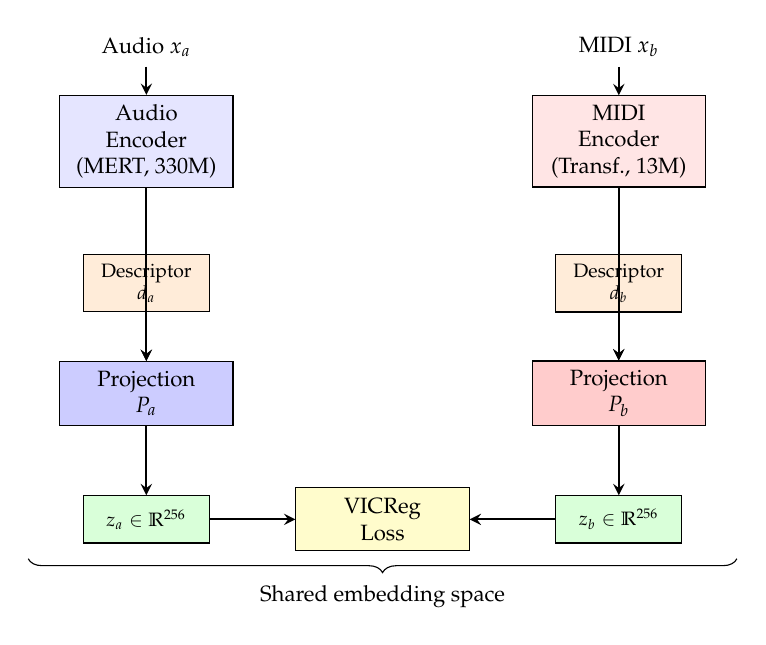
\begin{tikzpicture}[
    box/.style={rectangle, draw, minimum width=2.2cm, minimum height=0.8cm, align=center, font=\footnotesize},
    smallbox/.style={rectangle, draw, minimum width=1.6cm, minimum height=0.6cm, align=center, font=\scriptsize},
    arr/.style={->, thick},
    >=stealth
]
% Audio side
\node[box, fill=blue!10] (ea) at (-3, 0) {Audio\\Encoder\\(MERT, 330M)};
\node[smallbox, fill=orange!15] (da) at (-3, -1.8) {Descriptor\\$d_a$};
\node[box, fill=blue!20] (pa) at (-3, -3.2) {Projection\\$P_a$};
\node[smallbox, fill=green!15] (za) at (-3, -4.8) {$z_a \in \mathbb{R}^{256}$};

% MIDI side
\node[box, fill=red!10] (em) at (3, 0) {MIDI\\Encoder\\(Transf., 13M)};
\node[smallbox, fill=orange!15] (dm) at (3, -1.8) {Descriptor\\$d_b$};
\node[box, fill=red!20] (pm) at (3, -3.2) {Projection\\$P_b$};
\node[smallbox, fill=green!15] (zm) at (3, -4.8) {$z_b \in \mathbb{R}^{256}$};

% Input
\node[font=\footnotesize] (xa) at (-3, 1.2) {Audio $x_a$};
\node[font=\footnotesize] (xm) at (3, 1.2) {MIDI $x_b$};

% Loss
\node[box, fill=yellow!20] (loss) at (0, -4.8) {VICReg\\Loss};

% Arrows
\draw[arr] (xa) -- (ea);
\draw[arr] (ea) -- (pa);
\draw[arr] (da) -- (pa);
\draw[arr] (pa) -- (za);
\draw[arr] (xm) -- (em);
\draw[arr] (em) -- (pm);
\draw[arr] (dm) -- (pm);
\draw[arr] (pm) -- (zm);
\draw[arr] (za) -- (loss);
\draw[arr] (zm) -- (loss);

% Shared space bracket
\draw[decorate, decoration={brace, amplitude=5pt, mirror}] (-4.5, -5.3) -- (4.5, -5.3) node[midway, below=6pt, font=\footnotesize] {Shared embedding space};
\end{tikzpicture}
\caption{Architecture of the Phideus dual-encoder system. Each modality is encoded separately, guided by its descriptor, projected into a shared 256-dimensional space, and trained under VICReg loss. The descriptor injection point sits between encoder output and projection input.}
\label{fig:phideus_arch}
\end{figure}


\section{What counts as a descriptor in Phideus}


The word descriptor cannot do all the work by itself. Phideus needs three distinct terms. A descriptor is the informational structure injected into the model: what the model is being asked to attend to. A mechanism is the architectural route through which that structure enters: how it is injected. An arm is the concrete experimental combination of descriptor, mechanism, and training recipe. Keeping those terms separate is not pedantry. It is the only way to read the program without confusing content with route or route with full experimental condition.

For orientation, Table 11.2 below lists the descriptors themselves. Labels such as A4r or d4a4, which appear later in the chapter, do not name new descriptors but experimental arms built from those same descriptors under particular mechanisms.

That distinction clarifies several recurrent confusions at once. A4r is not a new descriptor; it is A4 under reverse cross-attention. Projection conditioning is not a descriptor; it is a mechanism for modulating the projection head. The canonical dual arm d4a4 is not a descriptor either; it is the experimental condition in which D4 guides the symbolic side and A4 guides the acoustic side. Once this vocabulary is fixed, the later results stop looking like a proliferation of unrelated labels and begin to read as controlled variations on a shared logic.

The descriptor-guided phase of Phideus was not the program's beginning. Earlier work explored denser and more literal representations of ratio structure: histograms of ratio distributions, sparse tokenizations inspired by acoustic fingerprinting, and exact matching schemes based on voting. Those experiments matter here only for one methodological lesson. Dense, temporally structured representations preserved enough organization to remain discriminative, while sparse matching and exact token logic tended to destroy the very cross-modal relation the program needed to learn. The move toward compact descriptors inside a learned embedding pipeline was therefore not arbitrary. It was the result of a prior elimination process.

Escalon 1 then made the descriptor problem operational without yet imposing a complete taxonomy over the whole program. It worked first with two pragmatic descriptors. D4 is a four-channel local interval descriptor on the MIDI side. For note \(i\), with MIDI pitch \(p_i\), it encodes the previous and next interval both in semitone and in octave-normalized log-ratio form:

$$
D4_i = \left[
\frac{p_i - p_{i-1}}{24},
\frac{p_{i+1} - p_i}{24},
\frac{\mathrm{clip}((p_i - p_{i-1})/12, -2, 2)}{2},
\frac{\mathrm{clip}((p_{i+1} - p_i)/12, -2, 2)}{2}
\right]
$$

A4 is the corresponding audio-side descriptor, computed from the temporal dynamics of log-magnitude in eight octave-like bands. If \(X_t(f)\) is the STFT magnitude at frame \(t\) and frequency bin \(f\), and \(B_b\) is octave band \(b\), then:

$$
\mu_b(t) = \frac{1}{|B_b|}\sum_{f \in B_b} \log(1 + |X_t(f)|),
\qquad
A4_t^{(b)} = \mu_b(t) - \mu_b(t-1)
$$

In implementation, these bandwise deltas are normalized and, when needed, interpolated to the target sequence length of the encoder side they guide. The important point for the present chapter is conceptual. D4 and A4 are descriptors. A4r is not a third descriptor but the arm in which A4 is injected through reverse cross-attention, and d4a4 is the dual arm in which D4 and A4 guide their respective modalities together. One descriptor is symbolic and explicitly local; the other is acoustic, broadband, and non-ratio in the strict sense. Together they were enough to establish the central closed result of the front, which Section 11.5 develops in full. But they did not yet settle the stronger question of natural harmony. A4 is spectrally rich without being a direct encoding of harmonic proportion, and D4 lives in a musically mediated interval space rather than in physically natural coordinates.

That is why the descriptor map of Phideus has to be read historically and experimentally rather than as a single universal family tree. Escalon 1 used D4 and A4 to prove that descriptor-guided cross-modal learning is a real and powerful mechanism. The retrospective music branch later reopened the question with A7, A9, and A10. Escalon 2 then introduced a new local taxonomy derived from the vocal oscillator itself. The point of the present section is not to flatten those moments into one scheme, but to make clear how they belong to the same program while preserving their different epistemic roles. Table 11.2 gives the compact map needed for the body of this chapter. The exhaustive inventory of descriptors, mechanism variants, and canonical arms belongs in Appendix C and in the companion methodological paper now in preparation, while the public Phideus repository carries the implementation-level detail.

\begin{table}[ht]
\centering
\caption{Inventory of descriptors across the Phideus program.}
\label{tab:descriptor_inventory}
\footnotesize
\begin{tabularx}{\textwidth}{@{}llclXX@{}}
\toprule
Front & Descriptor & Dim & Domain & What it encodes & HIT hypothesis \\
\midrule
Escalon~1 & D4 & 4 & MIDI & Local intervals & Symbolic relational structure \\
Escalon~1 & A4 & 8 & Audio & Spectral dynamics & Strong non-ratio control \\
Gate~9 & A7 & 12 & Audio & JI spectral ratios & Natural harmony retrospective \\
Gate~9 & A9 & 12 & Audio & JI spectral variant & Natural harmony retrospective \\
Gate~9/A10 & A10a--e & 6--32 & Audio & Recurrence-based ratios & Ontology-free relational encoding \\
\midrule
Escalon~2 & V4-lin & var & Speech & Linear $F_0$ ratios & Natural harmony in physical coords \\
Escalon~2 & V4-log & var & Speech & $\log_2 F_0$ ratios & Perceptual comparison \\
Escalon~2 & H-series & 12 & Speech & Harmonic amplitudes & Harmonic series structure \\
Escalon~2 & A4-16k & 8 & Speech & Spectral dynamics & Strong non-ratio control \\
\bottomrule
\end{tabularx}
\end{table}


\section{How descriptors enter the model: mechanism as variable}


If descriptors tell the model what kind of relation should matter, mechanisms determine how that guidance reaches the shared space. Phideus treats this not as implementation detail but as an experimental axis in its own right. A weak descriptor under one route may become productive under another. A strong descriptor may disappear if the route of injection is badly chosen.

Five mechanisms have structured the program so far. Concatenation appends descriptor values directly to encoder outputs:

$$
\tilde{h} = [h ; d]
$$

Cross-attention lets encoder features attend to descriptor tokens as an external source of guidance under the standard attention rule

$$
\mathrm{Attn}(Q,K,V) = \mathrm{softmax}\left(\frac{QK^{\top}}{\sqrt{d_k}}\right)V
$$

with \(Q=h\), \(K=d\), and \(V=d\). Attention bias perturbs self-attention more lightly, by modifying the attention logits from within the encoder without replacing the feature stream by descriptor tokens. Reverse cross-attention inverts the relation, using descriptor tokens as queries and encoder features as keys and values, so that \(Q=d\), \(K=h\), and \(V=h\). This proved especially useful in the retrospective music branch because it compresses long encoder sequences into a much smaller descriptor-guided interaction. Projection conditioning, inspired by FiLM, moves the intervention downstream and lets descriptor content modulate the mapping from encoder space into the shared space itself:

$$
h' = (1 + \gamma(d)) \odot h + \beta(d)
$$

This is the cleanest place in the program to see why descriptor and mechanism must not be collapsed. The same descriptor can behave very differently depending on whether it is concatenated, used as attention context, used as an attention query, or allowed to modulate the projection head late in the pipeline \parencite{vaswani_2017,perez_2018}.

The cleanest lesson of Escalon 1 is that route matters. Attention-based injection systematically outperforms simple concatenation, which means descriptor signal is not best understood as static side information pasted onto an embedding. It becomes productive when it is allowed to reorganize interaction among tokens. Projection conditioning adds a second lesson. Descriptor information can survive even when the intervention occurs at the end of the pipeline rather than at its beginning. The signal is therefore not tied to one privileged insertion point. It can work by reshaping token interaction early or by modulating the final projection late.

This distinction also stabilizes the reading of the chapter's own evidence. D4 and A4 answer the question of content. Concat, cross-attention, attention bias, reverse cross-attention, and projection conditioning answer the question of route. Arms such as d4a4, a4r, or d4-a4r belong to the level where both variables meet. Figure 11.2 schematizes the three most legible routes, while Appendix C and the methodological paper will carry the full implementation-level inventory. The later sections can then read results without collapsing these layers into one another.

\begin{figure}[ht]
\centering
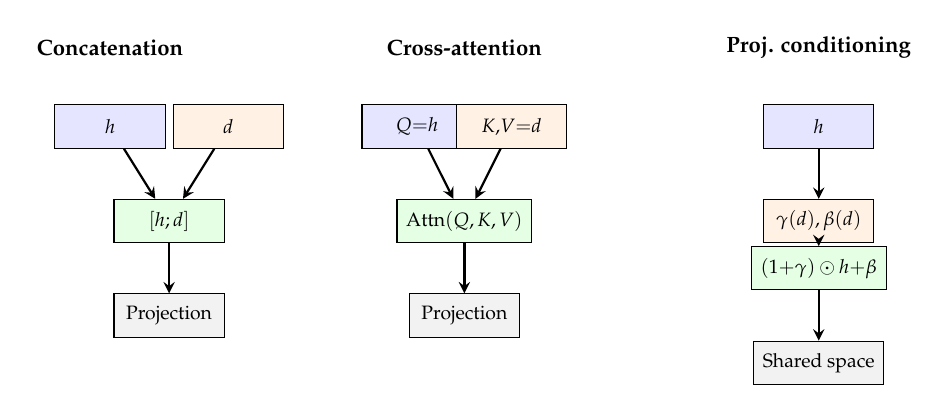
\begin{tikzpicture}[
    box/.style={rectangle, draw, minimum width=1.4cm, minimum height=0.55cm, align=center, font=\scriptsize},
    arr/.style={->, thick},
    >=stealth,
    every node/.style={font=\scriptsize}
]
% --- Concatenation ---
\node[font=\footnotesize\bfseries] at (-4.5, 2.2) {Concatenation};
\node[box, fill=blue!10] (c_h) at (-4.5, 1.2) {$h$};
\node[box, fill=orange!10] (c_d) at (-3.0, 1.2) {$d$};
\node[box, fill=green!10] (c_cat) at (-3.75, 0) {$[h ; d]$};
\node[box, fill=gray!10] (c_p) at (-3.75, -1.2) {Projection};
\draw[arr] (c_h) -- (c_cat);
\draw[arr] (c_d) -- (c_cat);
\draw[arr] (c_cat) -- (c_p);

% --- Cross-attention ---
\node[font=\footnotesize\bfseries] at (0, 2.2) {Cross-attention};
\node[box, fill=blue!10] (x_h) at (-0.6, 1.2) {$Q{=}h$};
\node[box, fill=orange!10] (x_d) at (0.6, 1.2) {$K{,}V{=}d$};
\node[box, fill=green!10] (x_att) at (0, 0) {Attn$(Q,K,V)$};
\node[box, fill=gray!10] (x_p) at (0, -1.2) {Projection};
\draw[arr] (x_h) -- (x_att);
\draw[arr] (x_d) -- (x_att);
\draw[arr] (x_att) -- (x_p);

% --- Projection conditioning ---
\node[font=\footnotesize\bfseries] at (4.5, 2.2) {Proj. conditioning};
\node[box, fill=blue!10] (f_h) at (4.5, 1.2) {$h$};
\node[box, fill=orange!10] (f_d) at (4.5, 0) {$\gamma(d), \beta(d)$};
\node[box, fill=green!10] (f_film) at (4.5, -0.6) {$(1{+}\gamma)\odot h{+}\beta$};
\node[box, fill=gray!10] (f_p) at (4.5, -1.8) {Shared space};
\draw[arr] (f_h) -- (f_d);
\draw[arr] (f_d) -- (f_film);
\draw[arr] (f_film) -- (f_p);
\end{tikzpicture}
\caption{Three descriptor injection mechanisms. \textbf{Left}: concatenation appends descriptor dimensions to encoder output. \textbf{Center}: cross-attention lets encoder features attend to descriptor tokens. \textbf{Right}: projection conditioning modulates the projection head via a learned affine transformation (FiLM).}
\label{fig:injection_mechanisms}
\end{figure}


\section{The central result: descriptor-guided cross-modal learning works}


The strongest closed result of Phideus remains the multi-seed validation of the canonical dual arm in Escalon 1. Across five independent seeds, d4a4 reaches a mean S of 84.1 percent with a standard deviation of 2.3 percentage points, while the unguided baseline D0 reaches 75.2 percent with the same standard deviation. The effect size is large, Cohen d = 4.50, and the distributions do not overlap: the weakest guided seed remains above the strongest unguided one. The result is not a fortunate run. It is a stable shift in the behavior of the system, and it must be read against the explicit pipeline just defined: descriptor content, route of injection, projection into shared space, and only then retrieval.

That retrieval advantage is supported by three causal lines of evidence. The first is inference-time ablation. When the A4 signal is zeroed at evaluation while keeping the trained weights fixed, performance collapses from 83.8 percent to 7.8 percent. The descriptor is not acting as decorative side information. The model depends on it. The second is parameter-matched degradation. Random, zeroed, or temporally shuffled substitutes fall back to the unguided band, leaving a causal gap of 9.4 percentage points between the real descriptor and the strongest degraded control. The advantage therefore comes from structured information rather than from added capacity alone. The third is pre-registration. Prediction matrices and admissible inference rules were written before the main readout, constraining interpretation before the relevant numbers were seen. That control does not make post-hoc reasoning impossible, but it sharply limits the most common forms of confirmation drift \parencite{pearl_2009}.

The evidence does not stop at retrieval. Cross-encoder alignment, measured by CKA, rises by roughly 82 percent in the guided condition, from 0.435 in D0 to as high as 0.794 in the best aligned arm \parencite{kornblith_2019}. At the same time, the descriptor-guided arms preserve roughly 29 percent more cross-modal information before the projection bottleneck. The descriptor is therefore not merely helping the model rank partners more effectively. It is altering the geometry through which both encoders are brought into relation.

Mechanistic evidence strengthens the same reading. Under projection conditioning, the best arm reaches 84.2 percent, the program's highest single-seed retrieval score. Even when only one side is conditioned late in the pipeline, the guided arm remains above the unguided control. Descriptor signal survives injection at the level of the projection head itself. This matters because it shows that the effect is not tied only to early token interaction. Guidance can remain operative all the way down to the final mapping into shared space.

The front also closes strongly at the level of discrimination difficulty. Descriptor-guided arms sustain hard-negative accuracy above 94 percent. These negatives come from the same musical piece at different temporal locations, so timbre, recording conditions, and style remain nearby while local identity changes. The model is not merely learning piece signature. It is learning temporal correspondence with fine resolution.

\begin{table}[ht]
\centering
\caption{Summary of convergent evidence, Escalon~1.}
\label{tab:escalon1_evidence}
\footnotesize
\begin{tabularx}{\textwidth}{@{}lllX@{}}
\toprule
Dimension & Test & Result & Interpretation \\
\midrule
Retrieval & Multi-seed replication & $84.1\% \pm 2.3$pp & Replicable advantage, $d = 4.50$ \\
Causal (ablation) & Inference-time zeroing & $83.8\% \to 7.8\%$ & Descriptor causally necessary \\
Causal (controls) & Parameter-matched degradation & $+9.4$pp gap & Information, not parameters \\
Geometric & CKA alignment & $+82\%$ & Representational reorganization \\
Information & Pre-projection retention & $+29\%$ & More cross-modal info preserved \\
Mechanistic & Projection conditioning & $84.2\%$ (record) & Signal survives deep in pipeline \\
Fine-grained & Hard negatives & $> 94\%$ & Temporal identity, not just piece \\
\bottomrule
\end{tabularx}
\end{table}

\begin{table}[ht]
\centering
\caption{Multi-seed replication of cross-modal retrieval, Escalon~1 ($n = 5$ seeds).}
\label{tab:escalon1_multiseed}
\footnotesize
\begin{tabular}{@{}lcccccc@{}}
\toprule
Arm & Mean $S$ & SD & Range & $\Delta$ vs D0 & Cohen $d$ & Sig. \\
\midrule
d4a4 & 84.1\% & 2.3pp & 82.0--86.4 & $+8.9$pp & 4.50 & $p < 0.001$ \\
d4-a4r & 81.2\% & 2.5pp & 78.4--83.4 & $+6.0$pp & 2.50 & $p < 0.01$ \\
a4r & 80.7\% & 1.9pp & 79.4--84.0 & $+5.5$pp & 2.63 & $p < 0.01$ \\
D0 & 75.2\% & 2.3pp & 71.8--77.4 & --- & --- & baseline \\
\bottomrule
\end{tabular}
\end{table}


\section{The second front: speech and electroglottography}


Escalon 2 poses a harder question than Escalon 1 because the modalities are no longer separated by notation versus acoustics. Speech is an airborne pressure wave. Electroglottography measures glottal contact through impedance. The event is shared, but the transduction is materially different from the start. Whatever cross-modal structure the model learns to use here has survived a genuine change in sensor physics.

That is why the unguided baseline matters so much. Under grouped bootstrap by speaker, D0 reaches 77.8 percent. On its own, that number already establishes something important: speech and electroglottographic traces share enough organization for a neural model to retrieve one from the other at a high level over structured candidate pools. Cross-modal structure in Phideus is therefore not confined to music, symbolic pairing, or aligned score metadata.

The first descriptor-guided pass over the vocal front was not framed as a failure hunt but as a mechanistic clarification. Twelve conditions were tested across descriptor families and routes of injection. None produced a defendable lift over D0 under the declared interpretive rules. That closes one easy reading and does something more valuable than a premature positive would have done: it shows that the front cannot be carried by weak wins under the current encoder regime. The existence claim is already secure at the level of the baseline. The open question is now more precise. Under what representational conditions does descriptor signal become legible in this harder domain?


\section{The discovery: representation organizes geometry}


The program's deepest finding is not exhausted by any single retrieval score. It is a structural discovery about what descriptor guidance does to representation.

The finding can be stated simply. Descriptor-guided models are not more linearly decodable than the unguided baseline. Ridge probes over the shared space return comparable or slightly weaker linear readout. And yet those same guided models show dramatically stronger cross-encoder alignment under CKA, along with higher information retention before the projection bottleneck. The descriptor does not simply add content that can be read out as one more feature. It reorganizes the shared geometry in which both modalities are brought into relation.

The descriptor does not enrich what the model knows. It reorganizes how the model relates what it already knows across modalities.

That distinction matters for the theory because it connects directly to the relational ontology developed earlier in the manuscript. If information is not exhausted by isolated substance but also lives in organized relation, then geometric reorganization is not a consolation prize below "real" performance. It is one of the most direct ways a system can show that a compact relational signal is constraining the field within which correspondence is learned. The effect disappears when descriptor content is degraded, which makes the reading stronger still. Ratio-based guidance is acting less like additive enrichment and more like geometric constraint.


\section{Phideus as constructive process}


Phideus is not merely observational. It is constructive. The program does not only ask whether ratio-based organization is present in signals. It builds models that attempt to learn under ratio-based guidance and then asks what changes in the resulting cross-modal space. That move matters because it turns a theoretical intuition into an engineering pressure test.

The constructive posture also imposes its own rigor. A descriptor may improve a model for reasons that do not validate the larger theory. It may regularize training, stabilize a bottleneck, or provide auxiliary structure without proving anything strong about harmony as such. The inverse can also happen: a theoretically important descriptor can fail because it was injected poorly, measured crudely, or tested under the wrong architectural comparison. Engineering utility and theoretical confirmation therefore cannot be treated as synonyms. Keeping them separate is not a weakness of the program. It is one of the conditions that makes the computational branch scientifically usable.

The next fronts extend that constructive logic without exhausting it. Escalon~3 will bring ratio into a domain where it is exactly specifiable, visible, and audible at once, creating the first experimental convergence with Beacon around Lissajous objects. Escalon~4 will ask whether the same general question can survive outside acoustics in cardiovascular physiology. Phideus can make harmonic hypotheses operational, but it cannot close the entire phenomenon from inside computation alone. The next chapter takes up the complementary task: what becomes visible when the same problem is probed through sustained acoustic fields, embodied response, and acoustic-physiological experience.


\section{Experimental implications of the activation conjecture}

Chapter~10 matters here because it sharpens what a computational probe should ask. If storage and retrieval are formally distinct, then a learned latent space should not be tested only with the same relational logic that helped stabilize it. It should also be tested with queries that challenge the space without simply collapsing into arbitrary noise. In practical terms, that means Phideus can compare integer-ratio probes, consonant neighborhoods, and $\varphi$-offset or noble-number perturbations as different ways of asking what a learned manifold preserves, when it locks, and when it becomes newly readable.

The point is not to turn Phideus into a golden-ratio machine. The point is to give the computational branch a sharper family of contrasts. A ratio-guided descriptor may help organize storage-like regularity in the latent space. A $\varphi$-offset query may help reveal whether that organization can be activated, traversed, or read without being overwritten by the same commensurate logic that produced the lock in the first place. That distinction creates a more exact experimental vocabulary for the fronts already named in this chapter, especially where the object is explicitly geometric or phase-bearing.

\chapter{Harmonic Beacon: The Experiential Probe}

\epigraph{\emph{It is not a sound object. It is a field.}}{}



\section{What the Harmonic Beacon is}


If Chapter 11 asked what becomes visible when harmonic hypotheses are made computational, this chapter asks what becomes visible when they are made physical, acoustic, and experiential. The Beacon is the experiential probe of HIT. It is a device built to generate a sustained harmonic field rather than an isolated sound event, and to do so under conditions precise enough that the resulting field can be treated as an object of investigation rather than as an atmospheric effect.

That distinction matters from the start. The Beacon is not a metronome, because its point is not periodic marking. It is not a drone, because the field it produces is internally structured rather than spectrally flat. It is not a sound bath, because its organizing principle is not immersion alone but sustained harmonic proportion. A motor excites a string continuously, and the instrument holds open a dense pattern of interacting partials that would otherwise collapse as soon as the note decayed. What the listener encounters is not a single pitch extended in time but a living interference field.

Operationally, the Beacon begins with a resonant source, an excitation method, a tuning procedure, and a room. In the earliest configuration the source is a guitar string coupled to a resonant body, and the excitation is a motor that keeps the system vibrating continuously instead of allowing a plucked event to die away. Later generations replace or complement that source with tuning forks, piezoelectric actuators, oscillator banks, and live networked outputs, but the logic remains the same. A harmonic field is sustained, tuned by coherence of the resulting interference pattern, and then probed through listening, biosignal capture, or visible pattern formation. The object of study is therefore not a recorded sound file. It is a physically maintained acoustic condition.

The reports surrounding that field are strikingly consistent. Listeners speak of melodies, choral textures, bagpipes, voices, and other organized sounds that are not explicitly present in the source. The useful term here is harmonic pareidolia. The point is to treat those perceptions as situated readings that emerge within a highly structured acoustic field rather than as a single fixed content that the source would simply contain in advance. The field is structured enough to sustain recognition and open enough to remain underdetermined.

That is why the Beacon matters for HIT. It provides a controllable source of natural harmonic organization in a register that computation alone cannot settle: embodied exposure to a sustained acoustic field. Phideus can test what ratio-guided structure does inside representation. The Beacon tests what a harmonic field does when it occupies a room, meets a body, and becomes part of an experienced environment. The chapter that follows is therefore not about a device in isolation. It is about the construction of an instrument through which the theory can be probed in physiological and experiential terms.

\begin{figure}[ht]
\centering
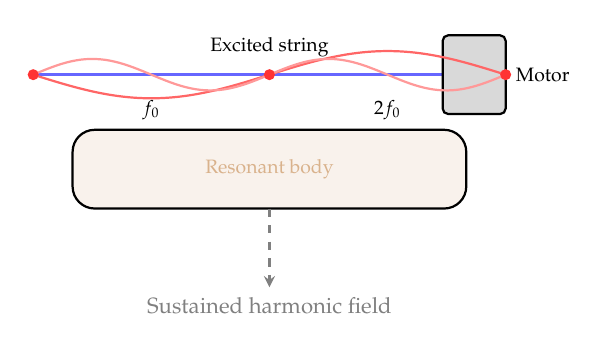
\begin{tikzpicture}[
    >=stealth, thick,
    every node/.style={font=\footnotesize}
]
% Guitar body outline (simplified)
\draw[rounded corners=8pt, fill=brown!10] (-2.5, -0.5) rectangle (2.5, 0.5);
\node[font=\scriptsize, text=brown!60] at (0, 0) {Resonant body};

% String
\draw[very thick, blue!60] (-3, 1.2) -- (3, 1.2);
\node[font=\scriptsize, above] at (0, 1.3) {Excited string};

% Motor
\draw[fill=gray!30, rounded corners=2pt] (2.2, 0.7) rectangle (3.0, 1.7);
\node[font=\scriptsize, right] at (3.0, 1.2) {Motor};

% Standing wave pattern
\draw[red!60, thick, samples=100, domain=-3:3] plot (\x, {1.2 + 0.3*sin(180*\x/3)});
\draw[red!40, thick, samples=100, domain=-3:3] plot (\x, {1.2 + 0.2*sin(360*\x/3)});

% Nodes
\foreach \x in {-3, 0, 3} {
    \fill[red!80] (\x, 1.2) circle (2pt);
}

% Labels
\node[font=\scriptsize, below] at (-1.5, 1.0) {$f_0$};
\node[font=\scriptsize, below] at (1.5, 1.0) {$2f_0$};

% Arrow: sound field
\draw[->, dashed, gray] (0, -0.5) -- (0, -1.5) node[below] {Sustained harmonic field};
\end{tikzpicture}
\caption{Schematic of the Beacon Guitar (first generation). A motor continuously excites a string coupled to a resonant body, sustaining a dense interference field of interacting partials rather than a decaying plucked event. Harmonic nodes are marked along the string.}
\label{fig:beacon_device}
\end{figure}


\section{Principle of operation: the harmonic gravitational field}


The Beacon is physically simple and experimentally demanding. A string under continuous excitation does not present only a fundamental. It presents the full harmonic series at once, with amplitudes and beat patterns shaped by the material properties of the string, the excitation point, the resonant body, and the room in which the instrument sounds. Classical acoustics has long treated that problem as one of coupled source, resonator, and field rather than isolated pitch production \parencite{rayleigh_1877, benade_1973, fletcher_1996}. The motor's function is not decorative automation. It converts an event that would normally decay into a sustained field in which the interaction among partials can be held open long enough to become perceptible, measurable, and tunable.

At the most compressed level, the harmonic logic can be written as:

$$
f_n = n f_0
$$

and the resulting field as:

$$
s(t) = \sum_{n=1}^{N} A_n \cos(2 \pi n f_0 t + \phi_n)
$$

where the amplitudes and phases are shaped by the source, the excitation geometry, the resonant body, and the room. The Beacon does not isolate one member of that series. It sustains a field in which several members remain simultaneously active and mutually constraining.

The central operation is therefore not "play a frequency" but stabilize a proportional field. Tuning is not performed by matching the system to an abstract external standard. It is performed by moving the excitation until the interference pattern becomes maximally coherent. In practice that coherence can be checked by ear, by laser, or by cymatic visualization. The criterion is not pitch purity in the narrow sense. It is the quality of the pattern generated by the interaction among partials.

That tuning operation can be written schematically as:

$$
\theta^* = \arg\max_{\theta} C(\theta)
$$

where $\theta$ stands for the tunable configuration of the setup and $C(\theta)$ stands for the coherence of the resulting pattern. The point of the formula is not to pretend that the Beacon already has a closed scalar metric for every installation. It is to make the operational criterion explicit: the target is the most coherent field the configuration can sustain, not the nearest approximation to an external equal-tempered pitch.

The metaphor of a harmonic gravitational field should be read in that concrete sense. When the system is near the right tuning, it does not merely sound different. It feels as if nearby organization is being pulled into a more stable relation. When the tuning drifts, the field becomes less inhabitable and the interference pattern loses coherence. The metaphor is useful because it captures a basin-of-attraction structure. The Beacon constructs a highly organized acoustic condition under which harmonic stability and instability can be experienced, interpreted, and worked with as differences in constraint.

That construction connects directly to earlier chapters. Chapter 4 described consonance as functional relation rather than isolated property. Chapter 8 described harmonic organization as a problem of efficient coordination under constraint. The Beacon translates those claims into a physical setup. It produces a field in which the difference between stable and unstable proportion is not only thinkable but experientially accessible.


The room is part of the experiment. The Beacon field interacts with surfaces, volume, air column, and placement. Each room produces a situated version of the field. That is not a flaw to be hidden but a feature to be handled. The Beacon is not a transparent playback device whose environment should be treated as negligible. It is a probe in which source and space co-produce the acoustic condition under study.


\section{Evolution of the device}


The Beacon did not appear as a finished object. It evolved through successive generations, each of which solved one operational problem and exposed another. That history matters because it shows that the device is not an aesthetic artifact but a chain of engineering responses to experimental constraints: how to sustain the field, how to tune it repeatably, how to transport it, how to connect it to sensors, and how to separate what belongs to harmonic organization from what belongs to the material support that produces it.

The first generation was the Beacon Guitar. Its problem was also its strength: how to obtain a dense, continuous, physically resonant harmonic field rather than a short acoustic event. The solution was a motor-driven string coupled to a resonant body and tuned manually until the interference pattern stabilized. A key step in that tuning procedure was measuring the spectral profile of the instrument itself---the characteristic timbre of the resonant body---and then tuning the strings to natural-ratio intervals derived from their relation to that spectral signature rather than to an external equal-tempered standard. This version established the phenomenon and made the field effect undeniable. It also had the highest spectral richness of the line. But it demanded daily precision, constant retuning, manual skill, and a favorable room. In other words, the generation that produced the strongest field was also the least portable and the least forgiving.

The second generation, the Pico Robot, answered that fragility by moving toward struck tuning forks and related resonant elements. The question here was no longer only how rich the field could be, but how repeatably it could be produced without the tuning burden of the guitar configuration. The gain was robustness, portability, and easier deployment. The cost was a narrower harmonic palette and a different phenomenological character. What was gained in stability was paid for in spectral density and in the open, flowing character of the original string-based field.

A particularly productive line of exploration across the second and third generations has been the systematic study of the relationships among the first five natural harmonics ($1\!:\!2\!:\!3\!:\!4\!:\!5$). These ratios define the densest region of simple-integer relations and have repeatedly yielded some of the clearest interference structures in our practical work. Within the range explored so far, the same region has also tended to generate the most stable and geometrically distinct Lissajous figures, which is why it has become a natural meeting point between the Beacon's acoustic work and the visible-pattern exploration described below. The cover image of this book is itself a Lissajous figure traced from the simultaneous resonance of these five harmonics.

The third generation moved toward digital control. Here the problem was no longer local fragility but limited programmability and limited coupling to external systems. The response took two complementary forms. On one side, a bank of harmonically organized oscillators controlled through OSC, including a grid of 64 harmonic pads and routable synthesis targets. On the other, the same 64-pad control surface driving piezoelectric actuators that excite metal reeds at independently controllable frequencies, connected wirelessly via Bluetooth. The first form is purely digital; the second recovers the physical resonance of earlier generations while gaining the programmability and repeatability of digital control. Both forms made exact recall, remote control, and sensor coupling much easier. They also opened a path toward harmonic feedback systems in which other data streams can modulate the field in real time. But the move reopened a different methodological question: how much of the Beacon's distinctive effect belongs to harmonic organization as such, and how much belongs to the material behavior of a physically resonant source such as a string, fork, or resonant cavity?

The fourth generation, still emergent, extends the Beacon toward distributed and networked operation. In this regime the point is not only to build one device that sounds in one room, but to make a live Beacon available through app-based access, remote listening, and later networks of synchronized devices. The explicit design choice is important: the app is not conceived as playback of a canned recording, but as access to a Beacon that is sounding in real time somewhere in the network. At that point the Beacon stops being only a local laboratory instrument and starts becoming a platform. Methodologically, this changes what can be transported, what can be personalized, and what kind of collective or environmental evidence the system can eventually seek.

\begin{table}[ht]
\centering
\caption{Beacon device generations: evolution from laboratory instrument to distributed platform.}
\label{tab:beacon_generations}
\footnotesize
\renewcommand{\arraystretch}{1.08}
\begin{tabularx}{\textwidth}{@{}P{0.14\textwidth}Y Y P{0.10\textwidth}P{0.13\textwidth}@{}}
\toprule
Generation & Physical source & Problem solved & Porta\-bility & Spectral richness \\
\midrule
Beacon Guitar & String + resonant body, continuous motor & Produces dense sustained field & Low & Highest \\
Pico Robot & Tuning forks + compact resonators & Improves robustness and portability & High & Medium \\
Digital/OSC & Oscillator bank / piezoelectric actuators + 64-pad harmonic control surface & Enables repeatability and sensor coupling & Very high & Controllable \\
App/\newline Distributed & Live remote Beacon node, streaming & Extends device into platform & Universal & Configur\-able \\
\bottomrule
\end{tabularx}
\renewcommand{\arraystretch}{1}
\end{table}

\begin{figure}[H]
\centering
\begin{subfigure}[b]{0.48\textwidth}
    \centering
    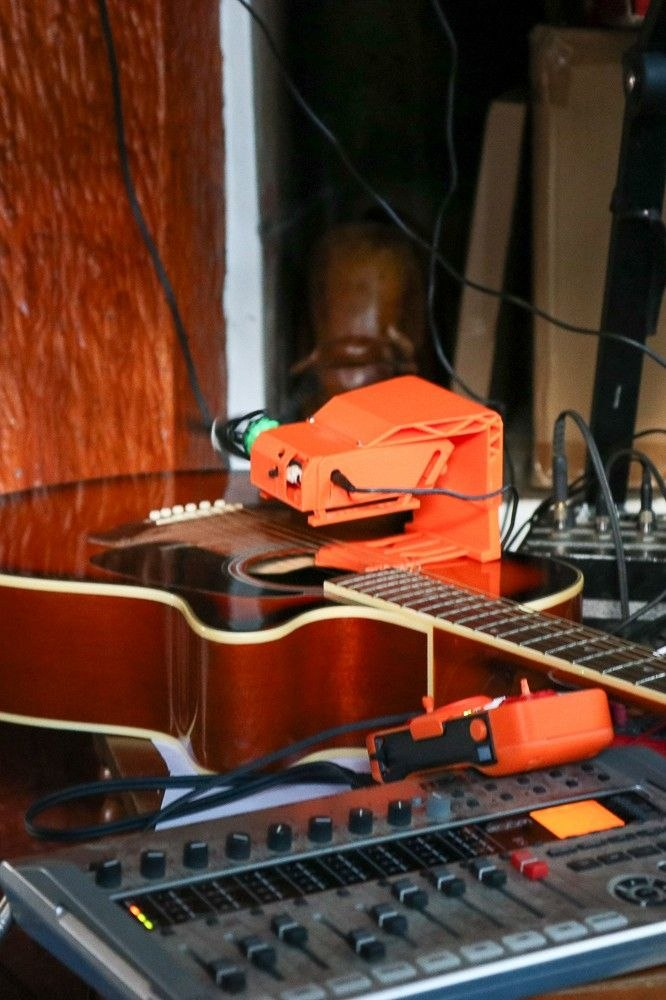
\includegraphics[width=\textwidth, height=5.5cm, keepaspectratio]{Beacon1_para_libro.jpg}
    \caption{Beacon Guitar (1st gen). Motor-driven string coupled to acoustic body.}
    \label{fig:beacon1}
\end{subfigure}
\hfill
\begin{subfigure}[b]{0.48\textwidth}
    \centering
    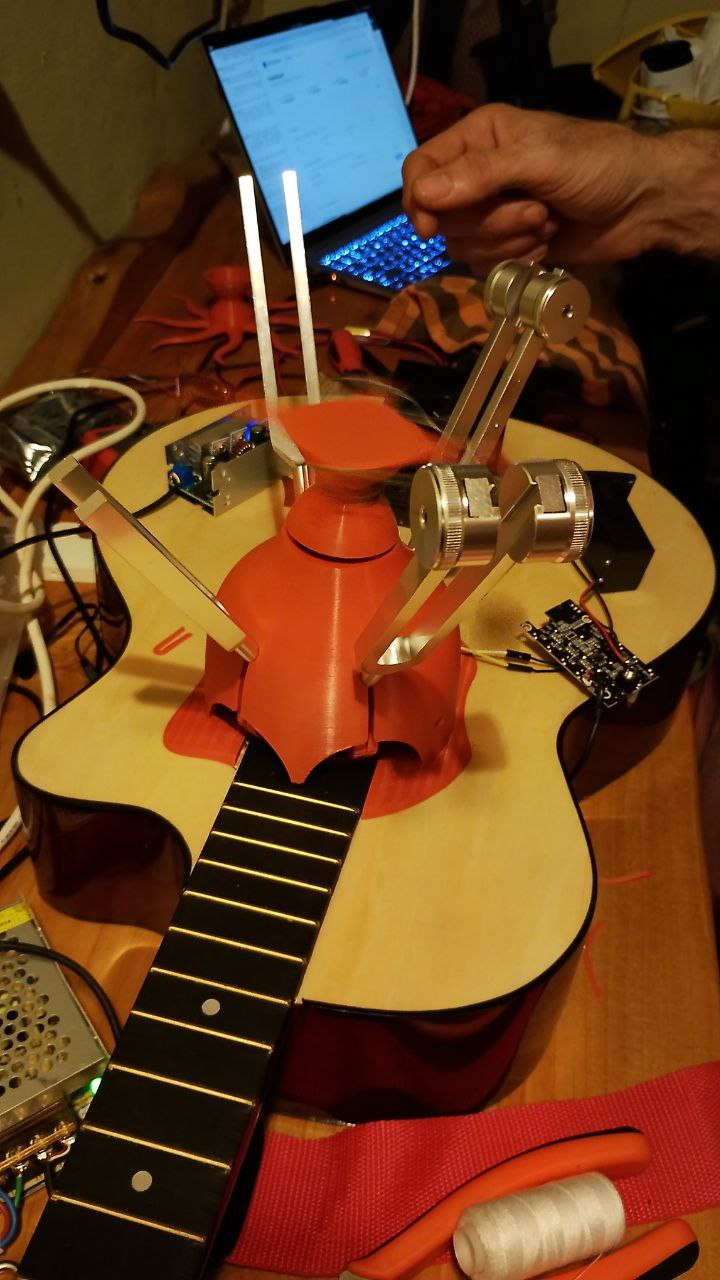
\includegraphics[width=\textwidth, height=5.5cm, keepaspectratio]{Beacon2.jpg}
    \caption{Pico Robot (2nd gen). Mechanical arms strike tuning forks on a guitar body.}
    \label{fig:beacon2}
\end{subfigure}

\vspace{0.5cm}

\begin{subfigure}[b]{0.48\textwidth}
    \centering
    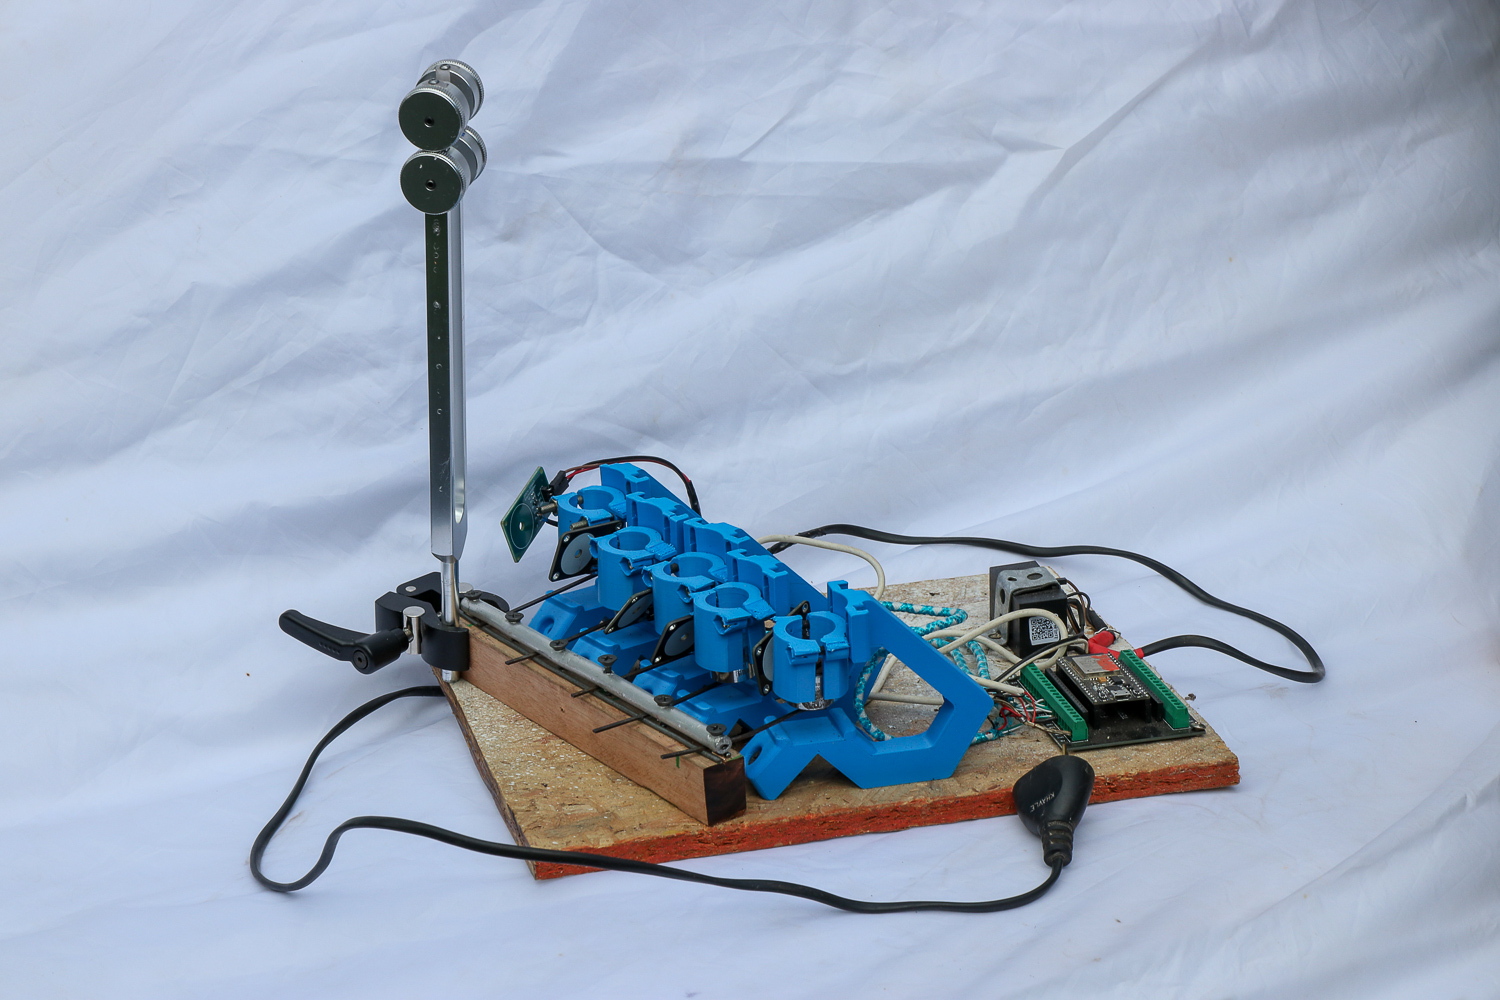
\includegraphics[width=\textwidth, height=5.5cm, keepaspectratio]{Beacon3-entero.jpg}
    \caption{Beacon 3 (3rd gen). Piezoelectric motors drive metal reeds, controlled wirelessly via Bluetooth from a 64-pad harmonic surface.}
    \label{fig:beacon3}
\end{subfigure}
\hfill
\begin{subfigure}[b]{0.48\textwidth}
    \centering
    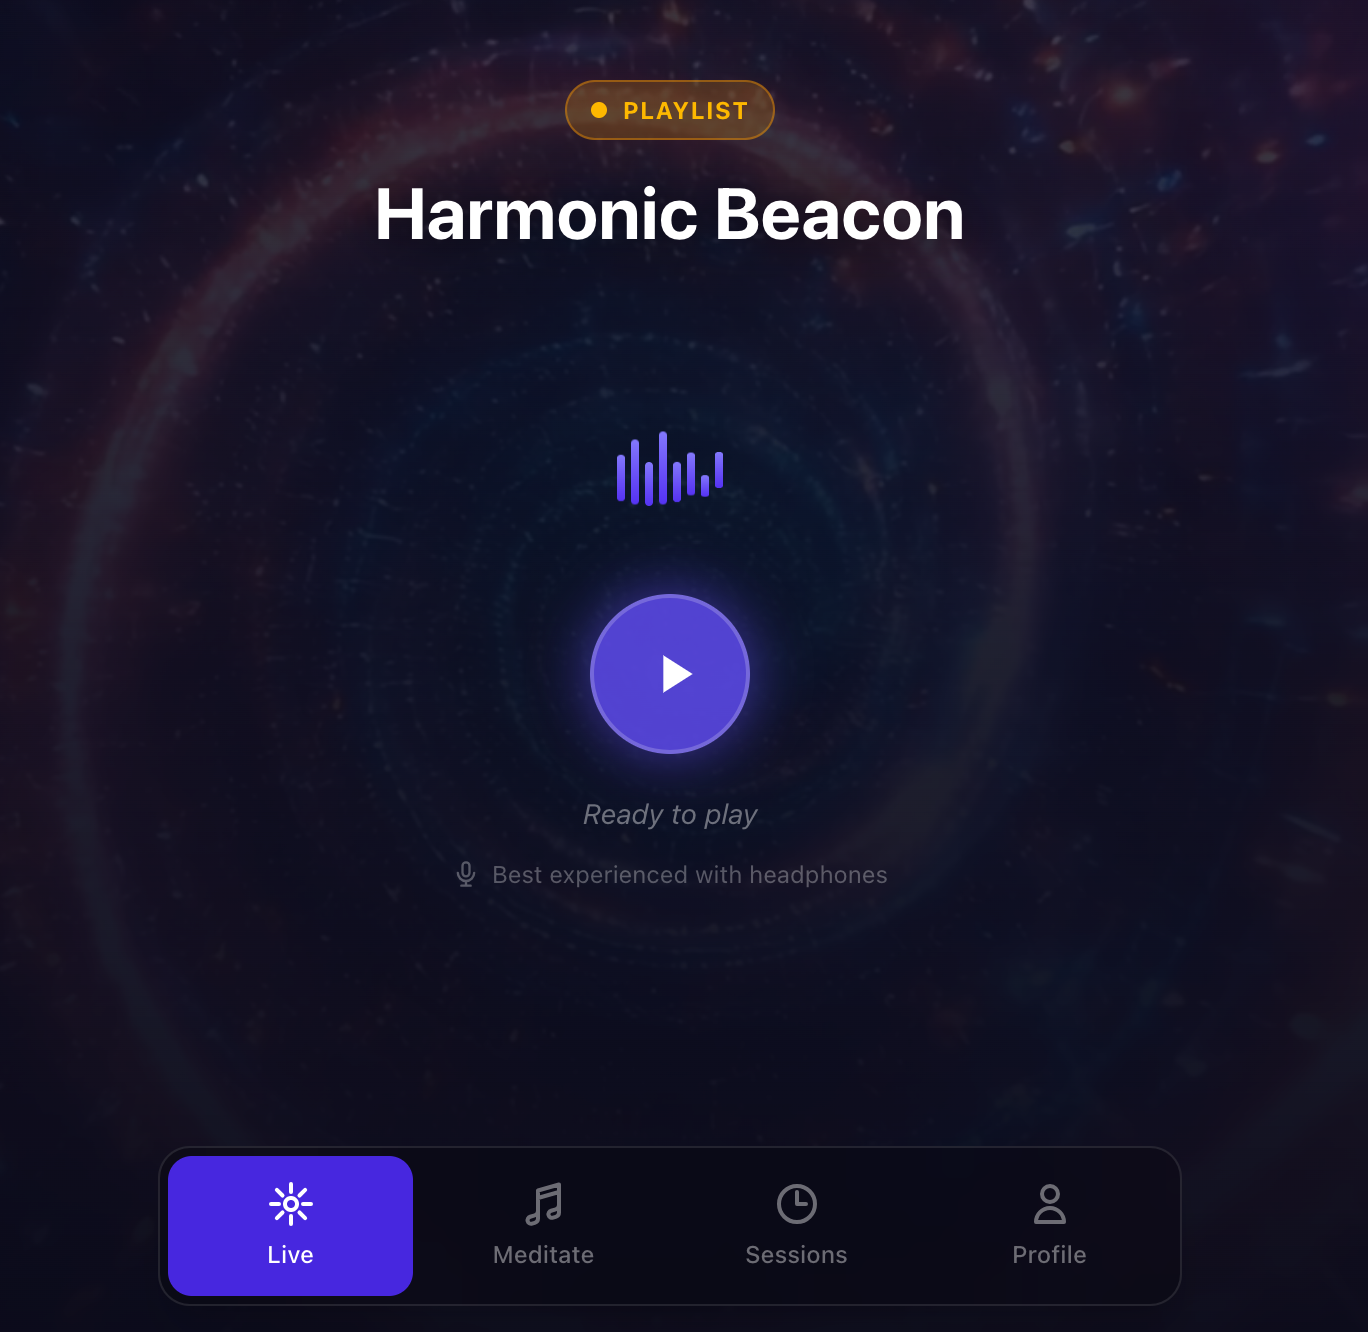
\includegraphics[width=\textwidth, height=5.5cm, keepaspectratio]{Beacon4-web-app.png}
    \caption{Harmonic Beacon app (4th gen). Live streaming interface for distributed access.}
    \label{fig:beacon4}
\end{subfigure}
\caption{Four generations of the Harmonic Beacon. The evolution moves from a fragile but spectrally rich laboratory instrument~(a) through increasingly robust and programmable configurations~(b,~c) toward a distributed platform accessible from any device~(d). Each generation solves one operational problem and exposes the next.}
\label{fig:beacon_generations}
\end{figure}


\section{Four experimental lines}


The Beacon opens four experimental lines. They do not all produce the same kind of evidence, and they are not equally mature. The first three share a common logic: expose a biological system to a controlled harmonic field and ask what can be measured, what shifts, and what sort of causal contrast could eventually adjudicate those shifts. The fourth line departs from that structure and turns the Beacon's instrumentation toward the systematic exploration of harmonic organization itself as a visible physical object.

The first line concerns biosignal reading and personalized calibration. Its experimental anchor is the Corazofono, a simple thoracic listening device composed of an acoustic coupler, a membrane, and a directional microphone whose output is read spectrally rather than only by ear. The goal is to estimate, under repeated speech prompts and controlled vocal tasks, the region in which each body concentrates its resonant energy most consistently, and to ask how that region should be read. The working observation is that thoracic resonance, breath, and cardiac pulsation do not distribute identically across subjects. That observation generates a precise research question. Is a harmonic field more effective when it is tuned to the subject's own resonant organization than when it is applied generically? The distinction between imposition and calibration is decisive here. If matching matters, then the body is not a passive receiver but part of the relation under study.

The second line measures physiological response under controlled exposure. Here the question is narrower and less speculative. Does exposure to a sustained harmonic field produce measurable changes in autonomic or cortical parameters relative to a baseline or matched control? Heart rate variability, respiration, EEG, and related signals belong to this line. The criterion is not whether the subject reports that the field was pleasant. Subjective report matters, but by itself it cannot discriminate harmonic organization from novelty, relaxation, expectation, or context. The line therefore aims toward pre/post designs and contrastive conditions in which the harmonic structure of the field, rather than sound in general, is what is being tested.

The third line concerns EEG-to-harmonics feedback: transforming the Beacon from a source of exposure into an interactive system in which measured neural dynamics modulate the harmonic field in real time. Because the electroencephalography hardware used in this line exports its readings via OSC, the same protocol already used for harmonic control, the technical path is direct: an application receives the EEG stream, translates its spectral content into frequency parameters, and routes those parameters to the Beacon's harmonic surface, so that the instrument responds in real time to the listener's own brain activity. A prototype of this application is currently under development.

What this makes possible is an experimentally legible feedback loop. Brain activity produces an electrical pattern; that pattern is read and translated into frequencies; those frequencies drive the Beacon; the Beacon's acoustic field reaches the body; and the resulting physiological response may in turn alter the next EEG pattern. The subject therefore receives continuous sensory feedback on a neural state that would otherwise remain imperceptible. The experimental question is whether that loop can support voluntary, intentional modulation---whether a person can learn to steer internal states by attending to the harmonic field that those states are themselves generating. If so, the Beacon would function as a brain--field interface: not a passive exposure device but an active channel through which cortical dynamics and acoustic organization constrain one another in real time. This line is the least mature of the four, but it marks the conceptual horizon of the Beacon program: harmonic organization is not only something to which a subject might respond, but also a candidate variable through which feedback itself might be structured.

The fourth line studies harmonic organization made visible. The Beacon's experimental work led independently to Lissajous figures as objects in which ratio becomes simultaneously audible, visible, and physically generable. This line uses a physical apparatus of controlled excitation, resonance tubes or vibrating membranes, mirrors, laser projection, and image capture to produce analog figures under repeatable conditions. In that respect it belongs to a longer experimental archive running from Chladni's vibrating plates to Jenny's cymatic investigations, where patterned excitation leaves stable traces in visible matter and geometry \parencite{chladni_1787, jenny_1967}. The point is to document how specific harmonic relations generate visible topologies in a pipeline where the source, the resonator, and the capture device are all part of the experiment. It matters because it pushes the Beacon beyond exposure studies and into the deliberate documentation of harmonic structure in visible form.

That exploration is being systematized through OpenClaw, the open-source agent framework used here for multi-agent orchestration and workflow decomposition.\footnote{Public repository: \url{https://github.com/openclaw/openclaw}. Multi-agent documentation: \url{https://docs.openclaw.ai/concepts/multi-agent}.} Within this line, OpenClaw coordinates experimental design, apparatus control, capture logic, and dataset construction as linked tasks rather than as isolated manual steps. Concretely, the OpenClaw agent is connected to the physical apparatus: it drives the excitation hardware, controls the mirror and laser projection geometry, and triggers a camera that photographs the resulting figure. The agent therefore does not merely plan experiments and organize data. It executes them: it selects a harmonic configuration, produces the corresponding physical figure, captures it, and registers the result as part of a growing dataset of ratio--topology correspondences. The practical effect is that the exploration of harmonic parameter space, capture conditions, and figure families can proceed as a structured research pipeline instead of a loose sequence of ad hoc interventions.

\begin{figure}[H]
\centering
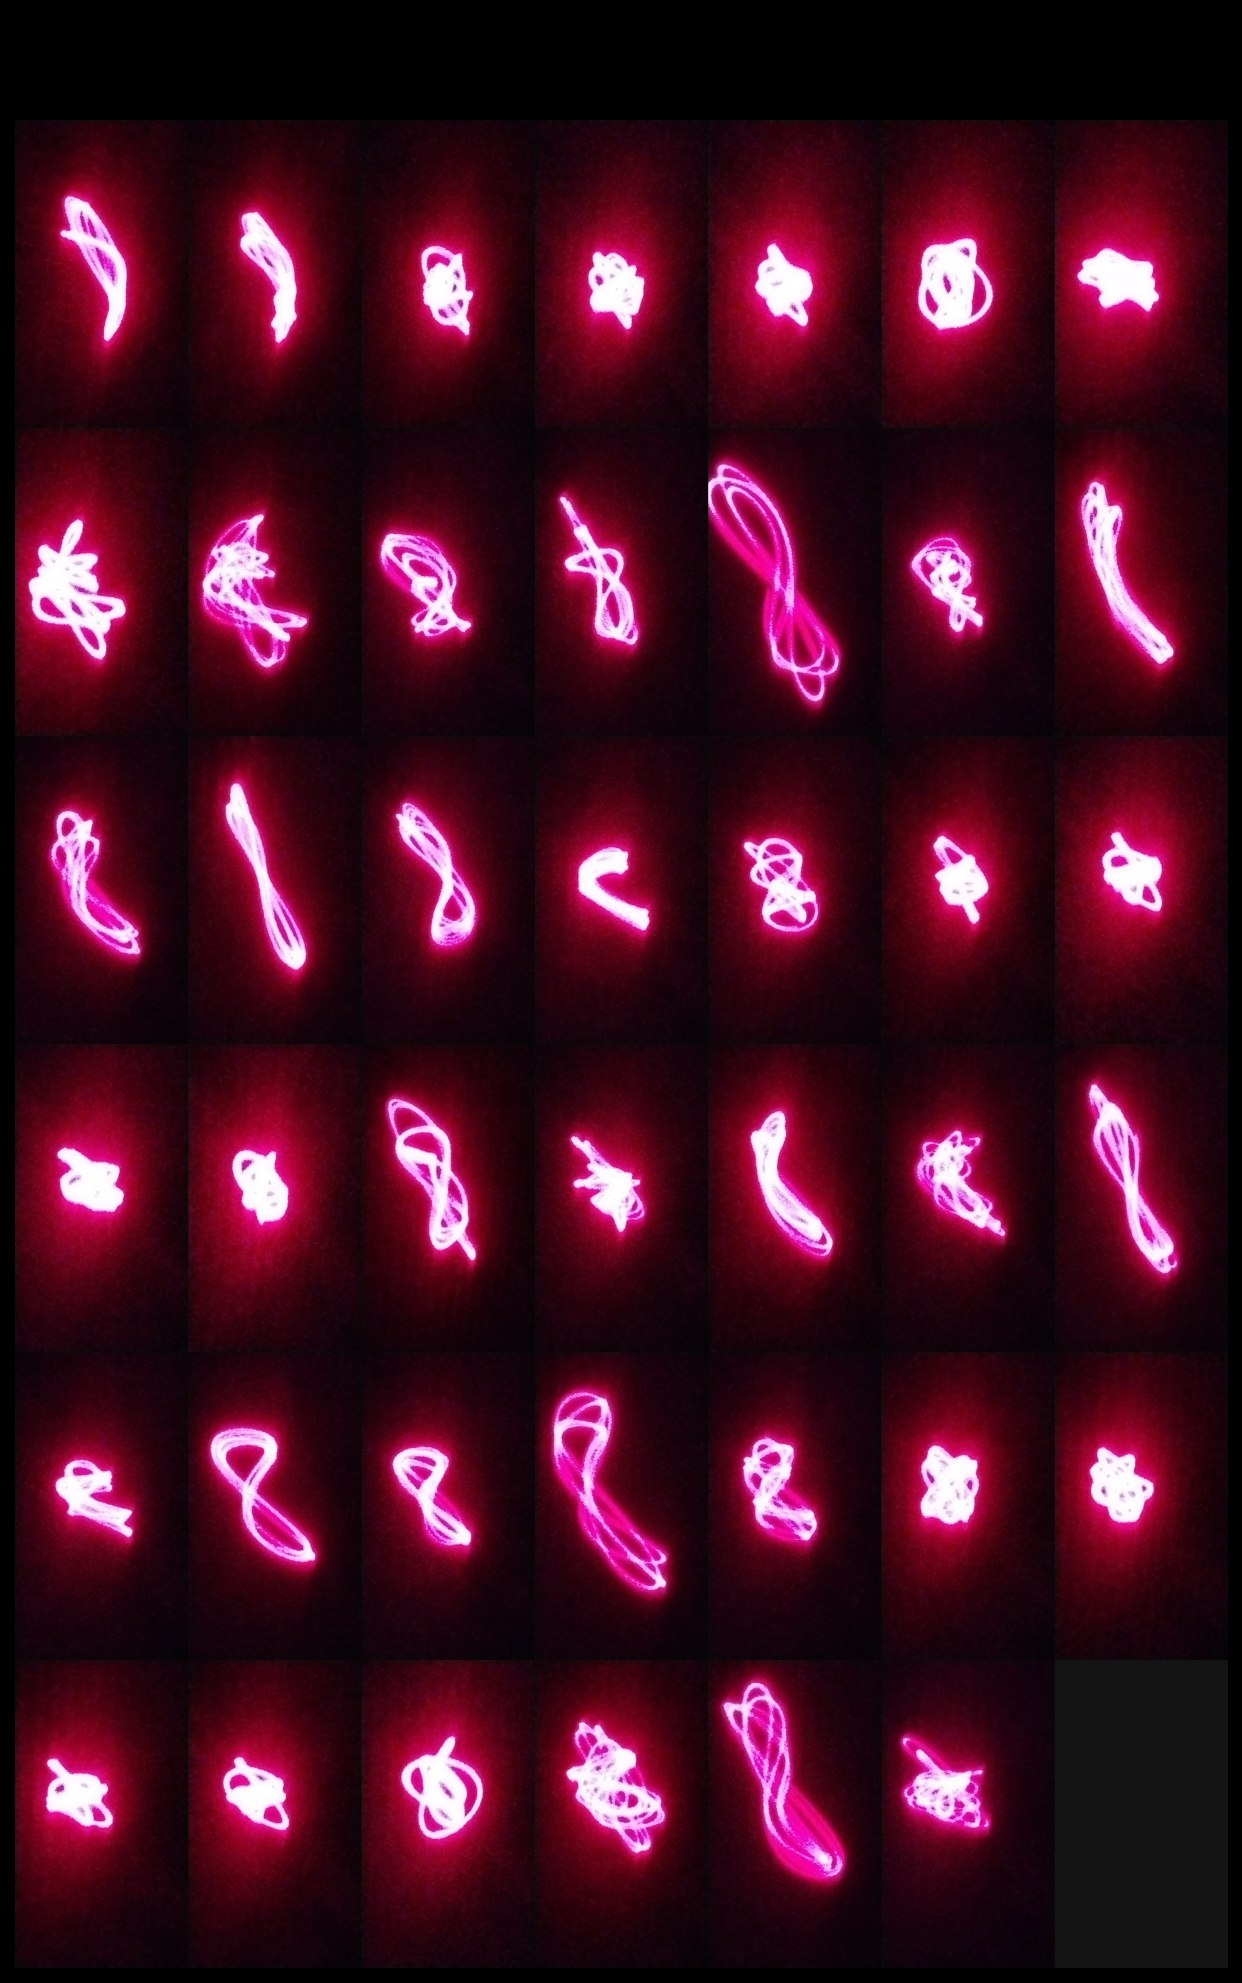
\includegraphics[height=0.58\textwidth, angle=90]{Openclaw-lissajous-exploration.jpg}
\caption{Sample matrix of Lissajous figures captured by the OpenClaw agent during autonomous exploration of harmonic parameter space. Each cell corresponds to a distinct frequency ratio produced by the physical apparatus and photographed by the capture system. The variety of topologies visible across the matrix illustrates how small changes in harmonic relation generate qualitatively distinct visible geometries.}
\label{fig:openclaw_lissajous}
\end{figure}

The dataset itself proceeds in two phases. In the first, synthetic sounds with known harmonic parameters generate analog figures through the physical apparatus. In the second, the sound source also becomes analog, yielding a fully physical pipeline from source to visible pattern. This line converges directly with Escalon 3 of Phideus. The computational branch reaches Lissajous figures because they provide deterministic control and exact parametric ground truth. The Beacon branch reaches them because sustained harmonic fields naturally produce visible ratio structure under physical resonance. The convergence is methodologically powerful precisely because the two probes arrive there for different reasons.

One consequence of the activation problem introduced in Chapter~10 is that not every informative perturbation of a harmonic field has to take the form of deeper consonant stabilization. A Beacon field can also be asked through offsets that are deliberately resistant to immediate locking. In practical terms, that opens the possibility of $\varphi$-offset or noble-number perturbations that function less as resting basins and more as activation signatures: brief, structured deviations that reveal how a field reorganizes without simply reinforcing the integer-ratio regime already being sustained. Whether such perturbations become experientially distinct, physiologically legible, or visually traceable is an open experimental question, but it now belongs explicitly to the Beacon program.

No quantified claim is carried by this section. The Beacon lines are named here as an experimental program, with unequal maturity and unequal evidential status. What matters at this stage is that each line asks a legible question, belongs to a shared architecture of evidence, and makes the Beacon more than an isolated device. It makes it a probe with a real research horizon.


\section{Personal Myth Projection}


Personal Myth Projection, or PMP, enters this chapter because Julian De La Reta, who develops this therapeutic practice, is also part of the broader team working on Beacon and Phideus. PMP is a psychotherapeutic technique developed by Julian De La Reta from the crossing of Jungian active imagination, Moreno's psychodrama, and Campbell's monomyth. It emerges from his own clinical and symbolic trajectory, while Beacon and Phideus emerge from the harmonic research program to which he also contributes. The relevance of PMP here is therefore not derivative but conjunctive: it opens a site where both lines of work can be explored together, where each may feed back into the other, and where PMP provides a structured setting in which the presence of a sustained harmonic field might matter for the accessibility and handling of deep psychic material. At the same time, the therapeutic process helps specify what kinds of effects the field may be making available and how those effects should be read.

Its first distinction is foundational. PMP operates on the side of vera imaginatio rather than fantasia. That means the session is not guided visualization, suggestion, or relaxation narrative. It is an encounter with images that arise with enough force to require agency, ethical involvement, and sustained attention from the subject. The patient is not asked to enjoy symbolic scenery. The patient is asked to remain in relation with material that may be difficult, resistant, or transformative.

The protocol gives that encounter a shape. A question is prepared. A warm-up reactivates bodily presence. The patient moves through the call, the threshold, the descent, the guardian, the crossing, the imaginal work itself, the return, and integration. Campbell's monomyth matters here not as a literary formula but as a map for psychic transition. Moreno matters because role reversal allows the subject to inhabit figures rather than merely describe them. Jung matters because the Self, the Shadow, and the Transcendent Function supply the theoretical grammar of the process. 

That independence has to remain explicit. Within this manuscript, PMP is being read primarily through the Jungian and psychodramatic lineage rather than through the categories of musicotherapy, sound healing, or entrainment. It belongs first to that symbolic and therapeutic architecture, and only secondarily becomes articulable with resonant devices. The reason to place it in this chapter is not to annex it to the Beacon, but to show that it opens a site in which the Beacon's field may become experimentally meaningful in a way that neither apparatus nor therapy produces alone.


\section{The PMP and Beacon conjunction: theoretical assembly and observations}


The conjunction between PMP and the Beacon can be stated through three formal nodes. All three are ways of rendering the research question legible.

The first is the problem of orientation. In Jungian terms, the Self is an orienting center that does not coincide with conscious command. In Beacon terms, the harmonic field functions as a non-discursive center of organization that is not reducible to a single tone or instruction. The correspondence is formal rather than exhaustive. The point is that both structures organize without operating through explicit command, even though they belong to different registers of experience and description.

The second node concerns process. The Transcendent Function names a movement in which opposed psychic contents are held long enough for a new relation to emerge. The harmonic process, as the Beacon stages it, likewise concerns the stabilization of relation under sustained proportion rather than under forced imposition. Again, the point is correspondence rather than collapse. It is a heuristic parallel that makes the conjunction thinkable without flattening one register into the other.

The third node is practical. PMP opens the descent toward difficult symbolic material. The Beacon can sustain the acoustic condition in which that work occurs. Repeated practice already suggests a stable pattern: under the sustained harmonic field, patients tend to remain in contact with deep material for longer, with less defensive contraction and with greater capacity to stay inside the process. The live question is therefore no longer whether something is happening at all, but how to describe, compare, and explain that difference with greater precision.

The observational basis at present is clinical, repeated, and already more structured than a single anecdotal impression. Across multiple applications with different people, the work has been accompanied by interviews, before/after tests, and therapeutic follow-up. The reports are remarkably convergent: access to deep material becomes more fluid, difficult imaginal confrontation can be sustained for longer, and post-session integration appears stronger. What remains open is not whether those effects are present for practitioners and participants, but how to formalize them under a stronger comparative protocol and what mechanism best explains them.

The negative demarcation matters as much as the positive one. PMP remains a therapeutic practice in its own right, and the Beacon is not exhausted by that therapeutic setting. The conjunction is therefore best read as an established field practice whose mechanism is still being clarified. What is under investigation now is not whether practitioners and participants experience a difference when both are brought together, but how that difference should be described, measured, and interpreted.


\section{HAT: Harmonically Aware Technology}


If the Beacon is the first localized instrument of this branch, Harmonically Aware Technology names its larger horizon. The idea is not one more device but a technological orientation in which spaces, instruments, and networks are designed with harmonic coherence in view. The provocation beneath it is simple: why should the built environment remain acoustically indifferent to the beings who inhabit it?

Taken seriously, that question does not begin in science fiction but in ordinary infrastructure. Routers select channels, appliances emit persistent vibration, rooms accumulate overlapping bands of noise, and houses become acoustic ecologies whether or not anyone designs them as such. HAT begins from the thought that those layers need not remain blind to harmonic organization. A harmonically aware house, router, or device would not merely emit less sound. It would situate its emissions, rhythms, and resonances in relation to the space and the bodies already inhabiting it.

A contemporary engineering frontier makes the same design intuition visible in another register. Jelin{\v{c}}i{\v{c}} and colleagues treat thermodynamic noise, locality, and hardware constraints as computational resources to be co-designed with the model itself \parencite{jelincic_2025}. The relevant lesson for HAT is clear: a technology becomes more interesting when it treats its material support as an active part of the computation rather than as an indifferent substrate. Extropic offers a serious neighboring example of physically situated design, while Beacon develops that orientation through resonant fields, bodily exposure, and acoustic control.

This is why the later generations of the Beacon matter. A distributed Beacon network, app-based access to a live sounding source, and OSC-based harmonic control already sketch the first pieces of such an infrastructure. The point is not playback but active configuration: a field can be generated, sustained, routed, adjusted, and eventually coupled to sensors that report something about the state of a room, a body, or a session. One possible horizon would therefore be a technological layer that does not simply broadcast energy into an environment, but listens to proportional organization and responds to it.

Read from that angle, Beacon and Phideus begin to divide a future architecture between actuator and sensor. Beacon points toward the generation of harmonic fields. Phideus points toward the discrimination of proportional structure across domains. If both lines continue to converge, one can begin to imagine something like an intuitive coprocessor: not a substitute for judgment, but a system able to register, compare, and respond to proportional organization in lived environments. A tentative name for that horizon would be PPU, a Proportional Processor Unity. The term is speculative and should remain so. It does not name a finished product. It names the possibility that future systems might process proportion itself as a meaningful layer of relation rather than as background noise.

That broader question prepares the next chapter. Once Phideus and Beacon are both in view, the issue is no longer what each probe can do in isolation, but what becomes thinkable when computational, physiological, and experiential branches begin to constrain and retroactively reshape one another.

\chapter{Phideus-Beacon Convergence}

\epigraph{\emph{The probes do not agree; they become answerable to one another.}}{}



\section{Two perspectives on the same hypothesis}


The central hypothesis of HIT, stated at its widest scale, is that harmonic or proportional organization matters for the structuring of information, for the stability of material systems, and for the ways living and symbolic processes hold together. Part V approaches that hypothesis through two probes built from very different materials. Phideus begins from paired datasets in which two domains register the same event, trains dual encoders and projection heads, compares descriptor-guided arms against explicit baselines, and asks whether ratio-based descriptions reorganize cross-modal representation. Beacon begins from the generation of sustained harmonic fields in physical space, calibrates those fields through resonant instruments and situated listening, and asks whether immersion in such conditions modifies bodily and experiential states. The conjunction with Personal Myth Projection adds a third site of observation: a structured therapeutic setting in which the presence of a harmonic field may matter for the accessibility and handling of deep psychic material.

Taken together, these probes open three distinct experimental registers. Phideus works in the computational register, where the question is whether proportional descriptions reorganize latent geometry under controlled variation. Beacon works in the physiological and experiential register, where the question is whether a sustained harmonic field modifies states, responses, and conditions of resonance in lived situations. PMP plus Beacon works in the psychological register, where the question is whether that same type of field changes the dynamics by which difficult symbolic material becomes accessible, stays open, and is later integrated. The registers are different, the instruments are different, and the vocabularies are different. What they share is a commitment to the same family of hypotheses: that harmonic organization carries structural consequences.

The asymmetry of maturity between the branches is real and informative. Phideus has closed positive evidence in its first completed front: replicated gains, causal controls, and measurable geometric reorganization. Beacon has a coherent device lineage, repeated observations, working protocols, and an experimental program that is already generating discriminating questions. PMP plus Beacon adds an established field practice with structured observation, interviews, before-and-after tests, and therapeutic follow-up across multiple applications. The open work there concerns formalization, comparison, and explanation. Convergence therefore works through mutual feedback and retroactive reshaping: heterogeneous probes reshape what becomes askable and legible in one another.


\section{The feedback loop: how each probe informs the other}


The two probes share a theoretical commitment and already feed each other in concrete ways. Phideus contributes a descriptor taxonomy, an explicit baseline-first discipline, and an adversarial culture of evaluation. The descriptor families developed there, from local interval structure to linear ratio profiles and harmonic amplitude summaries, extend naturally into the experiential setting. They can operate as harmonicity sensors for Beacon devices, helping tune a field, compare variants, or discriminate between natural, perceptual, and deliberately non-ratio controls. The same is true of the logic of comparison. The distinction between baseline and descriptor-guided arm, so central in Chapter 11, translates directly into Beacon design: one needs a field, a matched comparison, and a way of reading the delta rather than the isolated condition.

Beacon feeds Phideus through a different route. Corazofono practice suggests that each body presents a specific resonant organization and that this organization matters for how a sustained field is received. That observation pushes computational work toward descriptors that preserve individual spectral identity rather than washing it out into population averages. More broadly, Beacon keeps returning the computational branch to the room, the body, and the transduction chain. What Phideus measures in latent space remains connected to the fact that real signals come from situated bodies in real acoustic ecologies. That pressure widens the field of relevance of its descriptors and keeps its metrics tied to the environments from which those signals arise.

The feedback becomes more legible once PMP is added as a third vertex. Personal Myth Projection contributes a vocabulary of process that retrieval metrics and autonomic traces do not articulate by themselves. It asks a different question: what kind of access, symbolic descent, confrontation, or integration becomes more available under a sustained harmonic field? In that sense, the combined PMP-Beacon setting becomes another discriminating instrument, one able to say something about temporal process, psychic handling, and the structure of difficult material once the field is present.

The first direct experimental convergence between the two main probes occurs in the program's third phase, centered on Lissajous figures. Phideus approaches that object through synthetic generation with exact parametric ground truth. Beacon approaches it through analog capture, using physical resonance instruments, optical readout, and the multi-agent exploration architecture described in Chapter 12. Once the same proportional relations appear in both pipelines, a genuinely new question becomes available: whether the organization learned from synthetic data transfers to patterns captured from the physical world. The question treats both probes as two ways of reaching the same object and asks whether the structure detected on one side survives the passage to the other.

\begin{figure}[ht]
\centering
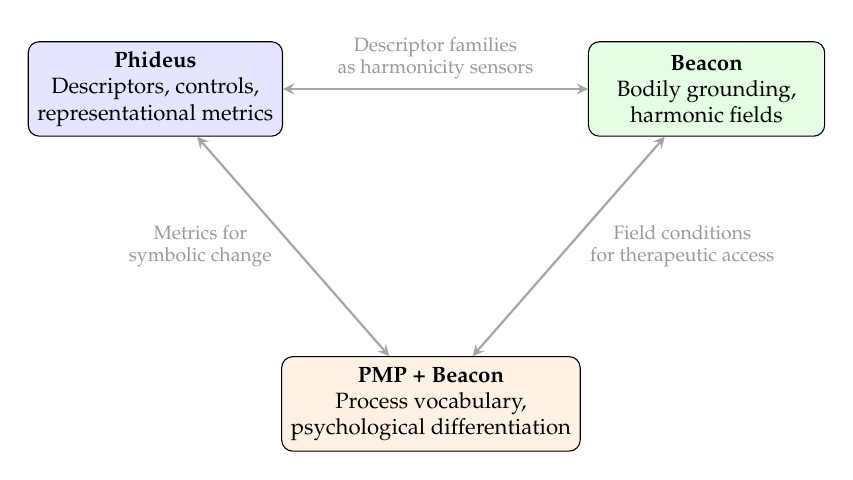
\begin{tikzpicture}[
    vertex/.style={rectangle, draw, rounded corners=4pt, minimum width=3cm, minimum height=1.2cm, align=center, font=\footnotesize},
    arr/.style={<->, thick, gray!70},
    lbl/.style={font=\scriptsize, text=gray!80, align=center},
    >=stealth
]
% Triangle vertices
\node[vertex, fill=blue!10] (P) at (-3.5, 0) {\textbf{Phideus}\\Descriptors, controls,\\representational metrics};
\node[vertex, fill=green!10] (B) at (3.5, 0) {\textbf{Beacon}\\Bodily grounding,\\harmonic fields};
\node[vertex, fill=orange!10] (M) at (0, -4) {\textbf{PMP + Beacon}\\Process vocabulary,\\psychological differentiation};

% Bidirectional arrows with labels
\draw[arr] (P) -- (B) node[midway, above, lbl] {Descriptor families\\as harmonicity sensors};
\draw[arr] (P) -- (M) node[midway, left, lbl, xshift=-4pt] {Metrics for\\symbolic change};
\draw[arr] (B) -- (M) node[midway, right, lbl, xshift=4pt] {Field conditions\\for therapeutic access};
\end{tikzpicture}
\caption{The Phideus--Beacon--PMP feedback triangle. Each vertex contributes a distinct register of evidence; bidirectional arrows indicate the type of feedback each pair exchanges. Convergence works through mutual constraint and retroactive reshaping, not ontological flattening.}
\label{fig:convergence_triangle}
\end{figure}


\section{The triangle: computational, physiological, psychological}


The conjunction of Phideus, Beacon, and PMP yields a triangle of registers. The computational register asks whether proportional descriptions reorganize representation between signals. Its evidence consists in retrieval deltas, causal ablations, baseline comparisons, and geometric reorganization under controlled variation. The physiological register asks whether immersion in a sustained harmonic field modifies measurable bodily states. Its evidence consists in calibration procedures, pre-and-post measurement, embodied observation, and the reproducible handling of acoustic conditions. The psychological register asks whether the same field changes the accessibility, duration, and integration of deep psychic material in therapeutic work. Its evidence consists in repeated field practice, session narratives, interviews, before-and-after tests, and structured clinical observation.

These registers are irreducible. Each speaks in its own instrument and vocabulary, and the passage between them takes the form of triangulation. Each register constrains and retroactively reshapes the others by forcing a translation of terms and by making weak readings harder to sustain. Computational evidence gains range when it meets bodily and experiential registers. Physiological and therapeutic patterns gain sharper form when they enter comparison with computational and experimental structure. The point of the triangle is to make these heterogeneous registers answerable to one another while preserving their differences.

The most interesting comparisons are therefore the ones that cross registers without erasing them. If the descriptors that most strongly reorganize computational space in Phideus were also the ones closest to the subject's thoracic organization in Corazofono readings, one would have a computational-physiological convergence of a specific sort. If a Beacon tuned to the subject's own resonant center produced more marked autonomic shifts than a generic harmonic field, personalization would become experimentally discriminable. If PMP sessions conducted under a tuned field showed systematically different access, duration, and post-session integration than comparable sessions conducted without that field, then the psychological register would enter a sharper relation with the physiological one. Some of these crossings already exist as repeated field observations. What remains is to formalize them under stronger comparative designs and to decide which descriptors, measurements, and protocols make each crossing most legible.

\begin{table}[ht]
\centering
\caption{Three registers of evidence in the Phideus--Beacon--PMP convergence.}
\label{tab:three_registers}
\footnotesize
\begin{tabularx}{\textwidth}{@{}llXlX@{}}
\toprule
Register & Probe & Question & State & Evidence \\
\midrule
Computational & Phideus & Do proportional descriptions reorganize cross-modal representation? & Closed positive & Causal controls + multi-seed replication \\
Physiological & Beacon & Does harmonic immersion modify bodily state? & Repeated observations & Calibration + pre/post measurement \\
Psychological & PMP + Beacon & Does a sustained harmonic field change access to deep material? & Formalization in progress & Interviews + before/after tests + clinical observation \\
\bottomrule
\end{tabularx}
\end{table}


\section{Vision: a network of Beacons, a landscape of harmony}


Read together, the three branches begin to divide a future architecture of sensor, actuator, and situated process. Phideus points toward harmonic sensing: the discrimination of proportional structure across domains, the comparison of descriptor families, and the ability to read whether organization is natural, perceptual, individualized, or deliberately degraded. Beacon points toward harmonic actuation: the generation, routing, and adjustment of sustained fields in rooms, bodies, and distributed networks. PMP contributes a structured setting in which the meaning of those fields is read through process, confrontation, and integration. This is also where Chapter 12's horizon of Harmonically Aware Technology becomes more concrete. A room, a device, or a network can be designed to sense, compare, and respond to the proportional organization of the environment it inhabits.

That horizon remains speculative and is already grounded in present lines of work. Later Beacon generations sketch a distributed infrastructure through live access, networked deployment, and OSC-based control. Phideus sketches the sensing side through descriptor-guided discrimination. Read together, they suggest the possibility of systems that process proportion as a meaningful layer rather than as acoustic residue. One tentative name for that horizon is PPU, a Proportional Processor Unity: an intuitive coprocessor for assisting the reading and modulation of proportional organization in lived environments. The question that opened Part V was whether the theoretical commitments of Harmonic Information Theory could survive contact with experiment. The answer now takes shape across a computational probe, a physiological-experiential probe, and a psychological field of practice that, together, make the phenomenon more observable and increasingly operable.



% --- PART VI ---
\part{Scope, Limits, and Future}
\chapter{What HIT Is Not}

\epigraph{\emph{Demarcation is not retreat. It is precision.}}{}


After the convergences assembled in Part V, a chapter of demarcation becomes necessary. A transdisciplinary program built around resonance, proportion, embodiment, and experiment is almost guaranteed to be read through categories that already circulate culturally: mysticism, reductionism, technological utopianism, acoustic romanticism, or total theory. The function of this chapter is therefore straightforward. It clarifies the type of object HIT studies, the kind of claims it is entitled to make, and the kinds of extrapolation that would distort the program rather than extend it.

HIT is not Pythagoreanism revived in scientific language. It does not treat pure ratio as an absolute substance or as a timeless metaphysical essence that silently governs all things from above. Ratios matter here because they can function as privileged relational constraints within concrete systems: oscillators, resonant cavities, vocal tracts, thoracic bodies, datasets, fields, rooms, and therapeutic situations. They matter through organization, not through purity. This is why the anti-essentialist guardrails developed earlier in the manuscript remain important here. Derrida and Nietzsche are useful at exactly this point. They remind us that origin, presence, and conceptual purity should not be reified too quickly into ontological guarantees \parencite{derrida_1967,nietzsche_1873}. HIT does not propose the ratio as hidden divine substrate. It proposes harmonic and proportional relations as experimentally and conceptually salient forms of organization.

For the same reason, HIT is not a naive universalism. Natural harmony is never simply "the same thing everywhere." Every system exposes its own affordances, thresholds, and local modes of coherence. The point made repeatedly across this manuscript, and sharpened by the empirical chapters, is that harmonic organization is local to the system in which it appears. A thoracic cavity, a forest soundscape, a room, a model architecture, a resonant instrument, and a Lissajous medium do not instantiate one invariant acoustic law in identical form. They instantiate families of proportional organization under different material and interpretive conditions. Cross-cultural work such as McDermott and colleagues on the Tsimane remains decisive here, not as a refutation of the whole program, but as a discipline against easy slides from recurrent structure to universal aesthetic law \parencite{mcdermott_2016}. HIT therefore does not identify recurrence with identical value, nor natural organization with one globally uniform perceptual response. Nor is it a theory of sound in the narrow sense. Sound and music remain one of its richest historical laboratories, but the framework is written for a wider family of oscillatory, resonant, and field-organized phenomena.

HIT is also not a closed theory. It is a research program. Lakatos remains the most useful name for that distinction: a program has a hard core, a revisable belt, a hierarchy of claims, and a future that depends on informative success and informative failure alike \parencite{lakatos_1978}. Popper remains equally important, not because falsifiability solves every philosophical problem, but because it helps block the temptation to protect the framework from contrast, replication, or adversarial test \parencite{popper_1959}. This manuscript therefore does not claim more than the current state of the evidence allows. Some fronts are stronger than others. Some results are closed and replicated. Others are protocol-bearing but still early. Others are established field practices whose comparative formalization is only now becoming sharper. The framework is strongest when those differences remain explicit. It weakens whenever every positive indication is made to carry the same theoretical weight.

This also means that HIT does not convert symbolic, spiritual, or experiential vocabularies into pseudo-physics. The manuscript can recognize that participants, practitioners, and traditions speak in terms that exceed the laboratory lexicon, and it can take those vocabularies seriously within their proper register. What it does not do is treat metaphor as mechanism or phenomenological language as if it were already a hidden causal model of matter. When this manuscript speaks of process, psychic depth, resonance, integration, or field, it does so under explicit epistemic discipline. Some of those terms belong to phenomenology, some to therapy, some to acoustics, some to computation. The work of HIT is to articulate and compare those registers without collapsing them into one another. In that sense the program is neither a scientistic purge of non-scientific language nor a refuge in claims that can never be tested. It is an attempt to coordinate heterogeneous vocabularies under shared standards of conceptual and experimental seriousness.

That discipline also situates HIT within a broader contemporary frontier rather than outside it. Analytic idealism, conscious realism, quantum interactive dualism, and Orch OR each reopen, in different and mutually incompatible ways, the relation between mind, matter, and field \parencite{kastrup_2017a,kastrup_2017b,hoffman_2008,stapp_2005,hameroff_2014}. HIT can converse with those programs without collapsing into any one of them. Its path remains different: it approaches the question through convergences around resonance, proportion, and experimentally tractable organization before drawing stronger ontological conclusions.

HIT is not reductionism. It does not reduce the cultural to the physical, the psychological to the computational, or the biological to the symbolic. The convergences assembled across Phideus, Beacon, and PMP plus Beacon are valuable precisely because they remain irreducible. Chapter 13 was explicit on this point: the computational, physiological, and psychological registers do not form a ladder of being and do not authorize a chain of automatic causal translation. They meet through triangulation, not through ontological flattening. This is equally important in the chapter's relation to Maturana and Varela. HIT is not autopoiesis applied. It does not claim that standing waves, harmonic fields, or patterns of interference are autopoietic in the strict biological sense. The distinction between organization and structure, the notion of structural coupling, and the idea of operational closure are used here as interpretive lenses that illuminate the problem of relation, not as licenses for identity claims between living systems and harmonic patterning \parencite{maturana_varela_1987}. The analogy is productive precisely because it remains an analogy.

HIT is not psychotherapy, and Beacon is not presented here as a clinically validated therapy ready to be prescribed as an alternative to established treatment. This matters especially now that the conjunction with Personal Myth Projection has entered the manuscript. PMP remains an independent psychotherapeutic technique developed by Julian De La Reta from its own lineage. Its articulation with the Beacon is a real field of practice and a real line of inquiry, but it should not be written as if the entire HIT framework collapsed into a therapeutic brand. The same caution applies on the technological side. The later discussion of HAT, distributed Beacon infrastructures, intuitive coprocessors, or a possible PPU is not a product brochure. These are horizon concepts: names for directions opened by the convergence of the program, not finished claims about devices already validated in the world.

None of these demarcations weakens the project. They make it more exact. They keep it from hardening too quickly into a metaphysics, an ideology, or a prematurely commercialized application. They also make room for a more honest account of limits. Some datasets remain small. Some results still depend on single-seed or low-N conditions. Some protocols are only now becoming stable enough for sharper comparison. Some branches of the program are more mature than others. Parncutt and Hair on critical debate in consonance research, and Di Stefano and colleagues on replicability problems, remain useful reminders that no frontier field gains anything by acting as if methodological fragility were a minor public-relations inconvenience \parencite{parncutt_2011,distefano_2017}. The value of HIT is not that it already possesses all the answers. The value lies in having coordinated a question strongly enough that the answers can now begin to differentiate, collide, and be tested under shared discipline.

\chapter{Open Questions and Research Agenda}

\epigraph{\emph{The future of the program is not one horizon but several distances.}}{}

After the convergences of Part V and the demarcations of Chapter 14, the program no longer needs another chapter proving that it is allowed to ask its question. What it needs is an agenda. Harmonic Information Theory now has enough internal structure that its open problems can be ordered rather than merely accumulated. Some belong to the immediate continuation of active fronts. Some extend those fronts into new domains or new instruments. Others remain theoretical or technological horizons whose relevance is already visible even if their implementation is still distant. Writing the agenda clearly therefore matters for the same reason that writing the evidence clearly mattered earlier. It prevents the program from flattening near tasks, medium-range expansions, and speculative futures into one undifferentiated field of desire.

That ordering also protects the chapter from two opposite distortions. One would be to reduce the future of HIT to laboratory housekeeping: more seeds, more runs, more datasets, more measurements, as if the problem were simply to scale an already finished framework. The other would be to jump too quickly from convergence to grand application or metaphysics. The agenda has to hold both pressures at once. It has to say what should be done next, what new domains can now be entered, and what stronger formalizations or architectures become thinkable only because the earlier work has made them intelligible. In that sense, the chapter is neither a backlog nor a manifesto. It is the point where a distributed set of findings becomes a programmatic map.


\section{Why an agenda is needed now}


The most immediate reason for an explicit agenda is that HIT has entered a new phase of internal asymmetry. Some results are already strong and comparative. Others are real but still thinly seeded. Others belong to experimental practices whose protocolization is only now becoming sharp enough for public articulation. Without an ordered agenda, those unequal maturities are too easily misread. A frontier with a living computational probe, an acoustic-physiological probe, and a psychological field of practice can begin to look either more finished than it is or more chaotic than it is. The chapter must therefore preserve a simple discipline: every task should be located at the scale where it actually belongs.

This is also why the agenda must be written as a sequence and not as an inventory. The first horizon is immediate and programmatic: open questions that can already be attacked within active fronts. The second horizon is expansive: new domains, new carriers, and new descriptor families that grow directly out of the current work. The third horizon is formal and technological: stronger mathematical articulation, broader theoretical synthesis, and possible architectures that become imaginable only once the first two horizons have been clarified. That hierarchy does not make the later horizons less important. It makes them readable without inflation.


\section{Immediate questions and programmatic next steps}


Some of the next tasks are close enough to the existing program that they should be described not as future dreams but as direct continuations of work already under way. The first is comparability itself. Where a front still depends on single-seed or low-seed results, multi-seed validation remains a priority, not because repetition is bureaucratic virtue, but because the strongest claims of HIT depend on distinguishing structural signal from accidental optimization. The framework has already insisted that observation, hypothesis, and inference must not be collapsed into one another. The immediate agenda simply applies that same rule to active fronts: what has been seen strongly enough to support a conclusion, what still needs broader validation, and what remains suggestive but not yet settled.

The clearest immediate question in that sense is now \texttt{Speech$\leftrightarrow$EGG}. The point of the foundation-encoder regime test is not merely to swap one backbone for a larger one. It is to ask whether the legibility of descriptor-guided structure depends in part on the regime of representation itself. If a frozen foundation encoder on the speech side makes the descriptor signal newly visible, then the negative or null result of earlier arms must be reread as a question about representational power and asymmetry, not only about descriptors. If it does not, the null becomes harder and more informative. In both directions, the task is valuable because it reduces ambiguity left by the second front rather than multiplying novelty for its own sake.

An equally immediate task remains on the retrospective side of Escalon 1. The distinction between descriptor and mechanism was one of the major clarifications of the current manuscript, and it still has to be closed as an experimental reading rather than left as a conceptual correction. The remaining work there is not to reopen the entire archive. It is to consolidate the descriptor-by-mechanism contrast tightly enough that later generalizations to new domains are not built on a confusion the program itself has already diagnosed.


\section{Phideus beyond the current fronts}


Beyond those immediate continuations, the most important medium-range expansion is the Lissajous line. It matters because it is the first domain in which ratio can be generated, seen, and measured under exact control while also becoming shareable across the computational and analog branches of the program. On the Phideus side, that means retrieval between \texttt{audio XY} and figure, recovery of generative parameters, new topological and geometric descriptors, and a direct comparison between rational and irrational sweeps. On the Beacon side, it opens the possibility of a captured analog dataset built from physically excited media. The long-term importance of this front lies in the fact that it brings a problem usually scattered across acoustics, geometry, optics, and signal analysis into a single object with deterministic ground truth and cross-probe accessibility.

The same front also reopens an older and harder question: how much of a visible or measurable pattern belongs to the medium, how much to the excitation, and how much to the interaction between them. That is why the inverse-nodal problem matters here. The task is not only to classify figures or recover ratios. It is to ask how far one can infer the structure of the system from the topology of the pattern it stabilizes, and where that inference begins to fail under drift, nonlinearity, or irrational forcing \parencite{pinasco_2021,maynard_1985}. Read that way, Lissajous is not a decorative side branch. It is a controlled arena in which the relation between proportion, topology, inference, and medium can be pushed far harder than in the current audio-only benchmarks.

Phideus also has to widen what counts as a descriptor. The recurrence family already points in that direction, but recent work on multifrequency oscillatory portraits suggests an even broader route. Bahuguna and colleagues show that the interdependence structure of oscillatory portraits can become a predictive object in its own right rather than a mere summary of signals after the fact \parencite{bahuguna_2025}. For HIT, that result matters twice. It offers a template for descriptor families that operate trial by trial on relational organization across bands or oscillators, and it suggests a complementary metric space for evaluation beyond retrieval alone. A learned representation could then be asked not only whether it retrieves the correct partner, but whether it preserves or reorganizes the oscillatory portrait of the phenomenon under controlled transformations.

Two additional expansions follow from that same logic. One is transfer: whether a model trained in one cross-domain regime carries anything useful into another. The other is domain shift beyond acoustics. The cardiovascular line and the structural-vibration line are both important because they test whether the descriptor-guided logic survives when the carrier changes. Chakraborty and colleagues' structural vibration dataset is especially useful in that respect because it shows that informative identity can be embedded in oscillation propagating through built structures rather than through air alone \parencite{chakraborty_2025}. If harmonic information is really about structured relation and not about sound as such, then the move into vibration fields, sensor arrays, and technical media is not a decorative expansion. It is one of the strongest tests of the framework's stated generality.


\section{Beacon and PMP+Beacon: from observation to protocol}


The Beacon agenda begins from a different maturity profile. Here the problem is less the absence of interesting effects than the need to stabilize protocols around observations that are already rich. The corazofono line needs exactly that kind of transition. What matters is no longer only that a thoracic resonant center seems individually detectable under guided production, but how to measure its variation, compare personalized against generic settings, and establish what changes under exposure and calibration. The same is true of the EEG-to-harmonics line. Its importance lies not in presenting a spectacular real-time loop for its own sake, but in asking whether physiological streams can become control surfaces for harmonic synthesis in ways that remain legible, repeatable, and interpretable.

The pareidolia line belongs to the same family of problems. It does not need to be defended as if the experience itself were illusory until an instrument redeems it. Nor should it be inflated into a finished theory of perception. What the agenda requires is a disciplined protocol for distinguishing spontaneous projection, structurally induced projection, field dependence, and individual variation. The same discipline applies to the contrast between personalized and generic Beacon configurations. If the field matters differently when it is tuned to the organization of a particular body or voice, then that difference has to be rendered protocol-bearing rather than left as a persuasive anecdote.

The Lissajous convergence reappears here in its analog form. The construction of a captured analog dataset through physically excited media, optical readout, and systematic exploration is important not only because it links Beacon and Phideus. It also forces the Beacon line to formulate its own standards of control, drift management, and reproducibility. That makes it one of the strongest candidates for a shared experimental object across branches of the program.

The \texttt{PMP+Beacon} agenda begins from another asymmetry again. Here there is already repeated practice, interviews, before/after tests, and convergent observation; what remains underdeveloped is the comparative design capable of making those materials readable across cases. The central next step is therefore not to ask whether anything happens in sessions. It is to compare \texttt{PMP} alone with \texttt{PMP+Beacon} under conditions strong enough to say what changes in depth of access, sustained tension, symbolic elaboration, and later integration. That requires not only bio-signals and questionnaires, but also disciplined content analysis, judges blind to condition where possible, and a more explicit treatment of sample size and variation than the current practice alone can provide.

This is also where the language of registers matters again. A psychological field of practice cannot be reduced to physiology simply because physiology is measured alongside it, and symbolic transformation cannot be treated as noise because it resists easy quantification. The agenda is strongest when it keeps those registers distinct while still putting them into a shared protocol. That is the real task of \texttt{PMP+Beacon}: not to collapse therapeutic process into bio-signal, but to build a comparative architecture in which experiential, physiological, and symbolic change can be read together without being mistaken for the same type of evidence.


\section{Formalization and long-horizon technology}


The experimental agenda alone is not enough. HIT also needs stronger formalization of the concepts it has used to organize its evidence. The most obvious unfinished problem is harmonic efficiency itself. What kind of information is preserved, compressed, stabilized, or made easier to recover under simpler proportional relations? How much of that depends on the receiver, the medium, or the task? Questions of this sort connect the framework naturally to the free energy tradition, where the issue is not whether a system “likes” a field, but whether certain relations reduce corrective burden, prediction error, or coordination cost in ways that can be described without metaphysical inflation \parencite{friston_2010}. They also connect to biosemiotics, where the relation between sign, organism, and environment becomes relevant precisely when patterned differences begin to matter for coordination and action \parencite{hoffmeyer_2008,barbieri_2008}.

Another unfinished formal problem lies in the relation between structural coupling and mode locking. The analogy already plays an important role in the manuscript, but it still needs a more exact mathematical articulation. Can one formulate a metric of successful coupling that links the width of an Arnold tongue, the stability of a relational regime, and the properties of the receiving system without pretending that oscillators and organisms are the same kind of thing? The same question extends into the problem of autonomy and precariousness raised earlier in the manuscript: whether systems under different forms of fragility respond differently to the same harmonic field, and whether that difference can be made measurable without erasing the specificity of the organismic case \parencite{dipaolo_2005,maturana_varela_1987}.

On the side of descriptor design, Wang and colleagues' Harmonic Aggregation Entropy is useful precisely because it suggests a family of estimators that begin from consistency of relation rather than from isolated peaks or absolute magnitudes \parencite{wang_haagen_2025}. The point is not that Phideus should simply import that metric unchanged. It is that the space of possible descriptors is larger than interval summaries, spectral envelopes, or recurrence counts alone. Higher-order relational estimators, aggregation-based measures, and noisy-series harmonicity scores all point toward a richer future vocabulary for the computational branch.

The final horizon belongs to technology, but only after the experimental and formal questions have been differentiated clearly enough to support it. If Phideus continues to develop as a proportional sensor and Beacon as a proportional actuator, then the possibility of a more integrated architecture becomes newly legible. That is the point at which the name \texttt{PPU} can enter without sounding either premature or empty. A Proportional Processor Unity would not name a finished machine. It would name the horizon in which reading, comparing, and modulating proportional organization become coupled operations within one system. For now that remains speculative, and it should remain speculative. But it is no longer unintelligible. The agenda has made it sayable. The next chapter can therefore ask a different kind of question: not what must still be investigated, but what kinds of derivation, application, and public consequence might follow if this program continues to mature.

\chapter{Applications and Derivations}

\epigraph{\emph{What follows is not closure. It is a larger field of consequences.}}{}

If Chapter 15 orders the future as agenda, this final chapter asks a different question. Given what the program has already made observable, protocol-bearing, and partially formalizable, what kinds of derivation become reasonable? The distinction matters. A derivation is not the same thing as a finished application, and it is not the same thing as a speculative dream. It names a consequence that can already be thought from the current state of the work, even if the final form of that consequence is still open. Writing the chapter in those terms allows HIT to speak publicly about possible uses, designs, and consequences without pretending that every line of extension is equally mature.

That distinction also keeps the chapter from collapsing into two opposite genres at once. On one side lies the temptation of the brochure: to move too quickly from experimental convergence to product language, clinical promise, or technological solutionism. On the other lies the temptation of excessive modesty, in which every derivation is treated as too premature to state clearly. Neither extreme is useful. The program has already produced enough structure to say more than "more research is needed," but not enough to present its consequences as if they had already been stabilized into validated interventions. The point of the chapter is therefore to order derivations by epistemic distance: what can already be approached instrumentally, what belongs to active design problems, and what remains a horizon of long-range articulation.


\section{What a derivation means here}


The first derivations of HIT are close to instrumentation rather than to ideology. They begin where proportional organization can already be read as a candidate variable under explicit conditions. In that sense, the chapter is not a departure from the empirical core of the book. It is an extension of it. Once one has shown that harmonic and proportional relations can matter for retrieval, geometry, bodily calibration, physiological response, or symbolic handling, the next step is to ask where such relations can become legible in public practice. The strongest answer is never "everywhere." It is always: in those domains where a system's state, stability, or mode of organization is partly carried by patterned relations rather than by isolated values alone.

This is why the chapter stays ordered by distance. The nearest derivations are exploratory but already legible as protocols or indicators. The middle derivations concern design: devices, infrastructures, and computational systems that can be built differently once harmonic organization is taken seriously. The farthest derivations concern cultural and educational consequences, where the framework begins to inform how one listens, teaches, constructs environments, or imagines technological companions. The chapter should move through those layers in that order so that the final pages of the manuscript feel like an opening rather than an inflation.


\section{Near instrumental derivations: health, physiology, ecology}


The nearest derivations belong to domains where patterned organization already functions as a candidate indicator of system state. Health and physiology are the clearest examples, but they need to be handled carefully. HIT does not justify the claim that harmonic deviation is already a validated biomarker of coherence, stress, or pathology. What it does justify is a more modest and more interesting possibility: that departures from certain relational regimes may serve as exploratory indicators of regulation, burden, or instability when embedded in sufficiently explicit protocols. This is the point at which lines around HRV, cardiorespiratory coordination, or acoustic-physiological exposure become relevant. The framework does not erase the specificity of those markers. It asks whether harmonic or proportional organization can become one additional layer of readable structure among them.

That question becomes especially promising when one refuses to isolate health from environment. The work synthesized earlier around soundscapes and natural acoustic organization already suggests that distributed spectral patterning can matter for restoration, burden, and ecological fit \parencite{buxton_2021,krause_2013}. In this light, one of the most immediate applied consequences of HIT is not a therapy but an expanded diagnostic vocabulary. Rooms, habitats, and exposure conditions may be legible not only by intensity or frequency content taken separately, but by the way structured relations among frequencies organize or disorganize the field a system must inhabit. The value of that move is operational: it shifts attention from isolated stimulus variables to the patterned organization of the surrounding medium.

Ecology makes the same point at a larger scale. Acoustic ecology has already shown that the distribution of spectral niches can operate as an indicator of ecosystem organization and degradation \parencite{krause_2013}. HIT does not need to replace that literature. It can extend it by asking whether harmonic and proportional descriptors, or more general measures of relational organization, make aspects of ecological order newly measurable. Here again the derivation is close because the domain is already instrumented. The task is not to invent an entirely new object, but to test whether the program's relational vocabulary increases what existing monitoring practices can discriminate.


\section{Technological and computational derivations}


The next layer of derivation concerns design. If proportional organization matters, then technologies need not remain blind to the harmonic consequences of their own operation. This is the idea already named under \texttt{HAT}: Harmonically Aware Technology. The most immediate form of that idea is not a futuristic object but a design criterion. Devices, rooms, interfaces, and technical networks can be built with explicit attention to the rhythmic, spectral, and resonant organization they introduce into inhabited environments. A router, an appliance, a sensor array, or a room treatment system need not be judged only by efficiency, cost, or signal strength. It can also be judged by the type of proportional field it helps produce.

Once Phideus and Beacon are read together, that possibility becomes more concrete. Phideus points toward distributed sensing of proportional organization. Beacon points toward the generation and modulation of harmonic fields. Between them lies a family of possible infrastructures: systems that do not merely emit or record, but compare, adjust, and route organization in relation to a space, a body, or a technical process. Interfaces of cymatic visualization and topological sensing belong to this same middle layer. They are important not because they aestheticize the framework, but because they create ways of reading fields that would otherwise remain opaque.

The computational branch opens a second family of derivations. Existing multimodal architectures such as ImageBind already show that distinct carriers can be translated into a shared representational space under explicit alignment regimes, even if they do not themselves articulate that operation in the vocabulary of harmonic relation \parencite{girdhar_2023}. Sonification of network states, infrastructure states, or biological traces becomes more interesting when it is not merely decorative but anchored in harmonic or proportional structure. At a deeper architectural level, reservoir computing, associative memory, spectral bias, Fourier features, and periodic implicit representations show that contemporary computation already contains multiple sites where recurrence, spectral organization, and mode-sensitive structure play constitutive roles in learning or storage \parencite{jaeger_2001,ramsauer_2021,rahaman_2019,tancik_2020,sitzmann_2020}. HIT does not claim ownership over those architectures, nor does it claim that they already formulate a theory of proportional processing. It proposes instead that their formal properties make such a broader reading available.

This is the point at which \texttt{PPU} can appear as a derivation without becoming a sales pitch. If HAT names a design orientation, \texttt{PPU} names its most ambitious extrapolation: a Proportional Processor Unity in which sensing, comparison, and response to proportional organization become coupled within one system. The term should still be handled as a horizon concept, not as a finished device. But it already has enough internal support to function as more than a slogan. The convergence of a proportional sensor, a proportional actuator, and a computational architecture able to interpret patterned relation makes the concept legible as a technological direction, even if its concrete form remains open.


\section{Biomechanics and material infrastructure}


One of the most important derivations of the whole framework lies precisely where the carrier is no longer sound in air. If HIT is written for a wider family of oscillatory, resonant, and field-organized phenomena, then the move into biomechanics and material infrastructure is not optional. It is one of the strongest tests of the manuscript's generality. Structural vibration, gait, and sensor-rich mechanical environments show that identity, state, and degradation can be carried by patterned oscillation propagating through media very different from musical or vocal ones. The significance of Chakraborty and related work is exactly that it gives this extension a concrete entry point rather than leaving it as a metaphor \parencite{chakraborty_2025}.

This matters at two levels. At the biomechanical level, the question is whether proportional organization can help characterize gait, posture, coordination, strain, or instability without reducing those phenomena to one scalar index. At the infrastructural level, the question is whether buildings, machines, and industrial systems can be monitored not only through threshold alarms and local amplitudes, but through changes in relational organization across vibration fields and sensor arrays. That possibility is important because it makes HIT legible in a domain where cultural acoustic preference is irrelevant. What remains is structure, carrier, propagation, and state.

Wang's work on Harmonic Aggregation Entropy becomes especially useful at this point, because it shows how descriptor design can move toward robust relational estimators in noisy time-series environments rather than remaining attached to cleaner, more laboratory-like signals \parencite{wang_haagen_2025}. Together with cycle-informed sensing work in smart manufacturing, this suggests a family of applications where the program's core wager becomes testable under harsh, non-musical conditions. If those expansions succeed, they would make one of the strongest possible arguments that harmonic information is not only a property of sonic culture but a more general form of readable organization in dynamic systems.


\section{Cultural, artistic, and educational derivations}


The last derivations are the most public. They concern the ways in which a relational understanding of sound, field, and proportion could enter art, pedagogy, and shared environments. In art, the most immediate consequence is not simply a return to natural tuning. It is a broader family of instruments, installations, and immersive experiences in which harmonic structure becomes a medium of exploration rather than merely a style. That includes devices in which pareidolia is not treated as error but as part of the field to be staged, as well as computational tools that already join synthesis and transformation in programmable ways and could be extended or re-read through a more explicitly proportional lens \parencite{engel_2020}.

In education, the derivation is deeper than ear training. What comes into view is a kind of literacy in organization itself. To teach natural harmony in this framework is not just to teach intervals, tunings, or stylistic repertoire. It is to teach how patterned relation can be heard, built, compared, and questioned across domains. That kind of literacy would have to remain critical. It would not ask students to submit to one metaphysics of sound. It would ask them to recognize that systems can be organized by more than isolated units and that proportion, recurrence, and field structure can become objects of rigorous attention.

This is also where the book should end. The strongest consequence of HIT is not that it already delivers a universal instrument, a therapy, or a technology. Its strongest consequence is that it reorganizes what can count as a serious question across domains that usually remain separated. It gives science, design, art, and pedagogy a shared but non-flattening vocabulary for asking how patterned relation matters. If the earlier chapters established that harmonic information can be made conceptually precise, computationally probeable, experientially staged, and experimentally contrasted, this final chapter shows what follows from that achievement in public form. What follows is not closure. It is a larger and more exact field of consequences.


% ============================================================
\backmatter

% --- Bibliography (organized by field) ---
\nocite{*}  % Include all entries, even those not explicitly cited in the text
\printbibheading[title={References}]

\printbibliography[keyword=convergence, heading=subbibliography, title={Physics, Neuroscience, and Convergence}]
\printbibliography[keyword=neuroscience, heading=subbibliography, title={Neural Resonance and Cross-Frequency Coupling}]
\printbibliography[keyword=psychoacoustics, heading=subbibliography, title={Psychoacoustics and Auditory Perception}]
\printbibliography[keyword=dynamics, heading=subbibliography, title={Nonlinear Dynamics and Synchronization}]
\printbibliography[keyword=cross-species, heading=subbibliography, title={Cross-Species Perception}]
\printbibliography[keyword=ontology, heading=subbibliography, title={Ontology and Philosophy of Information}]
\printbibliography[keyword=autopoiesis, heading=subbibliography, title={Autopoiesis, Enactivism, and Biological Autonomy}]
\printbibliography[keyword=free-energy, heading=subbibliography, title={Free Energy and Predictive Processing}]
\printbibliography[keyword=epistemology, heading=subbibliography, title={Epistemology and Philosophy of Science}]
\printbibliography[keyword=consonance, heading=subbibliography, title={Consonance and Dissonance}]
\printbibliography[keyword=ethnomusicology, heading=subbibliography, title={Ethnomusicology}]
\printbibliography[keyword=archaeoacoustics, heading=subbibliography, title={Archaeoacoustics}]
\printbibliography[keyword=cross-cultural, heading=subbibliography, title={Cross-Cultural Studies}]
\printbibliography[keyword=efficiency, heading=subbibliography, title={Informational Efficiency}]
\printbibliography[keyword=recurrence, heading=subbibliography, title={Recurrence Analysis}]
\printbibliography[keyword=reward-neuroscience, heading=subbibliography, title={Reward Neuroscience and Music}]
\printbibliography[keyword=music-therapy, heading=subbibliography, title={Music Therapy}]
\printbibliography[keyword=entrainment, heading=subbibliography, title={Entrainment and Rhythmic Synchronization}]
\printbibliography[keyword=bioelectricity, heading=subbibliography, title={Bioelectricity and Morphogenesis}]
\printbibliography[keyword=pmp-jungian, heading=subbibliography, title={Analytical Psychology and PMP}]
\printbibliography[keyword=phideus, heading=subbibliography, title={Computational Methods (Phideus)}]
\printbibliography[keyword=injection-mechanisms, heading=subbibliography, title={Injection Mechanisms and Representation Learning}]
\printbibliography[keyword=beacon, heading=subbibliography, title={Harmonic Beacon}]
\printbibliography[keyword=lissajous, heading=subbibliography, title={Lissajous Figures and Visual Harmonics}]
\printbibliography[keyword=analytical-psychology, heading=subbibliography, title={Depth Psychology and Symbolic Process}]
\printbibliography[keyword=critical-epistemology, heading=subbibliography, title={Critical Epistemology}]
% supplementary category eliminated — all entries reassigned to thematic categories

% --- Appendices ---
\appendix
\renewcommand{\chaptername}{Appendix}
\part*{Appendices}
\addcontentsline{toc}{part}{Appendices}
% Appendices — Harmonic Information Theory
% Auto-generated from Markdown. Citations need manual \parencite conversion.



\chapter{Glossary}


This glossary fixes the meaning of the manuscript's main terms as they are used here. It is not a general dictionary of music, neuroscience, or philosophy. It is a compact operational map of the vocabulary stabilized across Chapters 1--16.

Before the alphabetical entries, Table~\ref{tab:hypotheses-glossary} gathers the program's six canonical hypotheses in the compact form used throughout the manuscript. The table is not a substitute for the argument developed in Chapter 5. It is a navigation aid: a reader can recover, at a glance, what each hypothesis claims, where it is primarily developed, and what kind of evidential status it currently carries in the present cut of the manuscript.

\begin{table}[H]
\centering
\caption{Canonical HIT hypotheses (\texttt{H1--H6}).}
\label{tab:hypotheses-glossary}
\footnotesize
\begin{tabularx}{\textwidth}{l X c X}
\toprule
\textbf{Hyp.} & \textbf{Core claim} & \textbf{Status} & \textbf{Key probe} \\
\midrule
\texttt{H1} & Natural signals contain structured ratio distributions that depart from arbitrariness strongly enough to support lawful description. & Validated & Ratio structure across musical, neural, ecological, and physiological literatures \\
\texttt{H2} & Structured ratio distributions are learnable by computational systems in ways that matter for representation and task behavior. & Validated & Phideus Escalon~1 closure and descriptor-guided learning across controlled baselines \\
\texttt{H3} & Ratio structure can be shared cross-modally rather than remaining trapped inside one material substrate. & Active test & Phideus cross-modal retrieval, causal contrasts, and latent reorganization in Audio$\leftrightarrow$MIDI \\
\texttt{H4} & Simple harmonic ratios may correspond to regimes of lower processing cost or greater informational efficiency. & Conjecture & Theoretical bridge through Landauer, prediction cost, free-energy style arguments \\
\texttt{H5} & Biological systems possess a functional sensitivity to consonant or harmonically organized regimes. & Conjecture & Neuroscience of harmonic relations, acoustic ecology, physiological coordination \\
\texttt{H6} & The interval, or ratio more generally, can function as a scale-invariant carrier of information. & Partial test & Theoretical invariance argument plus partial support from cross-frequency and cross-modal organization \\
\bottomrule
\end{tabularx}
\end{table}

\textbf{Arm}
An arm is a concrete experimental condition within a comparison. In Phideus, an arm usually results from pairing a descriptor with an injection mechanism under a fixed training and evaluation protocol. A baseline is the limiting case in which that intervention is absent rather than a term for the whole experiment. \emph{See also:} baseline, descriptor, mechanism.

\textbf{Baseline}
A baseline is the reference condition against which an intervention is read. In this manuscript, baselines are held as comparable as possible to the tested arm in data, architecture, and protocol, while removing the specific descriptor-guided or field-specific intervention under study. A baseline number therefore matters as a point of comparison, not as an isolated achievement. \emph{See also:} arm, indicator, inference.

\textbf{Beacon}
Beacon is the experiential and physiological probe of HIT. It is a family of devices and protocols built to generate a sustained harmonic field under controlled enough conditions that listening, biosignals, and visible patterns can be studied as evidence rather than left as atmosphere. Beacon does not duplicate what Phideus does computationally; it opens a different register of observation. \emph{Developed in Chapter 12.}

\textbf{Consonance}
Consonance names a regime of relation that tends toward stability, legibility, or coherent organization under specific conditions. In this manuscript it is not treated as a timeless moral value, nor as a mere synonym for pleasantness. It can be approached through physical organization, perceptual organization, or both, but those levels must not be collapsed. \emph{See also:} harmony, harmonicity, natural harmony, perceptual harmony.

\textbf{Convergence}
Convergence names the fact that different probes, literatures, or registers begin to point toward a related problem-space without thereby becoming identical. In HIT, convergence is never treated as a single decisive proof. It matters because independent lines of work can mutually reshape what becomes plausible, legible, and worth testing next. \emph{See also:} inference, register.

\textbf{Cross-modal retrieval}
Cross-modal retrieval is the task in which one modality must recover its paired partner in another modality from a structured candidate pool. In Phideus it is the first readout of whether a shared representation has become useful, but it is not the final evidential horizon of the program. Geometry, causal contrast, and mechanism still have to be read on top of it. \emph{Developed in Chapter 11.}

\textbf{Descriptor}
A descriptor is a compact numerical summary of some hypothesized relational organization in a signal. In the strongest cases, descriptors are ratio-based or harmonic, but the program also uses non-ratio descriptors as controls. A descriptor is not the same thing as the route by which it enters a model, nor the same thing as the named arm in which it is tested. \emph{See also:} arm, baseline, mechanism.

\textbf{Entropy}
Entropy names several related but non-identical problems of uncertainty, disorder, cost, and transformation. In this manuscript the term is used with explicit care: sometimes in a strict technical sense drawn from thermodynamics or information theory, sometimes in a broader transdisciplinary sense to describe changes in order, legibility, and organization under controlled reformulation. Those senses may illuminate one another, but they are not treated as interchangeable. \emph{See also:} information, recurrence.

\textbf{Harmonic efficiency}
Harmonic efficiency is the program's hypothesis that some proportional organizations support more stable, informative, or less wasteful coordination than less organized alternatives. In the present manuscript it is a theoretical and experimental orientation rather than a single fully formalized scalar. Chapter 15 treats its sharper mathematical definition as an open task rather than a completed closure. \emph{See also:} harmonic information, ratio, recurrence.

\textbf{Harmonic field}
A harmonic field is a sustained relational condition in which proportional organization is distributed across an acoustic or oscillatory environment rather than reduced to an isolated event. In Beacon, the field is physically maintained in a room and then probed through hearing, physiology, or visible pattern formation. The term therefore names a condition of organization, not a mood word. \emph{See also:} Beacon, pareidolia, resonance.

\textbf{Harmonic information}
Harmonic information is the manuscript's name for information carried or organized by patterned proportional relations, recurrences, couplings, and field structure rather than by arbitrary token identity alone. The term does not imply that all information is harmonic, nor that harmonic order is always optimal. It marks a candidate family of structured relations whose informational role deserves rigorous inquiry. \emph{See also:} harmony, ratio, recurrence.

\textbf{Harmonic Information Theory (HIT)}
HIT is the research program coordinated by this manuscript. It is not presented as a finished total theory, but as a rigorous attempt to investigate whether harmonic and proportional organization have explanatory, computational, biological, and experiential consequences across several domains. Its strength lies in the coordination of probes, distinctions, and tests rather than in a claim of final closure.

\textbf{Harmonicity}
Harmonicity refers more narrowly to the degree to which a signal or relation aligns with harmonic or overtone-like organization. It is more local and technical than harmony as a broader term, and more neutral than consonance as a historically charged one. The distinction matters because a system can show local harmonic structure without exhausting what the manuscript means by harmony. \emph{See also:} consonance, harmony.

\textbf{Harmony}
Harmony names organized relation before it names a musical style. The manuscript uses the term for patterned proportional organization that can matter in sound, physiology, representation, and field dynamics. Because of that widened use, harmony here must always be read with attention to scale and domain rather than assumed to mean tonal practice alone. \emph{See also:} consonance, harmonic information, natural harmony, perceptual harmony.

\textbf{HAT}
HAT stands for Harmonically Aware Technology. It names a design horizon in which devices, rooms, networks, and infrastructures are not blind to the proportional organization they emit into or encounter within lived environments. HAT is not a single product name. It is a design principle developed out of the Beacon line and later coupled to Phideus in the program's longer horizon. \emph{Developed in Chapters 12--16.}

\textbf{Indicator}
An indicator is a measurable proxy used to track a phenomenon or compare conditions. Indicators matter because research programs often begin by stabilizing legible proxies before they possess a full mechanism-level account of what is being measured. In this manuscript an indicator is therefore weaker than a proof, but stronger than a free-floating impression. \emph{See also:} inference, observation, protocol-bearing.

\textbf{Inference}
An inference is a conclusion licensed by data, method, and comparison. The manuscript insists on keeping inference distinct from raw observation and from the hypothesis proposed to explain that observation. This separation matters most in frontier research, where interesting effects can appear before the evidential status of their explanation is settled. \emph{See also:} indicator, observation, register.

\textbf{Information}
Information is a structured relation or detectable pattern in a signal or system that, for a given observer, system, or model, can reduce uncertainty, increase compressibility, and produce a functional difference through recurrent interpretability. In this manuscript it is not treated as a self-subsistent substance or as a transparent copy of the world. What counts as information is always tied to a regime of uptake, model, or constraint. \emph{See also:} entropy, harmonic information, observation.

\textbf{Intuitive coprocessor}
An intuitive coprocessor is a controlled speculative term for a future architecture able to read, compare, and respond to proportional organization in ways that assist human interpretation or action. The phrase does not name an existing machine, and it is not offered as mystical branding. It is a provisional name for a long-horizon convergence between sensing, actuation, and contextual interpretation. \emph{See also:} HAT, PPU.

\textbf{Latent geometry}
Latent geometry refers to the structure of distances, neighborhoods, and separations inside a learned representation space. In Phideus, descriptor-guided learning matters not only when scores improve but also when the geometry of that shared space becomes more legible, more organized, or differently structured under matched comparisons. The term therefore names an evidential object, not a decorative metaphor. \emph{Developed in Chapters 11 and 13.}

\textbf{Lissajous}
A Lissajous figure is a parametric pattern generated by coupled periodic motions. In this manuscript, Lissajous functions as a synthetic-physical bridge between Phideus and Beacon because the same proportional relations can be generated, visualized, parameterized, and later recaptured through analog instrumentation. It is therefore both an object of study and a testbed for convergence. \emph{Developed in Chapters 11, 12, 13, and 15.}

\textbf{Mechanism}
A mechanism is the route by which a descriptor enters a model or acts within an experimental setup. In Phideus, examples include concatenation, cross-attention, attention bias, reverse cross-attention, and projection conditioning. A mechanism is not itself a descriptor, and it is not identical to the arm in which descriptor and route are jointly tested. \emph{See also:} arm, descriptor.

\textbf{Mode locking}
Mode locking names a regime in which oscillatory elements settle into a stable phase or frequency relation. It is one of the manuscript's paradigmatic examples of ordered coupling because it shows how distributed dynamics can achieve coherence without requiring strict identity among components. The term helps bridge dynamical systems, acoustics, and broader questions of organized relation. \emph{See also:} recurrence, resonance, structural coupling.

\textbf{Natural harmony}
Natural harmony refers to proportional organization expressed in physically grounded coordinates of the phenomenon itself. In the manuscript, it usually means ratios, overtone-like structures, or linear frequency relations that arise from the resonant organization of the measured system rather than from a perceptual normalization applied afterward. This is a methodological distinction before it becomes a philosophical one. \emph{See also:} perceptual harmony, ratio.

\textbf{Observation}
An observation is what has been seen, measured, or repeatedly reported at the level of data or situated report. It does not yet explain itself. The manuscript treats the distinction between observation, hypothesis, and inference as non-negotiable because the program often moves through zones where all three are tempting to collapse. \emph{See also:} indicator, inference.

\textbf{Oscillatory portrait}
An oscillatory portrait is a structured description of how multiple oscillatory components relate across time, scale, or frequency. In this manuscript the term appears both as an external empirical precedent and as a methodological horizon for future descriptor design. What matters is that the object of analysis becomes a relational pattern across bands, not a single isolated rhythm. \emph{Developed in Chapters 6 and 15.}

\textbf{Pareidolia}
Pareidolia is the active organization of ambiguous fields into recognizable patterns. The manuscript treats harmonic pareidolia not as a trivial mistake, but as a situated reading that becomes possible within a sufficiently structured field while remaining underdetermined in content. This makes it useful for Beacon without requiring that every perceived image or voice be treated as a finished objective object. \emph{See also:} Beacon, harmonic field.

\textbf{Perceptual harmony}
Perceptual harmony refers to the transforms through which organisms, cultures, or technical systems render organization musically or psychophysically usable. Logarithmic spacing, equal temperament, and semitone-based representations are typical cases. In HIT, perceptual harmony can be scientifically productive, but it must not be silently substituted for natural harmony at the moment of strong hypothesis testing. \emph{See also:} natural harmony, ratio.

\textbf{Personal Myth Projection (PMP)}
PMP is a psychotherapeutic technique developed by Julian De La Reta from the crossing of Jungian active imagination, Moreno's psychodrama, and Campbell's monomyth. Within the manuscript it appears both as an independent line of practice and as a line experimentally coupled to Beacon in order to explore how a sustained harmonic field may affect the accessibility and handling of deep psychic material. \emph{Developed in Chapter 12.}

\textbf{Phideus}
Phideus is the computational probe of HIT. It works with paired datasets, dual encoders, descriptor-guided interventions, shared latent spaces, and structured retrieval or geometry-based evaluation in order to ask whether proportional descriptions reorganize learned representation under controlled variation. It is not the whole program, but one of its two main experimental probes. \emph{Developed in Chapter 11.}

\textbf{PPU}
PPU stands for Proportional Processor Unity. It is the manuscript's provisional name for a long-horizon architecture in which proportional sensing, comparison, and actuation become tightly coupled. The term is intentionally future-facing: it does not name a deployed system, but a way of naming the possible convergence of Phideus, Beacon, and HAT. \emph{See also:} HAT, intuitive coprocessor.

\textbf{Protocol-bearing}
A line of work is protocol-bearing when it has become specified enough to support repeatable contrast, cumulative comparison, and clearer interpretation. The term is useful in this manuscript because many fronts begin with rich observations and only later become properly comparable protocols. Calling something protocol-bearing therefore marks a gain in scientific rigor, not a claim of final completion. \emph{See also:} indicator, observation.

\textbf{Ratio}
A ratio is a proportional relation between magnitudes, frequencies, durations, amplitudes, or other measurable quantities. In HIT, ratios matter because they can function as carriers of organization rather than as mere arithmetic descriptors. The manuscript consistently resists turning the ratio into a metaphysical absolute: a ratio is a candidate organizing relation, not destiny, purity, or automatic explanation. \emph{See also:} harmonic information, natural harmony.

\textbf{Recurrence}
Recurrence is patterned return through time. It matters in HIT because an organized system need not remain static in order to remain intelligible; what often matters is whether a relation can return, stabilize, and remain legible across variation. This is why recurrence functions as a bridge term between dynamical systems, consonance, and descriptor design. \emph{See also:} mode locking, resonance.

\textbf{Register}
A register is a distinct mode of evidence, description, and vocabulary. The manuscript uses the term most explicitly for the computational, physiological, and psychological lines of convergence, which do not reduce to one another even when they interact. Registers can mutually reshape one another without becoming a single level of explanation. \emph{Developed in Chapter 13.}

\textbf{Resonance}
Resonance names a selective amplification or response that occurs when a system couples strongly to a compatible driving structure. The term travels across physics, physiology, and perception in this manuscript because it captures a family resemblance in how organized relation becomes dynamically effective. Resonance alone does not prove HIT, but it is one of the clearest recurring motifs that make the program intelligible. \emph{See also:} harmonic field, mode locking.

\textbf{Structural coupling}
Structural coupling refers to the ongoing mutual specification of system and environment through recurrent interaction. In the manuscript the term helps articulate why organized relation can matter without being reduced to a simple linear input-output model. It is particularly important where biology, semiosis, and dynamical organization begin to overlap without collapsing into one vocabulary. \emph{See also:} mode locking, register.

\textbf{The Real}
Within this manuscript, the Real names what exceeds complete symbolization and returns as limit, resistance, remainder, or failure of closure within a model or discourse. It is not equivalent to everyday reality, nor to a hidden positive object waiting behind appearances. It marks the resistant dimension through which models become answerable to what they cannot fully absorb. \emph{See also:} information, observation.

\textbf{VICReg}
VICReg is the variance-invariance-covariance regularization objective used in the Phideus pipeline to train a shared representation without collapse. Its function in the manuscript is practical and methodological: it is the loss under which paired embeddings are made structurally compatible while variance and covariance constraints prevent degenerate solutions. The term therefore belongs to Phideus specifically, not to HIT in general. \emph{Developed in Chapter 11.}


\chapter{Experimental Results}


This appendix gathers the quantitative evidence that the main body either summarizes at high level or omits for narrative economy. It does not reopen the interpretation of the results. Its role is narrower and more practical: to make the current evidential state of Phideus recoverable in lookup form. Unless marked otherwise, all rows correspond to canonically read conditions already stabilized in the manuscript.


\section{How to read this appendix}


Five status labels are used throughout the appendix. \texttt{Closed positive} marks a result that supports the main evidential line under a fixed protocol. \texttt{Closed null} marks a condition that completed its comparison without defensible lift over baseline. \texttt{Closed negative useful} marks a condition whose failure clarified mechanism or domain limits. \texttt{Retrospective} marks a branch that is informative but not central to the present flagship claim. \texttt{Provisional} marks runs that already constrain interpretation but have not yet reached their final comparable endpoint.

Two metric conventions remain stable. In cross-modal retrieval, \texttt{S} denotes the conservative score \texttt{min(A2M, M2A)} for the relevant evaluation pool. In Escalon 2, bootstrap intervals are grouped by speaker; in Escalon 1, the canonical summaries use stabilized reference readings rather than re-deriving the entire raw evaluation tree here. Where \texttt{best} and \texttt{final} differ, both are reported explicitly to avoid flattening early peaks into final closures.


\section{Escalon 1 - Canonical closed results}


The body of Chapter 11 uses Escalon 1 as the strongest demonstration that descriptor-guided cross-modal learning is real, causal, and geometrically non-trivial. The tables below gather the quantitative core of that claim in compact form.

\begin{table}[H]
\centering
\caption{Escalon 1 flagship retrieval summary. Canonical reference comparison for the main arms used in Chapter~11.}
\label{tab:e1-flagship}
\scriptsize
\begin{tabularx}{\textwidth}{@{}P{0.11\textwidth}P{0.19\textwidth}c c Y P{0.14\textwidth}@{}}
\toprule
\textbf{Arm} & \textbf{Descriptor route} & \textbf{\texttt{S} (canonical ref.)} & \textbf{$\Delta$ vs \texttt{D0}} & \textbf{Reading} & \textbf{Status} \\
\midrule
\texttt{D0} & none & $75.2\% \pm 2.3$ & $0.0$ & unguided shared-space baseline & closed baseline \\
\texttt{d4a4} & dual guided (\texttt{D4+A4}) & $84.0\% \pm 2.7$ & $+8.8$ & flagship guided arm; five-seed training replication complete & closed positive \\
\texttt{a4r} & audio-side rev.\ cross-att & $80.7\% \pm 1.9$ & $+5.5$ & strongest single-descriptor arm & closed positive \\
\texttt{d4-a4r} & hybrid (\texttt{D4}+\texttt{A4r}) & $81.2\% \pm 2.5$ & $+6.0$ & hybrid guided arm & closed positive \\
\bottomrule
\end{tabularx}
\end{table}

\begin{table}[H]
\centering
\caption{Causal and ablation evidence. Parameter-matched and inference-time contrasts that keep the descriptor claim from collapsing into a parameter-count story.}
\label{tab:e1-causal}
\footnotesize
\begin{tabularx}{\textwidth}{l l c c X l}
\toprule
\textbf{Test} & \textbf{Contrast} & \textbf{\texttt{S}} & \textbf{$\Delta$ vs guided} & \textbf{Interpretive role} & \textbf{Status} \\
\midrule
Test01 & inference-time zeroing & $7.8\%$ & $-76.0$ & descriptor causally necessary at inference & closed pos. \\
Test02 & real descriptor & $83.0\%$ & ref. & matched positive condition & closed pos. \\
Test02 & zero descriptor & $75.0\%$ & $-8.0$ & falls back to baseline band & closed pos. \\
Test02 & random descriptor & $73.6\%$ & $-9.4$ & control without structured guidance & closed pos. \\
Test02 & shuffled descriptor & $73.2\%$ & $-9.8$ & control without correct pairing & closed pos. \\
\bottomrule
\end{tabularx}
\end{table}

\begin{table}[H]
\centering
\caption{Geometry, information retention, and fine discrimination. The descriptor arms do not merely raise retrieval. They also reorganize cross-encoder geometry and preserve more cross-modal information prior to the projection bottleneck.}
\label{tab:e1-geometry}
\footnotesize
\begin{tabularx}{\textwidth}{l c c c X}
\toprule
\textbf{Arm} & \textbf{Cross-enc.\ CKA} & \textbf{Pre-proj.\ retention} & \textbf{Hard-neg.\ acc.} & \textbf{Reading} \\
\midrule
\texttt{D0} & $0.435$ & $0.597$ & $94.6\%$ & baseline geometry and strong fine discrimination \\
\texttt{d4a4} & $0.659$ & $0.770$ & $95.2\%$ & best retention and best retrieval \\
\texttt{a4r} & $0.766$ & $0.712$ & $94.4\%$ & strongest single-descriptor alignment \\
\texttt{d4-a4r} & $0.794$ & $0.748$ & $94.2\%$ & highest alignment, not highest retrieval \\
\bottomrule
\end{tabularx}
\end{table}

\begin{table}[ht]
\centering
\caption{Gate 8 conditioned projections. Projection conditioning supplies the clearest evidence that the signal survives deep in the pipeline.}
\label{tab:gate8}
\footnotesize
\begin{tabularx}{\textwidth}{l l c c c l}
\toprule
\textbf{Arm} & \textbf{Cond.\ route} & \textbf{Best \texttt{S}} & \textbf{Epoch} & \textbf{$\Delta$ vs \texttt{ctrl}} & \textbf{Status} \\
\midrule
\texttt{a4r-ctrl} & none & $79.2\%$ & n/r & $0.0$ & closed baseline \\
\texttt{a4r-pcm} & MIDI-side proj.\ cond. & $80.0\%$ & n/r & $+0.8$ & closed positive \\
\texttt{a4r-pcd-zero} & audio-side, zero ctrl & $81.8\%$ & 30 & $+2.6$ & closed positive \\
\texttt{a4r-pca} & audio-side proj.\ cond. & $82.6\%$ & 25 & $+3.4$ & closed positive \\
\texttt{a4r-pcd} & dual-cond.\ projection & $84.2\%$ & 25 & $+5.0$ & closed positive \\
\bottomrule
\end{tabularx}
\end{table}


\section{Escalon 1 - Retrospective branches omitted from the main chapter}


Chapter 11 keeps the retrospective music branch offstage because its role is secondary to the flagship argument. The branch still matters, however, because it documents what happened when natural-harmonic questions were reopened within music after the main causal line had already been secured.

\begin{table}[ht]
\centering
\caption{Gate 9 and A10 retrospective sweep. These results are informative, but they are not the chapter's central evidence.}
\label{tab:gate9-a10}
\footnotesize
\begin{tabularx}{\textwidth}{l l l c c c l}
\toprule
\textbf{Arm} & \textbf{Branch} & \textbf{Mechanism} & \textbf{Best \texttt{S}} & \textbf{Epoch} & \textbf{Final \texttt{S}} & \textbf{Status} \\
\midrule
\texttt{a7r} & Gate 9 & rev.\ cross-att & $70.4\%$ & 29 & $70.4\%$ & retrospective \\
\texttt{a9r} & Gate 9 & rev.\ cross-att & $71.6\%$ & 30 & $71.6\%$ & retrospective \\
\texttt{a10ar} & A10 revision & rev.\ cross-att & $70.6\%$ & 28 & $70.6\%$ & retrospective \\
\texttt{a10br} & A10 revision & rev.\ cross-att & $70.0\%$ & 29 & $70.0\%$ & retrospective \\
\texttt{a10cr} & A10 revision & rev.\ cross-att & $69.2\%$ & 29 & $69.2\%$ & retrospective \\
\texttt{a10dr} & A10 revision & rev.\ cross-att & $70.2\%$ & 30 & $70.2\%$ & retrospective \\
\texttt{a10er} & A10 revision & rev.\ cross-att & $71.8\%$ & 27 & $70.2\%$ & retrospective \\
\bottomrule
\end{tabularx}
\end{table}

The narrowness of that band is exactly what opened Gate 10. The relevant question was no longer only whether the descriptors differed in content, but whether the injection route had begun to compress those differences into a mechanism-driven ceiling.

\begin{table}[ht]
\centering
\caption{Gate 10 mechanism sweep. Best structured results within 30-epoch runs.}
\label{tab:gate10}
\footnotesize
\begin{tabularx}{\textwidth}{l l l c c X l}
\toprule
\textbf{Arm} & \textbf{Desc.} & \textbf{Mechanism} & \textbf{Epoch} & \textbf{\texttt{S}} & \textbf{Ranking} & \textbf{Status} \\
\midrule
\texttt{a7-concat} & \texttt{a7} & concat & 29 & $76.4\%$ & best overall & closed \\
\texttt{a10a-concat} & \texttt{a10a} & concat & 30 & $75.6\%$ & second & closed \\
\texttt{a10d-concat} & \texttt{a10d} & concat & 30 & $75.4\%$ & third & closed \\
\texttt{a10a-pca} & \texttt{a10a} & FiLM/\texttt{pca} & 30 & $74.0\%$ & fourth & closed \\
\texttt{a10d-pca} & \texttt{a10d} & FiLM/\texttt{pca} & 30 & $73.2\%$ & fifth & closed \\
\texttt{a7-pca} & \texttt{a7} & FiLM/\texttt{pca} & 29 & $71.6\%$ & sixth & closed \\
\texttt{a10a-ab} & \texttt{a10a} & attn bias & 30 & $59.6\%$ & seventh & closed \\
\texttt{a10d-ab} & \texttt{a10d} & attn bias & 28 & $57.4\%$ & eighth & closed \\
\texttt{a7-ab} & \texttt{a7} & attn bias & 30 & $55.8\%$ & ninth & closed \\
\bottomrule
\end{tabularx}
\end{table}

Final ranking: concat $>$ FiLM/\texttt{pca} (+3pp mean-to-mean) $\gg$ attention bias (roughly fifteen-plus points lower). Mechanism dominates over descriptor content (2--3pp spread within each mechanism class).


\section{Escalon 2 - Full null and descriptor-by-mechanism inventory}


The second front produced a real cross-modal baseline and a real descriptor program, but not a positive descriptor lift under the first completed mechanism family. The main chapter compresses that fact into a short front-level reading. This section restores the quantitative detail that supports that closed null together with the completed first pass of \texttt{P3}, where the live question shifts from mechanism to encoder regime.

\begin{table}[ht]
\centering
\caption{Escalon 2 phase summary. Phase-level reading of the front through the first completed \texttt{P2} mechanism block, with \texttt{P3} reported separately below.}
\label{tab:e2-phases}
\footnotesize
\begin{tabularx}{\textwidth}{l X c c X l}
\toprule
\textbf{Phase} & \textbf{What it stabilized} & \textbf{Score} & \textbf{$\Delta$} & \textbf{Reading} & \textbf{Status} \\
\midrule
\texttt{S2-P0} & frozen population, split, synchrony audit & n/a & n/a & protocol foundation & closed setup \\
\texttt{S2-P1} & linear baseline (CCA) & $64.4\%$ & n/a & cross-modal structure exists before neural training & closed baseline \\
\texttt{S2-P2-ctrl} & neural baseline \texttt{D0} & $77.8\%$ & $0.0$ & reference neural arm & closed baseline \\
\texttt{S2-P2-main} & concat family & $77.8\%$ & $+0.0$ & concat does not unlock descriptor lift & closed neg.\ useful \\
\texttt{S2-P2.5} & \texttt{attn\_bias}/\texttt{xattn} factorial & $78.0\%$ & $+0.2$ & mechanistic null under attention routes & closed null \\
\texttt{S2-P2.5b} & FiLM/\texttt{pca} & $77.4\%$ & $-0.4$ & completes first mechanism contrast & closed null \\
\bottomrule
\end{tabularx}
\end{table}

\texttt{S2-P3} is not listed as another row of the same table because it changes encoder regime rather than simply adding one more mechanism inside \texttt{P2}. Its first pass is already complete, however: \texttt{P3-D0} $= 78.8\%$ @ ep15, \texttt{P3-A4-16k-pca} $= 78.2\%$ @ ep25, \texttt{P3-V4-lin-pca} $= 76.8\%$ @ ep28, and \texttt{P3-H-series-pca} $= 75.6\%$ @ ep25. The current reading is therefore not ``P3 still opening'' but ``first pass completed, no descriptor lift over \texttt{P3-D0}, next live question $=$ \texttt{P2} vs \texttt{P3} under the encoder-regime contrast.''

\begin{table}[ht]
\centering
\caption{Escalon 2 arm-by-arm inventory. All closed descriptor conditions leading to the present mechanistic null.}
\label{tab:e2-arms}
\scriptsize
\begin{tabularx}{\textwidth}{l l l c c l X}
\toprule
\textbf{Arm} & \textbf{Descriptor} & \textbf{Mechanism} & \textbf{Best \texttt{S}} & \textbf{$\Delta$} & \textbf{CI / note} & \textbf{Reading} \\
\midrule
\texttt{D0} & none & baseline & $77.8\%$ & $0.0$ & CI $[72.0, 80.8]$ & neural reference \\
\texttt{V4-lin} & oscillator dyn. & concat & $67.8\%$ & $-10.0$ & phase result & closed neg.\ useful \\
\texttt{H-series} & harmonic series & concat & $59.8\%$ & $-18.0$ & phase result & closed neg.\ useful \\
\texttt{A4-16k} & spectral control & concat & $77.8\%$ & $+0.0$ & phase result & closed neg.\ useful \\
\texttt{V4-lin-ab} & oscillator dyn. & attn bias & $70.6\%$ & $-7.2$ & CI $[-10.8, -1.8]$ & \texttt{D0 > arm} \\
\texttt{V4-lin-xattn} & oscillator dyn. & cross-att & $77.0\%$ & $-0.8$ & CI $[-4.7, +4.1]$ & $\approx$ \texttt{D0} \\
\texttt{H-ser-ab} & harmonic series & attn bias & $78.0\%$ & $+0.2$ & CI $[-3.1, +4.5]$ & $\approx$ \texttt{D0} \\
\texttt{H-ser-xattn} & harmonic series & cross-att & $73.4\%$ & $-4.4$ & CI $[-6.5, +0.2]$ & $\approx$ \texttt{D0} \\
\texttt{A4-16k-ab} & spectral control & attn bias & $77.8\%$ & $+0.0$ & CI $[-2.8, +1.9]$ & $\approx$ \texttt{D0} \\
\texttt{A4-16k-xattn} & spectral control & cross-att & $78.0\%$ & $+0.2$ & CI $[-3.4, +4.6]$ & $\approx$ \texttt{D0} \\
\texttt{V4-lin-pca} & oscillator dyn. & FiLM/\texttt{pca} & $74.6\%$ & $-3.2$ & closed 3/3 & null under cond.\ proj. \\
\texttt{H-ser-pca} & harmonic series & FiLM/\texttt{pca} & $77.4\%$ & $-0.4$ & closed 3/3 & null under cond.\ proj. \\
\texttt{A4-16k-pca} & spectral control & FiLM/\texttt{pca} & $77.2\%$ & $-0.6$ & closed 3/3 & null under cond.\ proj. \\
\bottomrule
\end{tabularx}
\end{table}

Read together, these tables justify the current wording of the chapter. Escalon 2 is not a failed front. It is a front with a strong neural baseline, a completed first null on descriptor-by-mechanism contrasts, and a now-clean next question about encoder regime rather than mechanism alone.


\chapter{Technical Specifications}


This appendix gathers the technical inventory that Chapter 11 uses only in compact form. It is restricted to Phideus. Beacon hardware, physiological protocols, and the therapeutic setting of PMP belong elsewhere in the manuscript because their evidential logic is different. The goal here is narrower: to make the descriptor map, mechanism inventory, canonical arm naming, implemented architectural skeletons, and evaluation protocols recoverable without turning the main chapter into a methods paper.


\section{How to read this appendix}


Three status labels are used below. \texttt{Implemented} marks structures already instantiated in the current program. \texttt{Retrospective} marks structures that belong to a reopened branch and therefore matter historically and methodologically without defining the current flagship line. \texttt{Planned} marks structures already named in the program but not yet stabilized as technical implementations. The technical role of each item is also kept distinct: descriptor, mechanism, and arm are never treated as interchangeable labels.


\section{Descriptor families}


The descriptor inventory has to remain historical rather than flattened into a single universal tree. Escalon 1, the retrospective music branch, and Escalon 2 do not ask exactly the same question, so they do not generate the same descriptor families.

\begin{table}[ht]
\centering
\caption{Descriptor families across implemented and retrospective fronts.}
\label{tab:desc-families}
\scriptsize
\begin{tabularx}{\textwidth}{l l l c X l}
\toprule
\textbf{Label} & \textbf{Front} & \textbf{Side} & \textbf{Dim.} & \textbf{Object measured / epistemic role} & \textbf{Status} \\
\midrule
\texttt{D4} & Escalon 1 & MIDI & 4 & Local interval structure (semitone, octave-norm). Symbolic relational proof of concept. & implemented \\
\texttt{A4} & Escalon 1 & Audio & 8 & Spectral dynamics across octave bands. Non-ratio structured control. & implemented \\
\texttt{A7} & Gate 9 & Audio & 12 & Retrospective natural-harmonic audio ratios. Reopened natural-harmony question. & retrospective \\
\texttt{A9} & Gate 9 & Audio & 12 & Retrospective natural-harmonic variant. Second reopening. & retrospective \\
\texttt{A10a--e} & Gate 9/A10 & Audio & 6--32 & Recurrence-oriented continuous relational encodings. Ontology-free descriptor revision. & retrospective \\
\texttt{V4-lin} & Escalon 2 & Speech & var. & Linear F0 ratios across frames. Tests oscillator dynamics. & implemented \\
\texttt{V4-log} & Escalon 2 & Speech & var. & Log-ratio transform of F0 dynamics. Perceptual control. & planned \\
\texttt{H-series} & Escalon 2 & Speech & 12 & Intra-frame harmonic-series amplitudes. Strongest direct harmonic-series test. & implemented \\
\texttt{A4-16k} & Escalon 2 & Speech & 8 & Local spectral-band dynamics without ratio reference. Adversarial control. & implemented \\
\bottomrule
\end{tabularx}
\end{table}


\section{Mechanism variants}


Mechanisms define the route through which descriptor information acts. Their role is technical and causal: they determine whether descriptor content enters as appended feature, as attention context, as an internal bias, or as downstream conditioning.

\begin{table}[H]
\centering
\caption{Implemented mechanism variants.}
\label{tab:mechanisms}
\scriptsize
\begin{tabularx}{\textwidth}{l X l l X}
\toprule
\textbf{Mechanism} & \textbf{Where it acts} & \textbf{Desc.\ side} & \textbf{Cost} & \textbf{Fronts} \\
\midrule
\texttt{concat} & encoder output before projection & either/both & cheapest & Escalon 1, Escalon 2 \\
\texttt{cross-attention} & token interaction inside encoder & guided side attends desc.\ tokens & heavier & Escalon 2 \\
\texttt{attention bias} & internal self-attention logits & guided side & light & Escalon 2, Gate 10 \\
\texttt{rev.\ cross-att} & token interaction inside encoder & desc.\ queries encoder features & cheap (short desc.) & Escalon 1 retrospective \\
\texttt{FiLM/pca} & projection head conditioning & guided side & preserves encoder & Gate 8, Escalon 2, Gate 10 \\
\texttt{pcm} & proj.\ cond.\ on MIDI side & symbolic side & isolates symbolic-side & Gate 8 \\
\texttt{pcd-zero} & proj.\ cond., zero-content ctrl & audio side & tests route itself & Gate 8 \\
\texttt{pcd} & dual-conditioned projection & both sides & strongest downstream & Gate 8 \\
\bottomrule
\end{tabularx}
\end{table}


\section{Canonical arms}


An arm is the experimentally concrete level where descriptor, mechanism, and front meet. The same descriptor can appear in multiple arms, and the same mechanism can be reused across distinct descriptor families. The point of the table below is to fix the naming system that the main text only uses in passing.

\begin{table}[H]
\centering
\caption{Canonical arms by front.}
\label{tab:canonical-arms}
\scriptsize
\begin{tabularx}{\textwidth}{l l l l X l}
\toprule
\textbf{Arm} & \textbf{Desc.} & \textbf{Mechanism} & \textbf{Front} & \textbf{Function} & \textbf{Status} \\
\midrule
\texttt{D0} & none & none & E1/E2 & unguided neural baseline & impl. \\
\texttt{d4a4} & \texttt{D4+A4} & dual concat & E1 & flagship guided dual arm & impl. \\
\texttt{a4r} & \texttt{A4} & rev.\ cross-att & E1 & strongest single-desc.\ audio arm & impl. \\
\texttt{d4-a4r} & \texttt{D4+A4} & concat + rev.\ cross-att & E1 & hybrid dual arm & impl. \\
\texttt{a4r-ctrl} & none & none & G8 & proj.-cond.\ baseline & impl. \\
\texttt{a4r-pcm} & \texttt{A4} & MIDI-side proj.\ cond. & G8 & symbolic-side cond.\ contrast & impl. \\
\texttt{a4r-pca} & \texttt{A4} & audio-side proj.\ cond. & G8 & one-sided audio proj.\ cond. & impl. \\
\texttt{a4r-pcd-zero} & zero & proj.\ cond. & G8 & architectural control & impl. \\
\texttt{a4r-pcd} & \texttt{A4} & dual proj.\ cond. & G8 & best closed downstream arm & impl. \\
\texttt{a7r} & \texttt{A7} & rev.\ cross-att & G9 & natural-harmony reopening & retro. \\
\texttt{a9r} & \texttt{A9} & rev.\ cross-att & G9 & second reopening & retro. \\
\texttt{a10ar--er} & \texttt{A10a--e} & rev.\ cross-att & A10 & descriptor revision in music branch & retro. \\
\texttt{a7}, \texttt{a10a}, \texttt{a10d} & various & concat & G10 & closed mechanism sweep (concat) & closed retro. \\
\texttt{*-pca} & various & FiLM/\texttt{pca} & G10 & closed mechanism sweep (FiLM) & closed retro. \\
\texttt{*-ab} & various & attn bias & G10 & closed mechanism sweep (attn bias) & closed retro. \\
\texttt{V4-lin} & \texttt{V4-lin} & concat & E2 & oscillator-dynamics descriptor & impl. \\
\texttt{H-series} & \texttt{H-series} & concat & E2 & harmonic-series descriptor & impl. \\
\texttt{A4-16k} & \texttt{A4-16k} & concat & E2 & non-ratio control & impl. \\
\texttt{*-attnbias}, \texttt{*-xattn} & E2 descs & attn bias / cross-att & E2 & mechanism comparison & impl. \\
\texttt{*-pca} & E2 descs & FiLM/\texttt{pca} & E2 & late cond.\ contrast & impl. \\
\texttt{P3-D0}, \texttt{P3-*-pca} & E2 families & baseline / FiLM / \texttt{pca} & E2-P3 & encoder-regime comparison (WavLM-Large) & impl. \\
\bottomrule
\end{tabularx}
\end{table}


\section{Architectural skeletons and shape conventions}


The program is intentionally staged across distinct architectural regimes. What remains stable is not one identical network for every front, but a dual-encoder logic, a descriptor-injection point, a projection into shared space, and a comparison protocol.

\begin{table}[H]
\centering
\caption{Architectural skeletons by front.}
\label{tab:arch-skeletons}
\scriptsize
\begin{tabularx}{\textwidth}{@{}P{0.12\textwidth}P{0.14\textwidth}P{0.14\textwidth}Y P{0.14\textwidth}P{0.10\textwidth}@{}}
\toprule
\textbf{Regime} & \textbf{Encoder A} & \textbf{Encoder B} & \textbf{Projection} & \textbf{Objective} & \textbf{Status} \\
\midrule
E1 canonical & MERTEncoder\-Lite (${\sim}60$M) & MIDI Transf.\ (${\sim}13$M) & shared 256d & VICReg & impl. \\
Gate 8 & E1 encoders & E1 encoders & cond.\ proj.\ head & VICReg + cond. & impl. \\
G9/A10 & audio-only retro. & n/a & E1 protocol reuse & retrieval-oriented & retro. \\
E2 initial & speech from scratch & EGG from scratch & shared heads & VICReg-style & impl. \\
E2 P3 & WavLM-Large frozen & EGG encoder & shared proj.; none in P3-D0, FiLM/\texttt{pca} in guided arms & cross-modal obj.\ under stronger encoder & impl. \\
\bottomrule
\end{tabularx}
\end{table}

Two shape conventions matter throughout the appendix. First, descriptor dimensionality is local to each family and must not be read as a proxy for epistemic weight. Second, projection-space dimensionality is the comparative bottleneck of the front, not a generic property of HIT. The program therefore tracks where guidance enters and where relation is finally compressed.


\section{Evaluation protocols}


Phideus compares arms under structured retrieval rather than under free-form anecdotal scorekeeping. The exact pool composition changes by front, but the evaluation logic remains conservative: matched pairs, hard distractors, grouped uncertainty, and a score defined by the weaker retrieval direction.

\begin{table}[H]
\centering
\caption{Canonical evaluation protocols by front.}
\label{tab:eval-protocols}
\footnotesize
\begin{tabularx}{\textwidth}{@{}P{0.12\textwidth}P{0.18\textwidth}Y P{0.08\textwidth}P{0.10\textwidth}P{0.20\textwidth}@{}}
\toprule
\textbf{Front} & \textbf{Positive unit} & \textbf{Hard negatives} & \textbf{Pool} & \textbf{Group\-ing} & \textbf{Score} \\
\midrule
Escalon 1 & paired audio/MIDI segment & same piece, different time & 256 & piece & $S = \min(\text{A2M}, \text{M2A})$ \\
Escalon 2 & paired speech/EGG segment & matched structured distractors & 128 & speaker & $S = \min(\text{S2E}, \text{E2S})$ \\
\bottomrule
\end{tabularx}
\end{table}

Three protocol rules are stable across fronts. First, baselines are always read before guided arms. Second, grouped bootstrap is part of the protocol, not a decorative add-on. Third, when \texttt{best observed} and \texttt{final} diverge, both must be reported if that divergence matters for interpretation. That is why Appendix B reports partial, retrospective, and closed results with explicit status labels rather than flattening them into one scoreboard.


\chapter{Project Chronology}


This chronology is not a lab notebook and not a gate-by-gate changelog. Its function is to show how the program took shape, where its major inflection points occurred, and when the computational, physiological, and therapeutic branches became visibly part of the same research architecture. Whenever date precision would be artificial, phases are used instead.


\section{How to read this chronology}


The chronology tracks inflection points rather than every local run or every local prototype. A milestone belongs here only if it changed the program's architecture, clarified its evidential logic, or opened a new branch that later mattered for the manuscript. \texttt{Closed} marks a line whose role is already stabilized in the present reading. \texttt{Active} marks a line that is currently shaping the program. \texttt{Horizon} marks a line already named and integrated into the architecture but not yet stabilized as a full experimental front.


\section{From problem intuition to program architecture}


HIT did not emerge as a finished theory. It emerged as a convergence problem: harmonic and proportional organization kept reappearing across distinct literatures and devices without yet being coordinated as one program. Two consequences followed from that realization. First, computation had to become one of the program's main probes, not as a generic machine-learning exercise but as a way of testing whether descriptors built from relational structure could reorganize cross-modal representation. Second, the experiential and physiological side could not remain anecdotal. It needed its own probe, which became the Beacon line.

The later architecture of the manuscript formalizes that split without making it a division of worlds. Phideus becomes the computational branch. Beacon becomes the physical, acoustic, and experiential branch. PMP enters when the therapeutic line begins to matter as a third register rather than as a side note. The chronology below records when those branches took recognizable shape.


\section{Phideus chronology}

\begin{table}[ht]
\centering
\caption{Phideus milestones.}
\label{tab:phideus-milestones}
\scriptsize
\begin{tabularx}{\textwidth}{l X X l}
\toprule
\textbf{Phase} & \textbf{Milestone} & \textbf{Why it mattered} & \textbf{Status} \\
\midrule
Foundational cross-modal & Audio-MIDI baseline on MAESTRO & Made cross-modal retrieval and hard-negative discipline real & closed \\
DANN diagnostic & Adversarial bias-control closed without stable gain & Forced methodological reset away from shortcut-correction & closed \\
Post-Gate 4.1 rectification & Descriptor program recenters around ratio-guided logic & Turned descriptor content into the core experimental axis & closed \\
Ratio re-centering & Gates 4.2--4.5 define music-side descriptor winners & Prepared the scientific validation block & closed \\
Gate 5B closure & Multi-seed, causal, geometric evidence consolidates E1 & Established strongest closed result of the program & closed \\
Downstream extension & Gate 6 closes AMT validation outside retrieval & Tested whether descriptor effects survive outside flagship task & closed negative \\
Proj.-conditioning & Gate 8: \texttt{pcd > pca > pcd-zero > pcm > ctrl} & Descriptor signal survives deep in projection pipeline & closed \\
Retrospective reopening & Gate 9 and A10 revisit natural harmony in music & Reopened strong-theory questions without displacing main evidence & retrospective \\
Mechanism clarification & Gate 10 closes the mechanism contrast inside the retrospective branch & Established that mechanism dominates over descriptor content in that reopening & closed \\
New sensor-physics front & Escalon 2 formalizes Speech$\leftrightarrow$EGG with a strong baseline and a closed first null on mechanisms & Extends the program outside symbolic music pairing & closed null \\
Encoder-regime comparison & S2-P3 completes a first WavLM-Large frozen pass on the speech side & Moves the live question from mechanism to encoder-regime contrast under a stronger backbone & implemented / comparison active \\
Synthetic-physical bridge & Escalon 3 closes a first computational arc around Audio$\leftrightarrow$Lissajous & Creates the first explicitly shared object with Beacon and stabilizes its initial computational reading & closed through P6 \\
Cardiovascular expansion & Escalon 4 is named around ECG$\leftrightarrow$PPG & Extends the logic beyond acoustics into physiology & horizon \\
\bottomrule
\end{tabularx}
\end{table}

This sequence matters because it shows what the current manuscript does and does not claim. The strong flagship closure belongs to the first escalon. The second escalon now has a serious baseline, a closed first null, and a completed first encoder-regime extension. The third escalon is no longer merely programmatic: it has already stabilized the first computational arc of the Lissajous line. Beyond that, the cardiovascular front remains the next named horizon rather than a closed empirical chapter.


\section{Beacon chronology}

\begin{table}[ht]
\centering
\caption{Beacon device generations.}
\label{tab:beacon-devices}
\scriptsize
\begin{tabularx}{\textwidth}{l l X X l}
\toprule
\textbf{Phase} & \textbf{Device} & \textbf{Experimental gain} & \textbf{Tradeoff / open question} & \textbf{Status} \\
\midrule
Gen.\ 1 & Beacon Guitar & Sustained harmonic field with highest spectral richness & Fragile, retune-heavy, room-dependent & closed \\
Gen.\ 2 & Pico Robot / tuning-fork & Portability and repeatability improve & Spectral palette narrows & closed \\
Gen.\ 3 & Digital / OSC Beacon & Programmability, recall, sensor-ready control & Reopens material vs.\ harmonic structure question & active \\
Gen.\ 4 & App / distributed & Beacon becomes platform rather than local device & Depends on networked infrastructure & horizon \\
\bottomrule
\end{tabularx}
\end{table}

\begin{table}[ht]
\centering
\caption{Beacon experimental lines.}
\label{tab:beacon-lines}
\scriptsize
\begin{tabularx}{\textwidth}{l l X X l}
\toprule
\textbf{Phase} & \textbf{Line} & \textbf{Milestone} & \textbf{Why it mattered} & \textbf{Status} \\
\midrule
Personalized calibration & Corazofono & Thoracic resonance reading becomes protocol-bearing & Moves Beacon toward individualized matching & active \\
Physiological exposure & Bio-signal response & Pre/post designs become legible & Grounds field in measurable bodily change & active \\
Feedback horizon & EEG-to-harmonics & Neural streams imagined as control inputs to synthesis & Turns exposure into interactive harmonic feedback & horizon \\
Visible-harmonics & Lissajous / OpenClaw & Harmonic organization becomes capturable as visible structure & Creates strongest material bridge to Phideus E3 & active \\
Therapeutic conjunction & PMP + Beacon & Field and symbolic work brought into one setting & Opens psychological register of the program & active \\
\bottomrule
\end{tabularx}
\end{table}

Beacon's history is therefore not just a story of devices becoming newer. It is a story of constraints being solved one by one: sustaining the field, tuning it, transporting it, coupling it to sensors, making it visible, and finally connecting it to therapeutic process without dissolving its experimental identity.


\section{Convergence chronology}

\begin{table}[H]
\centering
\caption{Moments of convergence across branches.}
\label{tab:convergence}
\scriptsize
\begin{tabularx}{\textwidth}{@{}P{0.16\textwidth}P{0.15\textwidth}Y Y P{0.14\textwidth}@{}}
\toprule
\textbf{Phase} & \textbf{Branches} & \textbf{What converged} & \textbf{Why it mattered} & \textbf{Status} \\
\midrule
Descriptor-guided closure & Phideus $\to$ HIT & Computational evidence disciplines the general theory & Program gains a real closed positive branch & closed \\
Beacon stabilization & Beacon $\to$ HIT & Sustained harmonic field becomes reproducible object & Experiential branch gains probe status & closed \\
Therapeutic conjunction & Beacon + PMP & Harmonic field and symbolic descent jointly observable & Psychological register enters the architecture & active \\
Shared object emergence & Phideus + Beacon & Lissajous as object generable, visible, and learnable & First direct shared experimental object & active / first shared object stabilized \\
Infrastructure horizon & Beacon + Phideus + HAT & Sensing and actuation imagined together & Program shifts toward environmental design questions & horizon \\
Long-horizon naming & HIT + HAT + PPU & PPU and intuitive coprocessor name future coupling & Gives program a technological horizon without closure & horizon \\
\bottomrule
\end{tabularx}
\end{table}

The convergence recorded here should not be read as reduction. What converges is not one final level of explanation, but a family of branches that increasingly constrain and retroactively reshape one another.


\section{Present cut}


At the cut of this manuscript, the program is asymmetrical but coherent. The theoretical arc now closes with an explicit activation problem between storage and experiment: Chapter~8 names recurrence and efficiency, Chapter~9 names orientation, and Chapter~10 introduces retrieval as a distinct informational function before the probes appear. Phideus now has one strong flagship closed front, one closed null new-domain front with a first encoder-regime extension already completed, one retrospective clarification branch, one synthetic-physical front already stabilized through a first computational arc, and one named physiological horizon beyond the current evidence. Beacon has a stabilized device logic, active experimental lines, and a clear technological horizon. PMP plus Beacon has already become a repeated field practice whose mechanism is still being formalized. The manuscript is written exactly at that moment: after the probes have become real, after the storage-retrieval distinction has become sayable, but before their convergence has hardened into a single methodological or technological closure.


\chapter{Mathematical Substrate of Harmonic Activation}


This appendix gathers the mathematical substrate compressed in Chapter 10. It makes the formal scaffolding explicit and places the three convergent lines within a broader mathematical family. What remains open can then be stated at the same level of exactness.


\section{Why the formal substrate is separated}


The activation problem asks a specific question: what kind of perturbation can read a stored harmonic organization without simply overwriting it through premature relocking? Chapter 10 answered that question narratively and through its motivating physical observation. The present appendix records the mathematical reasons $\phi$ becomes the clearest current candidate and states them in a notation explicit enough to organize later proof work.

Write the phase space of an $N$-harmonic system as the torus

$$
\mathbb{T}^N = \mathbb{R}^N / \mathbb{Z}^N.
$$

Let the stored organization be represented by a function

$$
f(\theta) = \sum_{k \in \mathbb{Z}^N} \hat f_k\, e^{2\pi i\, k \cdot \theta},
\qquad \theta \in \mathbb{T}^N,
$$

whose dominant Fourier support lies on low-order integer lattice modes. Let a probe be introduced as a shift orbit

$$
\theta_n = \theta_0 + n\alpha \pmod 1,
\qquad \alpha \in \mathbb{R}^N,
$$

and let the finite readout be

$$
R_N(f;\alpha,\theta_0) = \frac{1}{N}\sum_{n=0}^{N-1} f(\theta_n).
$$

Expanding along Fourier modes gives

$$
R_N(f;\alpha,\theta_0)
=
\sum_{k \in \mathbb{Z}^N}
\hat f_k\, e^{2\pi i\, k \cdot \theta_0}
\frac{1 - e^{2\pi i N\, k \cdot \alpha}}
{N\left(1 - e^{2\pi i\, k \cdot \alpha}\right)}.
$$

This is the formal core of the activation problem. Storage privileges recurrence, commensurability, closure, and basin formation. Retrieval privileges a probe that is structured enough to traverse the stored organization yet resistant enough to immediate rational capture that the structure is read before it is reimposed. If

$$
\|x\|_{\mathbb{T}} = \min_{m \in \mathbb{Z}} |x - m|,
$$

then premature relocking occurs whenever

$$
\|k \cdot \alpha\|_{\mathbb{T}} \ll 1
$$

for low-order modes $k$. The mathematical question is whether some irrationals are systematically better than others at keeping those low-order denominators away from zero while still distributing a query across the space in a maximally even way.


\section{Hurwitz extremality and continued fractions}


The first formal reason $\phi$ matters is classical Diophantine approximation. If an irrational number is easy to approximate by rationals with small denominators, then its iterates will repeatedly fall near commensurate structure. If it is hard to approximate, premature lock becomes less likely. Phi is extremal in this precise sense.

With

$$
\phi = \frac{1 + \sqrt{5}}{2},
$$

so that

$$
\phi^2 = \phi + 1.
$$

Its continued fraction expansion is

$$
\phi = [1;1,1,1,\ldots].
$$

The convergents $p_m/q_m$ generated by that continued fraction satisfy the Fibonacci recursion

$$
p_{m+1} = p_m + p_{m-1},
\qquad
q_{m+1} = q_m + q_{m-1},
$$

so that

$$
\frac{p_m}{q_m} \to \phi
\qquad\text{with}\qquad
q_m = F_m
$$

up to the usual indexing convention. That infinite repetition of $1$ makes $\phi$ the most difficult irrational to approximate too well by rationals. Hurwitz's theorem gives the canonical result \parencite{hurwitz_1891}:

$$
\left|\alpha - \frac{p}{q}\right| < \frac{1}{\sqrt{5}\,q^2}
$$

for infinitely many rational approximations $p/q$ to any irrational $\alpha$, and $\phi$ is the case for which the constant $1/\sqrt{5}$ is sharp. The point is not that $\phi$ satisfies a universal lower bound against every rational approximation. The point is that no smaller universal constant can replace $1/\sqrt{5}$, and $\phi$ marks that extremal limit. In the present context the implication is qualitative but exact enough: if storage is supported by recurrent low-denominator proportional relations, then $\phi$ is the clearest candidate for a query that resists collapsing back into those same low-order rational approximants too quickly.

This is why Chapter 10 described $\phi$ as maximally non-locking rather than merely irrational. The point is not that irrationality alone suffices. Many irrationals drift away from simple rationality; $\phi$ does so in the most uniform and resistant way available in one dimension. Continued fractions make that claim legible without metaphysical rhetoric. What appears experimentally as a relation that does not immediately settle into integer-ratio lock appears formally as the hardest irrational to capture by rational scaffolding.


\section{Equidistribution and the three-distance problem}


Resistance to rational approximation is only half of the story. A useful query should not merely avoid commensurate capture. It should also cover the phase circle evenly enough that the stored organization can be sampled rather than struck at the same local seam over and over again. This is where the Weyl--S\'os line becomes relevant.

For a scalar rotation, define

$$
x_n = \{n\alpha\},
\qquad n = 0,1,2,\ldots,
$$

and its star discrepancy

$$
D_N^*(\alpha)
=
\sup_{0 \le t \le 1}
\left|
\frac{1}{N}\#\{0 \le n < N : x_n < t\} - t
\right|.
$$

Weyl's equidistribution theorem establishes that for irrational $\alpha$,

$$
D_N^*(\alpha) \to 0
\qquad (N \to \infty)
$$

in the long run \parencite{weyl_1916}. Rational rotations revisit a finite orbit. Irrational rotations eventually cover the circle. If $g$ has bounded variation, Koksma--Hlawka gives the readout-error bound

$$
\left|
\frac{1}{N}\sum_{n=0}^{N-1} g(x_n)
-
\int_0^1 g(x)\,dx
\right|
\le
V(g)\, D_N^*(\alpha),
$$

so discrepancy directly controls finite sampling error. The three-distance theorem, associated in this context with S\'os, sharpens the finite picture \parencite{sos_1958}: for the first $N$ iterates of an irrational rotation, the gaps between neighboring points take at most three distinct lengths. $\phi$ and the wider family of noble-number rotations are distinguished because their finite coverage is maximally even among such rotations.

This is exactly why the golden angle enters radial MRI \parencite{winkelmann_2007}. With

$$
\gamma = \frac{2\pi}{\phi^2} = \pi(3-\sqrt{5}),
$$

successive spokes are placed by

$$
\theta_n = n\gamma \pmod{2\pi},
\qquad
k_n(r) = r(\cos\theta_n,\sin\theta_n),
$$

which yields unusually even finite coverage of Fourier space for arbitrary acquisition windows.

This does not prove that $\phi$ is always the optimal query for every retrieval problem. It does establish something narrower and still powerful: a $\phi$-driven rotation distributes a probe through phase space with unusually low clustering and unusually even local coverage. In storage language, recurrence forms a patterned basin. In retrieval language, $\phi$ forms a structured way of visiting that basin without falling immediately into one local commensurate trap.


\section{KAM and the golden-mean torus}


The KAM line adds the dynamical intuition. Invariant tori with frequency vector $\omega$ survive perturbation most robustly when $\omega$ satisfies a Diophantine non-resonance condition of the form

$$
|k \cdot \omega|
\ge
\frac{\gamma}{\|k\|^{\tau}}
\qquad
\text{for all } k \in \mathbb{Z}^d \setminus \{0\},
$$

for some $\gamma > 0$ and $\tau > d-1$. Under perturbation, invariant tori do not all fail at the same rate. In the standard-map setting,

$$
I_{n+1} = I_n + K \sin\theta_n,
\qquad
\theta_{n+1} = \theta_n + I_{n+1} \pmod{2\pi},
$$

the golden-mean rotation number

$$
\rho_g = \phi - 1 = \frac{1}{\phi}
$$

is classically the emblematic last torus to break \parencite{greene_1979}. In the language of nonlinear dynamics, it is the most familiar boundary case between order and chaos. That fact matters here because the retrieval conjecture is not only arithmetic. It is also dynamical.

If one asks which perturbations remain structured under pressure without collapsing into early resonance, the golden-mean case repeatedly appears at the boundary between order and breakdown. The relevant analogy for HIT is disciplined and limited. We are not claiming that every harmonic manifold is literally a KAM torus. We are claiming that the same relation singled out by Diophantine extremality reappears in a dynamical setting where robustness under perturbation matters. The golden-mean torus is not merely irrational. It is dynamically privileged in the exact regime where lock and drift must be held in a productive tension.

That is why the KAM line supports Chapter 10 without replacing it. Storage required recurrent lock. Retrieval requires a perturbation that remains ordered without simply re-entering the same lock. The golden-mean case provides one of the strongest dynamical precedents for that kind of structured non-capture.


\section{Quasiperiodic operators and the almost Mathieu line}


The almost Mathieu operator extends the family resemblance into quasiperiodic spectral theory. Its standard form is

$$
\bigl(H_{\lambda,\alpha,\theta}u\bigr)_n
=
u_{n+1} + u_{n-1} + 2\lambda \cos\!\bigl(2\pi(n\alpha+\theta)\bigr)u_n,
$$

with eigenvalue equation

$$
H_{\lambda,\alpha,\theta}u = E u.
$$

Equivalently, the dynamics can be written through transfer matrices

$$
\begin{pmatrix}
u_{n+1}\\
u_n
\end{pmatrix}
=
A_n(E)
\begin{pmatrix}
u_n\\
u_{n-1}
\end{pmatrix},
\qquad
A_n(E)
=
\begin{pmatrix}
E - 2\lambda \cos\!\bigl(2\pi(n\alpha+\theta)\bigr) & -1\\
1 & 0
\end{pmatrix}.
$$

The point here is not to import the full apparatus of the Ten Martini Problem into HIT, but to register that quasiperiodic forcing at golden-mean-type frequencies repeatedly organizes transitions between localization, transport, and criticality in mathematically nontrivial ways \parencite{avila_jitomirskaya_2009}. Under Aubry--Andr\'e duality, $\lambda \leftrightarrow 1/\lambda$, so

$$
\lambda = 1
$$

is the self-dual critical point. What matters for the present appendix is the recurrence of the same arithmetic structure across formally different problems.

Quasiperiodic operators do not prove the Harmonic Activation Lemma. They do, however, reinforce the idea that maximally irrational spacing is not a marginal curiosity. It becomes structurally visible wherever ordered but non-periodic forcing changes what kinds of states remain accessible. In other words, the almost Mathieu line belongs here as a convergent formal echo: the same kind of arithmetic resistance that matters for non-locking queries also matters in operators where spectral accessibility is reorganized by quasiperiodic structure.


\section{Noble numbers, higher-dimensional caveat, and the Harmonic Activation Lemma}


$\phi$ is the one-dimensional paradigm, not necessarily the whole story. In higher-dimensional settings the relevant family is broader: noble numbers and their associated frequency vectors inherit the same kind of continued-fraction or multidimensional Diophantine hardness that makes $\phi$ privileged in the scalar case. The scalar case is therefore the first exact instance of a wider family of hard-to-lock, evenly distributing queries.

The admissibility condition is no longer scalar irrationality alone. A probe vector $\alpha \in \mathbb{R}^N$ must satisfy the Kronecker-type independence condition

$$
k \cdot \alpha \notin \mathbb{Z}
\qquad
\text{for all } k \in \mathbb{Z}^N \setminus \{0\},
$$

equivalently, $1,\alpha_1,\ldots,\alpha_N$ must be linearly independent over $\mathbb{Q}$. Powers of $\phi$ fail that condition in dimensions above two because

$$
\phi^2 - \phi - 1 = 0.
$$

The correct higher-dimensional generalization therefore requires a noble-number vector rather than powers of a single scalar.

Two finite diagnostics make the conjectural balance explicit. First, define a low-order relocking proxy

$$
\Lambda_Q(\alpha)
=
\min_{0 < \|k\|_1 \le Q} \|k \cdot \alpha\|_{\mathbb{T}},
$$

where larger $\Lambda_Q$ means stronger resistance to low-order rational capture. Second, define the finite orbit discrepancy on $\mathbb{T}^N$ by

$$
D_N^*(\alpha)
=
\sup_{B \in \mathcal{B}}
\left|
\frac{1}{N}\sum_{n=0}^{N-1}\mathbf{1}_B(\theta_0+n\alpha) - |B|
\right|,
$$

with $\mathcal{B}$ the axis-aligned boxes in $\mathbb{T}^N$. A good query should keep $\Lambda_Q(\alpha)$ large while driving $D_N^*(\alpha)$ low.

The conjectural core can then be stated with proper limits.

\textbf{Harmonic Activation Lemma (conjectural form).} Let

$$
f(\theta) = \sum_{k \in \mathbb{Z}^N} \hat f_k\, e^{2\pi i\, k \cdot \theta}
$$

store organization primarily through recurrent integer-ratio or low-denominator commensurate structure on $\mathbb{T}^N$, and let

$$
R_N(f;\alpha,\theta_0)
=
\frac{1}{N}\sum_{n=0}^{N-1} f(\theta_0+n\alpha)
$$

be the finite readout generated by a query vector $\alpha$. Then the conjecture is that, among bounded-type irrational queries satisfying the independence condition above, noble-number vectors minimize finite-step discrepancy while maximizing resistance to low-order relocking. In one dimension, $\phi$ is the clearest candidate. In higher dimensions, the relevant generalization belongs to the noble-number family.

What remains open is the proof that this principle is optimal in the general case. The manuscript therefore treats the lemma as a structural conjecture precise enough to organize formal work, computational comparison, and physical experiment. That precision is already a gain: theorem, counterexample, or refinement become possible futures.


\section{External convergences}


Several additional lines sit near this appendix without carrying its main argumentative weight. Prime-weighted interference, Penrose-style quasiperiodic coding, and spectral-gap literatures all suggest that non-periodic yet highly ordered spacing can create unusually robust forms of coverage, discrimination, or storage. These are important convergences, but they remain secondary. The formal core of the appendix does not stand or fall with them.

One convenient external example is the prime-weighted interference family \parencite{takalo_2026},

$$
C_{P,s}(x)
=
\sum_{p \le P} p^{-s}\cos(x\log p),
$$

whose critical behavior is concentrated at

$$
s = \frac{1}{2}.
$$

Their value is therefore twofold. First, they indicate that the activation conjecture belongs to a larger mathematical landscape rather than to one local technical trick. Second, they mark directions for future theoretical work once the main lemma has been sharpened further. At the current stage they should be read as convergent horizons, not as premises the book must load in order to justify its claim.


\chapter{Working Conceptual Synthesis}

\epigraph{\emph{One frequency alone can oscillate. Two frequencies can enter into relation. From relation comes interference; from interference, pattern; from pattern, the possibility of differential uptake.}}{}


\section{General statement}

Harmonic Information Theory proposes that harmony should be understood not as a simple matter of ideal mathematical proportions, nor as a reedition of the Pythagorean tradition, but as an emergent property of dynamic systems seeking forms of recurrent stability, energetic efficiency, and effective informational processing within complex media.

From this perspective, harmony does not reside in abstract perfection or in absolute numerical rigidity. It appears, rather, as a form of dynamic order: an organization stable enough to sustain regularity, yet flexible enough to allow adaptation, recognition, variation, and information processing. The general hypothesis is that so-called simple harmonic ratios tend to reappear across different systems because they constitute configurations of high recurrence and low dynamic friction. Their relevance, therefore, would not be only aesthetic or musical, but also physical, biological, ecological, and informational. The same program now adds a complementary claim: if some relations support storage through recurrence, other relations may support retrieval through structured non-locking query.


\section{What is not being proposed}

This approach does not defend a rigid Pythagorean conception of harmony. It does not claim that there are pure mathematical proportions which, by themselves and universally, produce consonance or value. Nor does it assume that natural harmony is identical across all instruments, bodies, media, or cultures.

On the contrary, it begins from the premise that harmonic relations change according to the physical medium in which they unfold. Even if a system is tuned according to certain ideal relations, the concrete materiality of that system introduces divergences: resonances, dampings, distortions, limits, plasticities. Natural harmony, then, would not be a fixed mathematical essence, but a situated and relational mode of dynamic stabilization.


\section{Central hypothesis}

The central hypothesis may be stated as follows: simple harmonic ratios tend to reappear in oscillatory systems because they maximize dynamic recurrence and minimize the energetic and informational cost of processing, without completely eliminating the variability required for adaptation.

This implies that natural harmony should not be conceived as static perfection, but as adaptive dynamic stability. Optimal deviation would not be an error to eliminate, but a necessary condition for the system to recognize, differentiate, interpret, and reorganize information. Put differently: perfect rigidity would be energetically costly and even unviable for living or complex systems. The most fertile harmony is not that of freezing, but that of flexible coherence.


\section{Natural harmony as dynamic stability}

Within this framework, natural harmony does not reside in mathematical rigidity, but in dynamic stability. That stability must combine two simultaneous traits: it must be stable enough to sustain identifiable recurrences, and dynamic enough to tolerate variation, error, deviation, and adaptation.

Consonance, then, would not be an absolute property of an isolated interval. It would be the result of a complex relation among multiple factors: the ratio between fundamentals, the timbres involved, the resonant materiality, the perceptual system, the ecological context, and also the cultural context. Schematically,
$$
\mathrm{Consonance} = F(\text{ratio},\; \text{timbre}_1,\; \text{timbre}_2,\; \text{context},\; \text{auditory system}).
$$

This shifts the discussion away from the question of ``the correct interval in itself'' toward the question of which relational configurations favor stability, recognition, and efficient processing.


\section{Information: operational definition}

Within this theory, the notion of information must be broadened. A purely statistical definition is not enough, even though Shannon's theory remains fundamental. A possible operational definition would be the following: information is a detectable pattern or structure in signals or systems that, for a given observer, reduces uncertainty about possible states, increases the comprehensibility of the system, and produces functional effects in its dynamics.

This definition articulates three dimensions: Shannon, where information is reduction of uncertainty; algorithmic, where information is increased compressibility or structural intelligibility; and functional or ecological, where information is a difference that produces effects in a system. From this perspective, simple harmonic patterns would be informationally relevant because they operate as detectable constraints, as forms of order that allow the system to anticipate, compress, interpret, and respond at lower cost.


\section{Storage, recurrence, and entropy}

One of the central intuitions of this approach is that harmony can be understood in relation to recurrence. When certain configurations repeat, reappear, or stabilize over time, the system exhibits regularities that can be measured and compared. At this point the importance of RQA (Recurrence Quantification Analysis) emerges, as a tool that makes it possible to quantify the temporal structure of a dynamic system through its recurrence patterns.

Consonance, in this framework, may correlate with high recurrence profiles or with returns to relatively stable patterns along the continuum of ratios. Thus, when two oscillations relate according to simple proportions, for example $3{:}2$, the resulting system may exhibit greater dynamic recurrence. That recurrence is not merely mechanical repetition: it is also a form of reduction of effective entropy without reaching zero entropy. Zero entropy would not be the ideal of the system here, but its immobility or its dynamic death. A living or adaptive system requires a certain margin of fluctuation. For that reason, natural harmony should not be equated with maximal rigidity, but with an optimal zone between order and variability.

In this form, recurrence names the storage side of harmonic information. A system stores by stabilizing a legible basin, a repeatable pattern, or a low-friction manifold of return. Retrieval poses a different problem: how to read a stored organization without simply reimposing the same commensurate logic that helped store it. HIT's current answer is conjectural but increasingly precise. $\phi$ enters here as the clearest one-dimensional candidate for a structured non-locking query. The claim is specific: not that $\phi$ is the secret of all harmony, but that $\phi$-like relations may help activate and traverse a stored harmonic organization without immediate relocking.


\section{Activation, query, and retrieval}

If storage is the capacity of a system to stabilize harmonic organization through recurrence, activation names the complementary capacity: the introduction of a perturbation structured enough to traverse the stored basin without collapsing into it. The formal substrate of this claim is developed in the mathematical appendix on harmonic activation. Here the conceptual point is simpler and more general.

A query, in HIT's sense, is not a random disturbance. It is a relational intervention whose own proportional structure resists immediate rational capture by the stored organization. $\phi$ is the one-dimensional paradigm because it is the hardest irrational to approximate by rationals with small denominators, and because its iterates distribute most evenly across the phase circle among bounded-type irrationals. But the conceptual point extends beyond any single number: what matters is the existence of a regime of structured non-locking, in which a probe can read organization without reimposing it.

Retrieval, then, is the process by which activation makes stored structure newly available. It is not mere repetition of what was stored, nor destruction of it, but a disciplined traversal that converts latent organization into accessible information. The storage--activation--retrieval triad is one of the manuscript's central conceptual contributions, and it names a dynamic that is physical, informational, and potentially biological at once.


\section{Energetic efficiency and processing cost}

The theory proposes that simple harmonic ratios are not only pleasant or frequent: they are also efficient. Their recurrent stability makes it possible to reduce the need for constant correction, thereby lowering the total cost of processing.

This intuition can be considered in dialogue with two frameworks. First, Landauer's principle: if processing, erasing, or correcting information has an energetic cost, then patterns requiring less correction or less reconfiguration will tend to be more efficient. Second, the Free Energy Principle or variational free energy: if a system seeks to reduce prediction error or inferential cost, then the most recurrent and stable patterns may function as configurations that facilitate prediction, compression, and adjustment.

In this sense, simple harmonic ratios would appear as partial solutions of efficiency: they reduce dissipative cost and also reduce inferential cost. Natural harmony would therefore be a possible signature of informational efficiency in complex oscillatory systems. At the same time, the activation conjecture suggests that storage efficiency and retrieval legibility may require different proportional regimes, so that the most efficient system is not the one that maximizes recurrence alone, but the one that maintains access to its stored organization through structured non-locking perturbation.


\section{From the physical system to the interpreting system}

Harmony cannot be explained solely from the external physics of the phenomenon. The human body, and more broadly any system capable of detecting regularities, is also a physical system that recognizes, processes, compresses, and normalizes patterns. For that reason, the study of natural harmony should not be limited to the mechanical analysis of vibrations or frequencies. It must also include the study of the bodily, perceptual, and biological computation that makes certain configurations emerge as salient, interpretable, or preferable.

This shifts the classical question. It is no longer only a matter of which proportions are present in the world, but of how certain physical and biological systems become capable of detecting those proportions as relevant information. The activation framework adds a further layer: it is also a matter of how systems query, traverse, and interpret stored proportional organization, not only how they detect it in the first place.


\section{Organized chaos and recurrent stability}

From this point of view, natural harmony may be described as a form of organized chaos. It is not the absence of variability, but the emergence of robust regularities within a medium of complex dynamics. The key notion here is that of recurrent stability. This stability does not cancel movement or difference, but organizes their repetition efficiently. What is harmonic would then be whatever manages to persist, reappear, and sustain itself amid variations, because its structure offers advantages of compression, recognition, or energetic economy. In that sense, natural harmony could be understood as the signature of embodied informational efficiency.


\section{Acoustic niche hypothesis, biosemiosphere, and spiritual homeostasis}

Krause's acoustic niche hypothesis offers an important bridge for extending this theory beyond human music. In complex soundscapes, biophonic components distribute their vocalizations across spectral and temporal domains in such a way that mutual interference is reduced and communicative and energetic efficacy is maximized. This suggests that harmonic organization may appear as an ecological strategy for partitioning sonic space, not necessarily as a consciously aesthetic pursuit.

Another strong axis of the proposal is the idea of a biosemiosphere, in which the recurrence of harmonic ratios functions as a system of compression across biosemiotic levels. Certain simple and coherent oscillatory patterns would allow systems to better interpret their material constraints, store and transmit relevant regularities, reduce the energetic cost of updating their interpretive mechanisms, and sustain more efficient ecological relations. Repetition would not be a mere return of the same, but a physical foundation of interpretation.

Within this language there appears a particularly powerful notion: spiritual homeostasis. As a working hypothesis, it names the state or process through which a system develops a sensitivity to configurations of consonance, activation, and reorientation that favor its biological, ecological, and informational stability. It is an expanded form of homeostasis, one that concerns not only immediate physiological variables, but also patterns of resonance, sense, orientation, and coherence across levels of the system. In this key, developing the sense of consonance means becoming capable of detecting and inhabiting configurations that reduce unnecessary conflict, improve integration, and favor relational efficiency, while remaining open to the kinds of activation through which a stored order becomes newly available. It is a strong hypothesis, still open, but conceptually fertile.


\end{document}
